\chapter{\textit{Real data}}
\label{ch:pf}

\begin{figure}[h!]
  \centering
    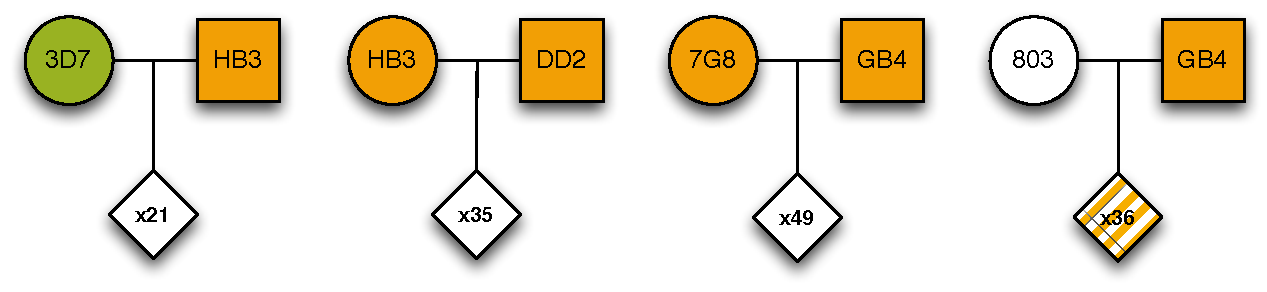
\includegraphics[width=0.9\textwidth]{pfpedigree}
  \caption{Relationships for samples in four \textit{P. falciparum} crosses, with the number of QC-passing Illumina datasets for progeny shown.  Green and orange shading indicates the availability of finished and draft quality reference genomes, respectively.  Orange stripes denote the availability of a draft reference genome for a single progeny, used as validation for \textit{de novo} events.  Gender assignments for the parents are arbitrary, intended only to simplify discussion.}
  \label{fig:pfpedigree}
\end{figure}

\newthought{In the previous chapter, we demonstrated our \textit{de novo} mutation detection} software on simulated crossings of \textit{Plasmodium falciparum} malaria parasites.  We now apply our work to real samples: short-read Illumina data on nearly $150$ isolates taken from four separate crossings of six parasites.

No comprehensive catalog of \textit{de novo} variation in these crosses currently exists.  To date, the focus on the $3D7xHB3$, $HB3xDD2$, $7G8xGB4$ and $803xGB4$ datasets has primarily been on discovering the genomic basis for phenotypic differences between the parents, and on characterizing novel antigenic forms in the children.  However, the previous phenotypic studies have verified the presence of some large structural \textit{de novo} variants - namely a handful of NAHR events involving antigenic genes.  These known events serve as useful validation data for the most difficult form of variation for our software to detect.  Furthermore, these previously observed events have occurred in low-complexity regions.  These regions may confound DNA repair machinery and provide a substrate for the generation of \textit{de novo} variation.  They are typically considered outside the reach of reference-based analyses (which constrain themselves to the roughly $20$ megabases of so-called "core" genome wherein divergence between multiple isolates is much lower and short reads tend to align unambiguously\cite{Miles:2015in}), but may be accessible with our graph-based approach.  Finally, the \textit{P. falciparum} genome is small enough to be sequenced inexpensively on current third generation sequencing platforms, enabling high-quality reconstructions of the parental genomes and even one of the progeny.  The parental samples facilitate DNM discovery, while the child sample serves as a validation dataset with which to evaluate our performance.  These factors make the \textit{P. falciparum} datasets a compelling study target.

\section{Data processing}

\subsection{Initial data}

\begin{table}[]
\centering
\caption{Summary of sequencing data for four \textit{Plasmodium falciparum} crosses}
\label{tbl:crosssummary}
\begin{tabular}{@{}lllll@{}}
\toprule
                & 3D7xHB3       & HB3xDD2       & 7G8xGB4       & 803xGB4             \\ \midrule
Samples         & $22$          & $42$          & $52$          & $36$                \\
Samples QC+     & $21$          & $35$          & $49$          & $36$                \\
Read length     & $76$          & $76$          & $76$          & $100$               \\
Fragment size   & $300 \pm 29$  & $253 \pm 48$  & $293 \pm 21$  & $222 \pm 10$        \\
Coverage        & $99  \pm 38$  & $121 \pm 91$  & $110 \pm 40$  & $205 \pm 106$       \\
Platform        & Illumina GAII & Illumina GAII & Illumina GAII & Illumina HiSeq 2000 \\
Sequencing Date & 2010          & 2009-2012     & 2010-2011     & 2014                \\ \bottomrule
\end{tabular}
\end{table}

We obtained short-read, paired-end whole genome sequence data for parent and progeny clones of the $3D7xHB3$\cite{Walliker:1987cv}, $HB3xDD2$\cite{Wellems:1990eg}, $7G8xGB4$\cite{Hayton:2008hn}, and $803xGB4$ crosses, generously provided to us by the MalariaGen project\footnote{More information, including links to the European Nucleotide Archive where the original reads are stored, can be found at \url{http://www.malariagen.net/apps/pf-crosses/1.0/}.  Note that while the 803xGB4 data we were provided does come to us via MalariaGen, it was provided to them (and subsequently to us) as a personal communication from Michael Krause, Rick Fairhurst \textit{et al.} at the NIAID.  It is not yet part of the public dataset.}.  All samples were sequenced on Illumina platforms over the past five years using a PCR-free library preparation protocol known to reduce coverage biases associated with AT-rich templates.  Avoiding PCR during library construction also removes the issue of replication errors that occur in early cycles being propagated to all subsequent copies, thus masquerading as \textit{de novo} mutations.  Across all four crosses, we obtained $152$ samples prior to any quality control checks.  The data is summarized in Table \ref{tbl:crosssummary}.

\subsection{Data processing for progeny}

\subsubsection{Graph construction}

We built de Bruijn graph structures from the available Illumina data for each child with McCortex's \texttt{build} command, using a kmer size of $47$ bp and discarding bases with a Phred-scaled quality score\cite{Brockman:2008p231} less than $Q5$.  The "dirty" graph (raw graph structure before any pruning is applied) was cleaned using McCortex's \texttt{clean} command, allowing the software to compute cleaning thresholds automatically, and falling back to trimming contiguous regions of the graph with coverage less than $2$ in the event that automatic thresholds could not be calculated.  McCortex's contigs, while strictly speaking not used in our analysis, still serve a useful function in quality control checks.  To generate contigs, paired-end reads were thread through the graph with the McCortex \texttt{thread} command and specifying a minimum fragment size of $0$ bp, maximum fragment size of $400$ bp, and choosing the software's (more conservative) one-way gap-filling procedure.

\subsection{Data processing for parents}

\subsubsection{Graph construction}

\begin{table}[b]
\centering
\caption{Additional data availability for all \textit{P. falciparum} cross parents}
\label{tbl:reflist}
\begin{tabular}{@{}lllllll@{}}
\toprule
                   & 3D7 & HB3 & DD2 & 7G8 & GB4 & 803 \\ \midrule
Finished reference & x   &     &     &     &     &     \\
PacBio assembly    & x   & x   & x   & x   & x   &     \\
Draft assembly     &     & x   & x   & x   &     &     \\
Illumina data      & x   & x   & x   & x   & x   & x   \\ \bottomrule
\end{tabular}
\end{table}

Constructing the parental graphs was a bit more involved than graphs for the children as there were often additional data sources to incorporate.  For five out of the six parents, we benefitted from the availability of supplementary draft assembly data from the Pf3k project.  These draft assemblies were constructed using version $3.0$ of the Hierarchical Genome Assembly Process (HGAP$3$)\cite{Chin:2013iw}.  Briefly, the pipeline performs error correction via the \texttt{Quiver} module, which aligns two-thirds of the data to the longest third, emitting the consensus base and recomputed quality score at each position.  The corrected data is then assembled with a modified version of the Celera assembler\cite{Myers:1995vm}, an overlap-layout-consensus (OLC) assembler originally designed for use on long Sanger reads.  While such reads were typically $500$ bp in length, read lengths from PacBio RS II instruments are on average $10,000$ to $14,000$ bp in length, sometimes as long as $50,000$ bp, two orders of magnitude longer than the reads used to assemble the finished 3D7 reference.  This data helps in determining parental paths in the graph near variants with fewer ambiguities than Illumina data.  Table \ref{tbl:reflist} shows all additional data used in constructing parental assemblies.

Parental graph construction was performed on each parental data source separately following the same workflow used for the children's graphs.  The separate graphs were then combined into a single graph using McCortex's \texttt{join} command.

For most samples, the finished or draft PacBio assemblies vastly outperform any assembly that could be produced with the Illumina data, and are an excellent basis for localizing events and determining their proximity to genes.  However, as there is no high-quality sequence of the $803$ genome, we were forced to construct one ourselves using the available Illumina data.  After producing the cleaned graph with the McCortex workflow, we applied the software's paired-end read threading and contig emission steps.  The assembly statistics for all six genomes are presented in Table \ref{tbl:refstats}.  The assembly for $803$ is exceedingly poor compared to the other assemblies, as expected from short Illumina reads.  That the total sequence length is more than $2.5$ times larger than a typical \textit{falciparum} parasite is artifactual and discussed further below.

\subsubsection{Transfer of gene models}

We transferred gene models onto the new genomes by examining existing finished and draft reference genomes and their annotation sets, selecting each annotated exon sequence from its corresponding FASTA sequence file, and aligning it to the new genome using BWA.  For 7G8, GB4, and 803, we transferred only the 3D7 annotations obtained from PlasmoDB release $26$\cite{Aurrecoechea:2009hh}.  For DD2 and HB3, additional separate annotations exist from the Broad Institute\footnote{\url{http://www.broadinstitute.org/annotation/genome/plasmodium_falciparum_spp/}}.  These undoubtedly contain better representations of genes divergent from their 3D7 counterparts (particularly antigens).  However, owing to the poor DD2 and HB3 assemblies to which they are associated, the annotations are likely to be incomplete.  We therefore chose to transfer both the 3D7 and DD2 (HB3) annotations onto the new DD2 (HB3) assemblies.  This has resulted in a slight over-annotation of genes in these two genomes, as shown in Table \ref{tbl:refstats}.  This happens when the gene models slightly differ between 3D7 and the target (e.g. exon end definitions differ by as much as a single nucleotide), but refer to the same gene.  Rather than simply choosing one definition, we permit both to remain as the PlasmoDB annotations are continuously maintained and improved, while the Broad's annotations have not been updated since April $2014$.

\begin{table}[]
\centering
\caption{Statistics on all parental assemblies}
\label{tbl:refstats}
\begin{tabular}{@{}lllllll@{}}
\toprule
    & contigs & min length & max length & N50       & total sequence & genes            \\ \midrule
3D7 & 16      & 5,967      & 3,291,936  & 1,687,656 & 23,332,831     & 5,777            \\
DD2 & 16      & 6,094      & 3,257,617  & 1,661,885 & 22,682,339     & 8,284 (3D7, DD2) \\
7G8 & 17      & 6,094      & 3,311,228  & 1,560,458 & 22,832,195     & 5,530 (3D7)      \\
GB4 & 26      & 7,376      & 3,360,747  & 1,565,171 & 23,525,386     & 5,576 (3D7)      \\
HB3 & 28      & 6,094      & 3,378,065  & 1,593,993 & 22,812,563     & 7,467 (3D7, HB3) \\
803 & 148,826 & 47         & 17,610     & 1,042     & 59,118,463     & 4,663 (3D7)      \\ \bottomrule
\end{tabular}
\end{table}

\subsubsection{Generation of visualization resources}

We use the Circos\cite{Krzywinski:2009ix} genomic comparison tool to generate whole-genome views of DNM activity in a sample's genome or in all samples from a single cross.  To prepare these visualizations, we require alignments between the contigs of a parental genome and the chromosomes of the reference.  For 3D7, DD2, 7G8, GB4, and HB3, this is trivial as nearly the entirety of each chromosome has been successfully reconstructed.  For those genomes, we simply lined up each assembled contig with its 3D7 counterpart (at the resolution of the image, details of a true alignment cannot be discerned).  In the case of 803, we aligned each contig to the 3D7 genome using BWA to derive the mapping.  

Finally, we computed a number of sequence composition and complexity metrics in tiled $2,500$ bp windows using the SeqComplex tool\footnote{https://github.com/caballero/SeqComplex}.  The full list of metrics computed is as follows:

\begin{enumerate}
\item gc: GC content
\item gcs: GC skew (defined as $(G - C)/(G + C)$)
\item at: AT content
\item ats: AT skew (defined as $(A - T)/(A + T)$)
\item cpg: CpG content
\item ce: Sequence complexity by Shannon entropy\cite{Shannon:1948iy}
\item cl: Sequence complexity by linguistic values\cite{Trifonov:1990vu}
\item cwf: Sequence complexity by Wootton and Federhen\cite{Wootton:1996tu}
\item cz: Sequence compression factor (the ratio of uncompressed to compressed sequence file size, using the \texttt{gzip} compression utility)
\end{enumerate}

These metrics were computed for each parental genome except 803, whose contig lengths were too variable to consistently satisfy the $2,500$ bp window requirement, making comparison with GB4 cumbersome.

\subsection{Quality control}
We examined assembly metrics on all of our samples in order to flag samples for downstream analysis rejection.  We examined each sample for outlier behavior per cross in the number of unique kmers (total number of unique kmers in the graph after the automatic cleaning step - too few kmers indicate poor sequencing quality resulting in most data being thrown away) and contig N50 (the weighted median length of the contigs - very short contigs may indicate high sequencing error rate).  The number of samples retained for analysis is in Table \ref{tbl:crosssummary}.

One expects that a newly assembled \textit{falciparum} parasite should have a similar assembly length to the $3D7$ reference sequence, or at least the other assembled parasites in this dataset.  While this is true for nearly all samples in the 3D7xHB3, HB3xDD2, and 7G8xGB4 crosses, many of the $803xGB4$ samples, shown in Figure \ref{fig:weirdnessAsmLength}, appear to defy this expectation.  Some (including the $803$ parental sample) exhibit assembly lengths well above the $23$ megabases we expect.  Several samples have assemblies in excess of $40$ megabases.  This outcome is unchanged even when other assembly software (e.g. SGA) is applied.  The source of this excess sequence is unclear, but contamination by an organism not present in the BLAST database is a plausible hypothesis.  We note that during investigation of this phenomenon, an update to our BLAST database revealed a number of kmers from the \textit{Pseudomonas} genus that had previously been considered "novel", as the kmers in question were not yet present in the database.  The \textit{Pseudomonas} genus is a family of common environmental bacterium, one of the leading causes of opportunistic human infection\cite{Stover:2000dy}, and around $6.7$ Mbp in length.  It is the subject of drug resistance surveilence\cite{Winsor:2016ca} at many labs including the Wellcome Trust Sanger Institute, where our \textit{falciparum} samples were processed.

For labs that routinely perform a lot of sequencing, it is common for samples from different projects to be prepared simultaneously, and/or for samples to be multiplexed to maximize the use of sequencer capacity, both of which can contribute to sample cross-contamination\cite{Jun:2012je}.  Assembly software does not typically employ contamination checks prior to assembly, instead simply processing any data provided to it.  It is likely that any such contamination would have been assembled and incorporated mostly as disconnected regions of the de Bruijn graph - a series of vertices that do not connect to any other part of the \textit{falciparum} genome.  This might serve to inflate the novel kmer count if the child sample is contaminated but the parents are not, but such regions are easily identified and discarded.  Therefore, we did not treat inflated assembly size to be a QC failure.

\begin{figure}[h!]
  \centering
    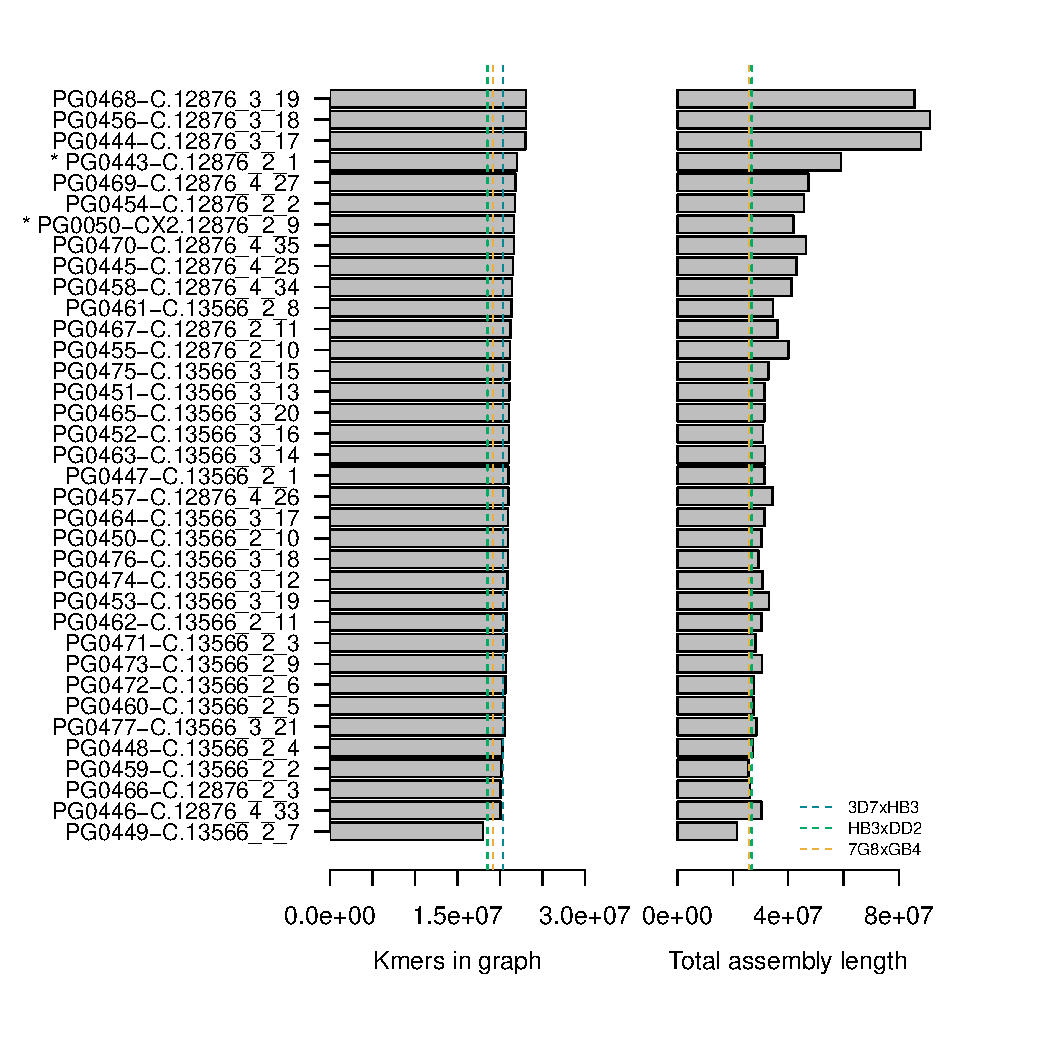
\includegraphics[width=0.5\textwidth]{weirdnessAsmLength-1}
  \caption{Number of kmers and assembly length in the 803xGB4 samples.  Vertical dashed lines indicate the mean value of the metric in other crosses.}
  \label{fig:weirdnessAsmLength}
\end{figure}

\subsection{Data processing for validation isolates}

We selected a number of samples for long-read sequencing on the PacBio RS II instrument.  As of this writing, two samples have been completed: PG0051-C (the 3D7 clone, useful for verifying assembly quality by comparison with the finished 3D7 reference), and PG0446-C (one of the 803xGB4 progeny).  The former was provided by Susana Campino of the Kwiatkowski lab at the Wellcome Trust Sanger Institute.  The latter was provided by Michael Krause and Rick Fairhurst at the Malaria Pathogenesis and Human Immunity Unit at the National Institute of Allergy and Infectious Disease.  Approximately $15~{\mu}g$ of high molecular weight gDNA was provided for each isolate to the CSHL Pacific Biosciences Sequencing Service\footnote{\url{http://cshl.edu/Research/PacBio.html}}.  Sequencing libraries with an average fragment size of $20$ kb were constructed for each sample and size-selected to remove fragments smaller than $7$ kb and larger than $20$ kb using BluePippin.  Optimal loading concentration was determined by choosing a wide range for each of the first $4$ SMRT cells and selecting the concentration that yielded the highest read yield for the remaining SMRT cells.  The PG0051-C isolate was sequenced in late 2014 with the P5-C3 chemistry and assembled with PacBio's HGAP $2.0$ software (assuming a genome size of $23$ megabases).  The PG0446-C isolate, run $16$ months later, was sequenced with the newer P6-C4 chemistry and HGAP $3.0$ software with the same genome size parameter.  Table \ref{tbl:asmstatspacbio} summarizes the sequencing and assembly results on these two isolates.

\begin{table}[]
\centering
\caption{Assembly statistics for PacBio RS II data on PG0051-C and PG0443-C isolates}
\label{tbl:asmstatspacbio}
\begin{tabular}{@{}lll@{}}
\toprule
                        & PG0051-C (3D7)   & PG0443-C (36F11)   \\ \midrule
Chemistry               & P5-C3            & P6-C4              \\
SMRT cells              & $8$              & $9$                \\
Number of reads         & $245,661$        & $282,459$          \\
N50 read length         & $12,968$ bp      & $14,339$ bp        \\
Assembler               & HGAP $2.0$       & HGAP $3.0$         \\
Average contig coverage & $78$x            & $94$x              \\
Polished contigs        & $34$             & $33$               \\ \bottomrule
\end{tabular}
\end{table}

\subsubsection{Establishing assembly quality}
We examined genome recovery and access to massively repetitive sequence (subtelomeric and centromeric regions) that tend to be inaccessible with Illumina sequencing.  PacBio reads were aligned to the finished 3D7 genome using PacBio's \texttt{blasr} long read alignment tool\footnote{\url{https://github.com/PacificBiosciences/blasr}}, while Illumina reads were mapped with the \texttt{bwa mem} tool.  Two such regions in the Illumina and PacBio data for the PG0051-C isolate are shown in Figure \ref{fig:pacbioregions}.  It is evident that the PacBio coverage is roughly uniform across the entire length of the chromosome. In contrast, the Illumina coverage spikes and dips as it moves along, reaching zero coverage in many regions (especially the biologically interesting subtelomeric repetitive regions).

\begin{figure}[h!]
  \centering
    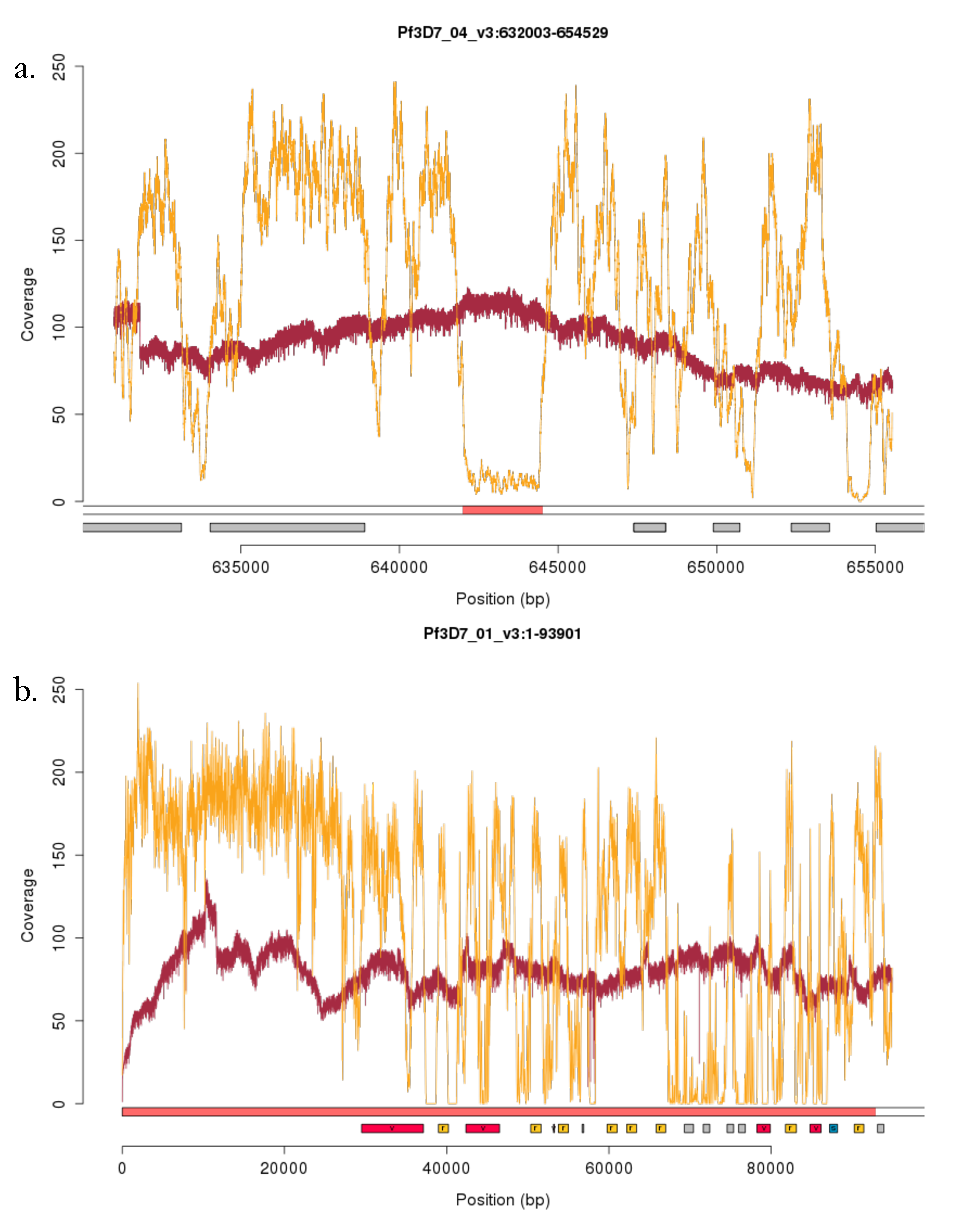
\includegraphics[width=\textwidth]{pacbioregions}
  \caption{Coverage for Illumina data (orange) and PacBio data (red) of the same sample: PG0051-C (the reference isolate, 3D7).  a. Coverage over the chromosome $4$ centromere.  b. Coverage over the $5'$ telomere of chromosome $1$.  Genes from the \textit{var}, \textit{rifin}, and \textit{stevor} antigenic gene families are highlighted and identified with a "v", "r", or "s", respectively.}
  \label{fig:pacbioregions}
\end{figure}

We compared the PacBio-produced assembly of the PG0051-C isolate to the finished reference sequence by performing an all-by-all (contigs versus chromosomes) alignmnt with MUMmer\cite{Versatileandopens:2004dy}.  The alignments are visualized as a multi-dotplot in Figure \ref{fig:dotplot3D7}, an extension of a dot plot that depicts alignments as two dimensional matricies with target and query sequences on the $x$ and $y$ axes, aligning regions of the two sequences shaded accordingly\cite{Gibbs:1970jf}.  Most chromosomes are assembled completely, and the overwhelming majority of the assembly appears on-diagonal (indicating successful one-to-one reconstruction).  Elements appearing off-diagonal could represent misassembly.  However, note that most of these off-diagonal elements occur towards the extremes of each chromosome.  Given that the reference genome was constructed with Sanger reads substantially shorter than the PacBio reads, it is possible some repetitive regions have been collapsed or misplaced, contributing to this nominal error rate.

\begin{figure}[h!]
  \centering
    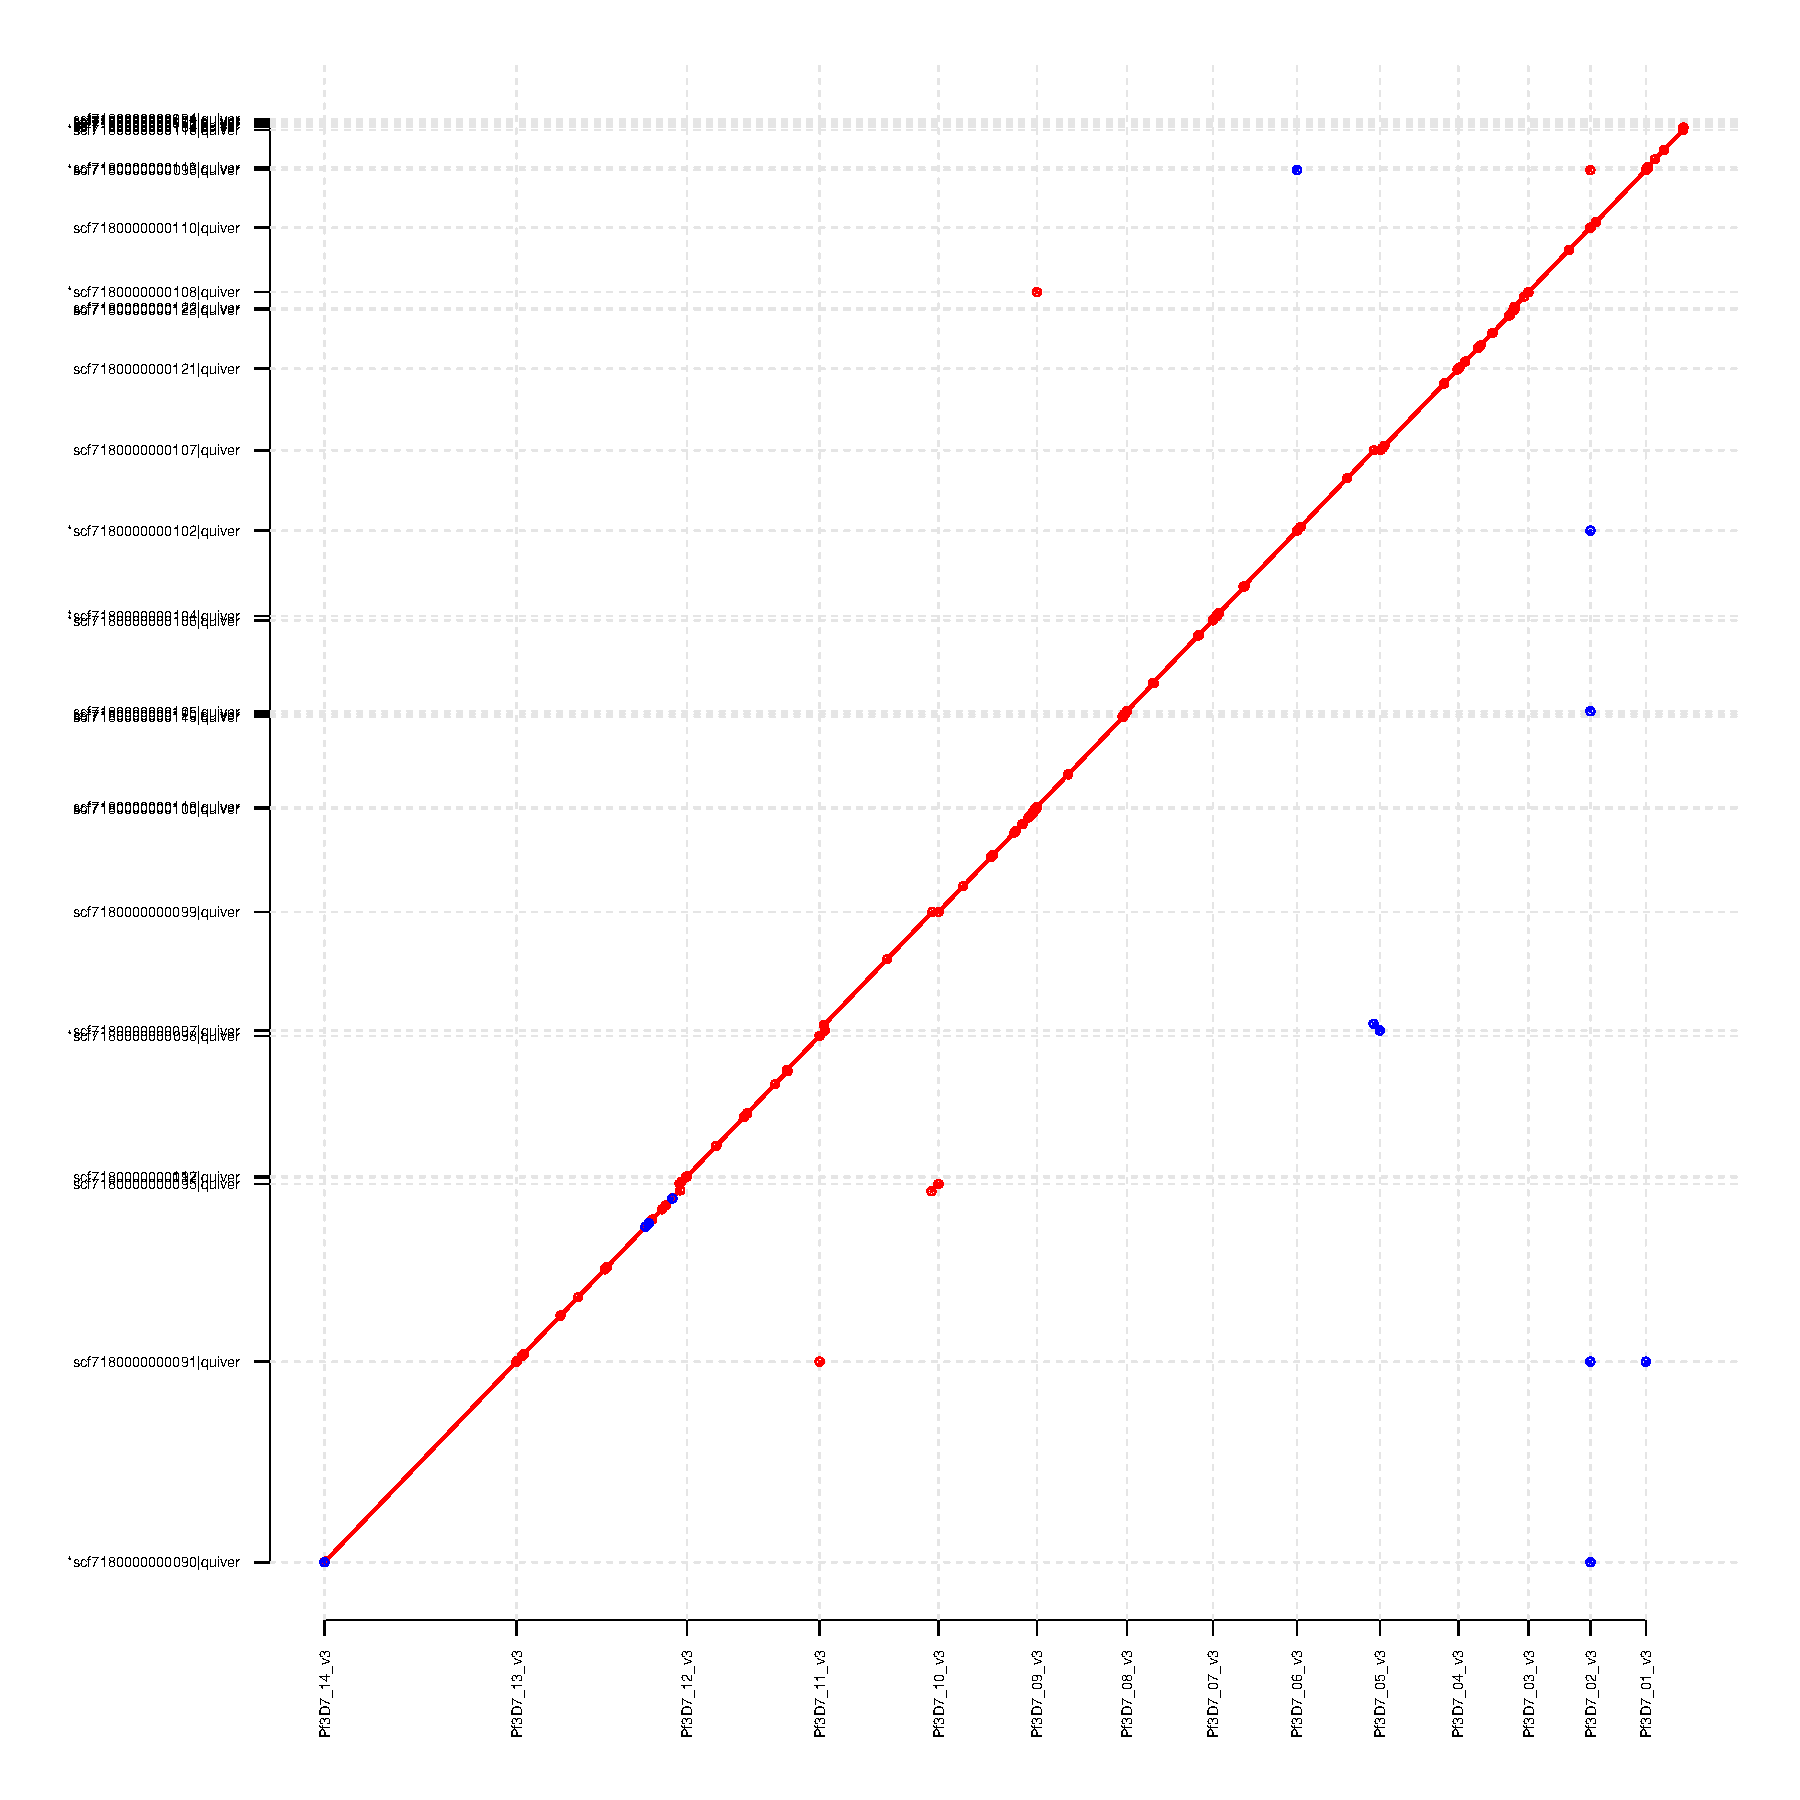
\includegraphics[width=0.7\textwidth]{dotplot}
  \caption{Alignment of contigs from PG0051-C to 3D7 reference assembly}
  \label{fig:dotplot3D7}
\end{figure}

\begin{table}[]
\centering
\caption{Apparent errors per chromosome in the PG0051-C assembly}
\label{tbl:asmerrors}
\begin{tabular}{@{}llll@{}}
\toprule
              & SNP              & INS               & DEL              \\
\midrule
Pf3D7\_01\_v3 & $119~(0.02\%)$   & $763~(0.12\%)$    & $291~(0.05\%)$   \\
Pf3D7\_02\_v3 & $164~(0.02\%)$   & $475~(0.05\%)$    & $162~(0.02\%)$   \\
Pf3D7\_03\_v3 & $272~(0.03\%)$   & $523~(0.05\%)$    & $290~(0.03\%)$   \\
Pf3D7\_04\_v3 & $141~(0.01\%)$   & $856~(0.07\%)$    & $713~(0.06\%)$   \\
Pf3D7\_05\_v3 & $111~(0.01\%)$   & $531~(0.04\%)$    & $175~(0.01\%)$   \\
Pf3D7\_06\_v3 & $504~(0.04\%)$   & $731~(0.05\%)$    & $180~(0.01\%)$   \\
Pf3D7\_07\_v3 & $194~(0.01\%)$   & $609~(0.04\%)$    & $320~(0.02\%)$   \\
Pf3D7\_08\_v3 & $134~(0.01\%)$   & $597~(0.04\%)$    & $251~(0.02\%)$   \\
Pf3D7\_09\_v3 & $61~(0.00\%)$    & $713~(0.05\%)$    & $259~(0.02\%)$   \\
Pf3D7\_10\_v3 & $732~(0.04\%)$   & $810~(0.05\%)$    & $308~(0.02\%)$   \\
Pf3D7\_11\_v3 & $310~(0.02\%)$   & $1,008~(0.05\%)$  & $459~(0.02\%)$   \\
Pf3D7\_12\_v3 & $232~(0.01\%)$   & $1,202~(0.05\%)$  & $390~(0.02\%)$   \\
Pf3D7\_13\_v3 & $231~(0.01\%)$   & $1,493~(0.05\%)$  & $409~(0.01\%)$   \\
Pf3D7\_14\_v3 & $152~(0.00\%)$   & $1,309~(0.04\%)$  & $396~(0.01\%)$   \\
Total         & $3,357~(0.03\%)$ & $11,620~(0.10\%)$ & $4,603~(0.04\%)$ \\
\bottomrule
\end{tabular}
\end{table}

As we have sequenced DNA from the 3D7 parasite, any differences should likely reflect errors in the sequence. We therefore called SNPs between the two assemblies to find these errors. The sums are presented in Table \ref{tbl:asmerrors}, as well as the percent of bases per chromosome these errors represent.  Overall, the SNP, insertion, and deletion rates are exceedingly low: amounting to 19,580 events in a 23 megabase genome (0.17\%). The insertion rate is much higher than that of deletions and SNPs, perhaps due to the dominant insertion error mode of the PacBio sequencing instrument. All chromosomes appear reasonably similar in performance.

We examined the recovery of the $62$ members of the \textit{var} gene family by aligning their full-length genomic sequences (exons and introns) to the PG0051-C assembly using \texttt{bwa mem}. All $62$ \textit{var} genes were successfully aligned to the assembly (all had mapping quality greater than $0$; only $1$ had mapping quality less than 60).  $21$ were found to map with $100\%$ identity. The remaining have, on average, $2.46$ mismatches, $1.39$ insertions, and $0.63$ deletions. The overwhelming majority of indels are a single nucleotide in length.

It seemed likely that many of these errors occur in intronic regions where high repetitive sequence content might contribute to misassembly. We investigated this hypothesis by aligning the exons of the \textit{var} genes separately and enumerating errors observed in exons and introns. We ignored $11$ genes with poor exon alignments (i.e. with mapping quality less than $10$). $91.78\%$ of the errors are found in intronic regions. In all cases, exon $2$ of the \textit{var} gene (the short exon) is base-for-base perfect when compared to the canonical reference.

Based on these measurements of the error rate, we estimate the quality of the PacBio assembly of the PG0051-C (3D7) isolate to be approximately $Q31$\footnote{$Q = -10{\log}_{10}(q) = -10{\log}_{10}((11,620 + 4,603 + 3,357)/23,332,831)$}, or less than one error per thousand bases.  We note that this is a pessimistic estimate, based on the assumption that any differences between this and the reference assembly indicate errors in our assembly.  In long, repetitive regions of the genome, this assumption may not be accurate.

\subsubsection{Preparing the validation isolate reference}

\begin{figure}[h!]
  \centering
    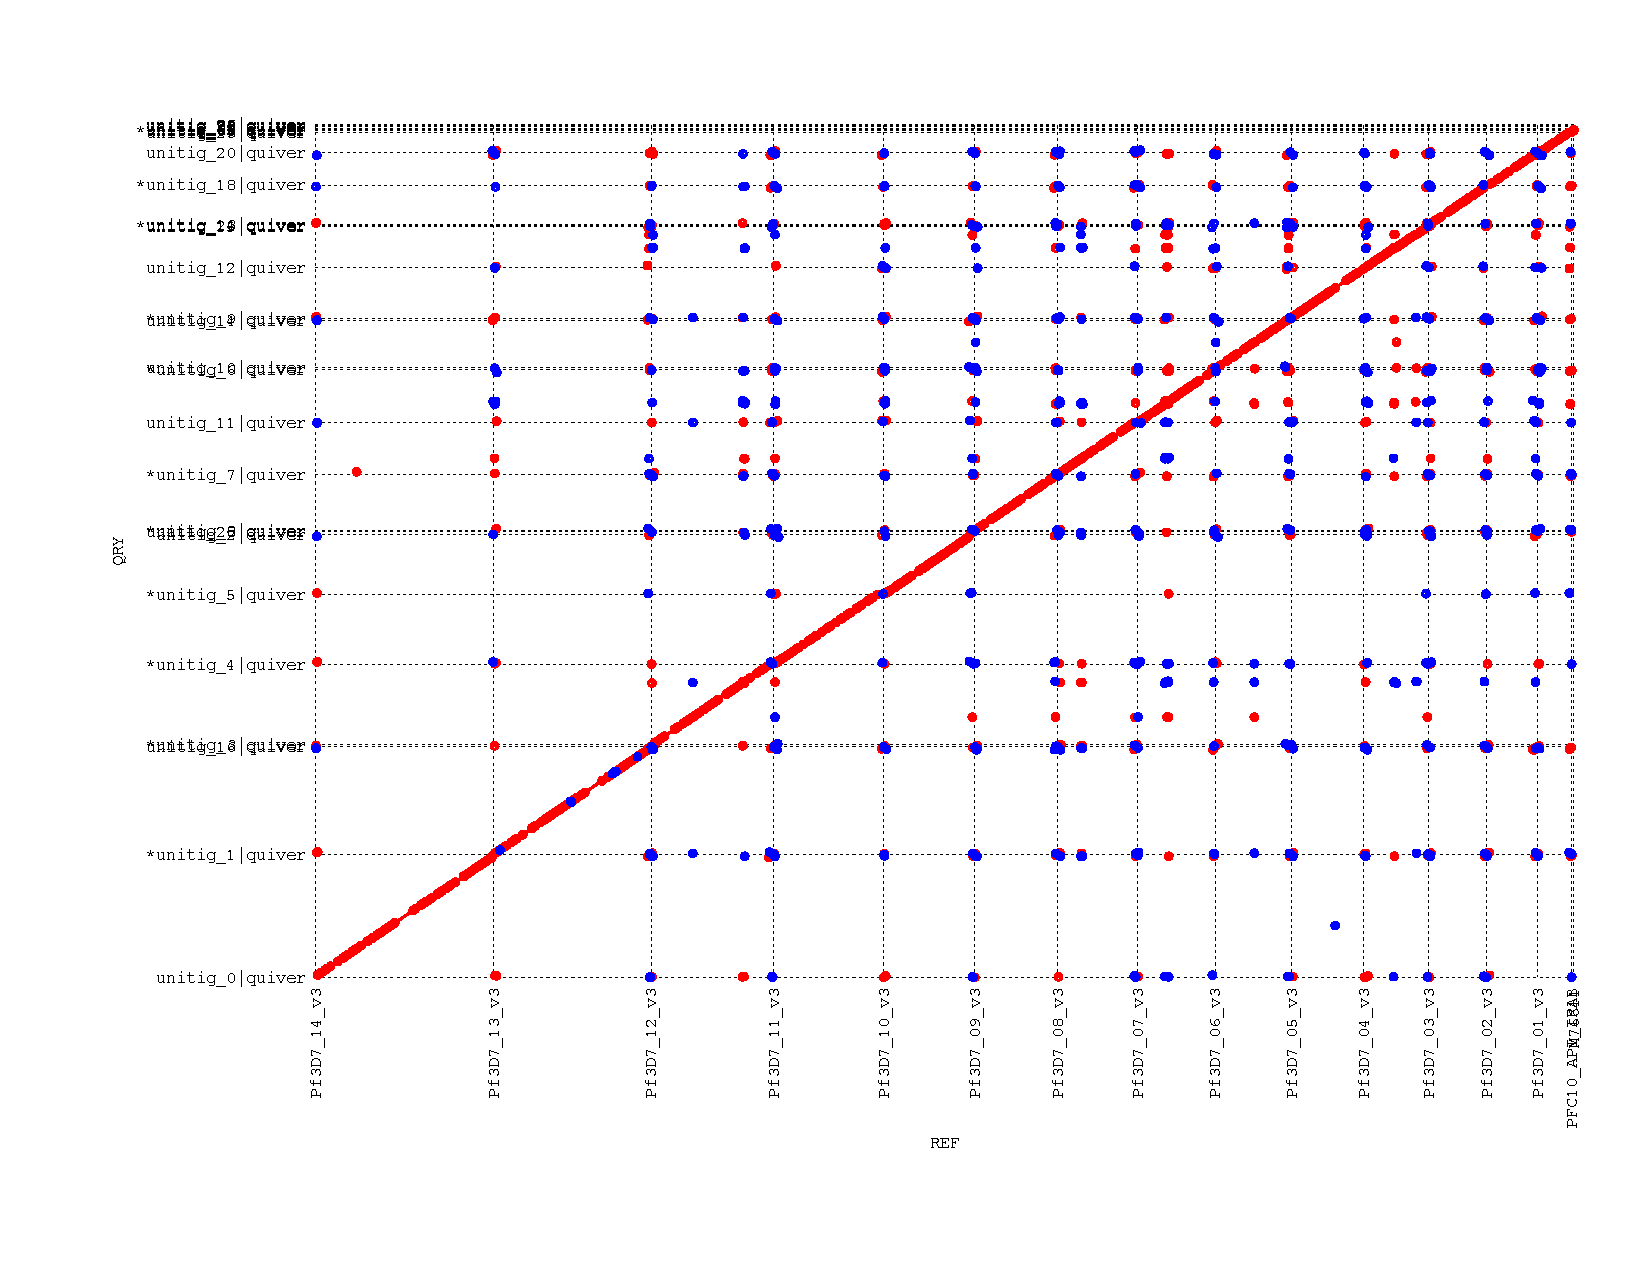
\includegraphics[width=\textwidth]{36F11dotplot}
  \caption{Alignment of contigs from PG0443-C to 3D7 reference assembly}
  \label{fig:valdotplot}
\end{figure}

Having established the performance of the instrument and assembler in providing a viable assembly for a \textit{P. falciparum} isolate, we turned our attention to the validation sample from the 803xGB4 cross, PG0446-C.  We aligned the isolate's assembly to the 3D7 reference sequence using MUMmer, shown in Figure \ref{fig:valdotplot}.  Note that compared to the PG0051-C isolate, the validation isolate has much more off-diagonal activity, particularly towards the telomeres.  This is to be expected.  While the core genome between isolates is expected to be relatively stable, tremendous immune pressure has forced the antigenic repertoire to diversify rapidly.  These genes, primarily located in the subtelomeric regions, are the regions that land off-diagonal, indicative of the extensive recombination and mutation history.

We relabelled and reoriented each contig as necessary based on the alignment so as to more easily establish genomic positioning of events during analysis.  The assignments and orientation were further validated by transferring 3D7 gene model annotations onto the PG0446-C assembly by aligning each exon with \texttt{bwa mem}, operating under the assumption that the core genome is reasonably stable between isolates and that properly labelled and oriented contigs will yield exon alignments that match orientation and approximate positioning between the two assemblies.  Figure \ref{fig:loadGff} shows an example for chromosome $1$.  The vertical offset of all points is due to the fact that the assembly length of chromosome $1$ in the PG0446-C assembly is longer than the reference length.  Only exons towards the telomeric ends of the chromosome are misplaced, evidently originating from chromosomes other than chromosome $1$.  All other chromosome $1$ exons are aligned with the expected position and orientation.

After chromosome identification, we observed a handful of contigs that could not be assigned a place in the nuclear genome.  After running each unplaced contig through BLAST, we discovered two long contigs (thousands of bp) and nearly perfect hits to various species in the \textit{Pseudomonas} genus.  Discovering this contamination in the PacBio assembly and the Illumina samples strongly suggests the samples are contaminated at the source, contributing to the inflated 803xGB4 assembly lengths.  We removed these contigs from our assembly.

\begin{figure}[h!]
  \centering
    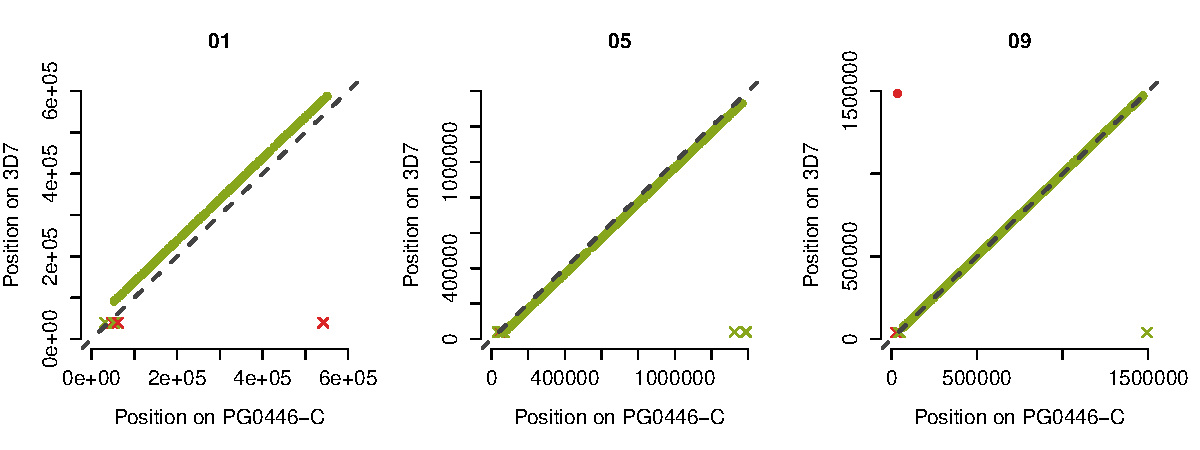
\includegraphics[width=\textwidth]{twochrs-1}
  \caption{Placement and orientation of exons from the reference assembly mapped to the PG0446-C assembly.  Chromosomes $1$, $5$, and $9$ shown.}
  \label{fig:loadGff}
\end{figure}

We verified sample identity by slicing the PacBio assembly into $1,000$ bp tiles (non-overlapping), aligning each tile to the 3D7 reference genome using \texttt{bwa mem}, and genotyping sites found to be variant in the MalariaGen 803xGB4 callset using the Genome Analysis Toolkit module, \texttt{UnifiedGenotyper} (specifying the genotype likelihood model to "SNP", ploidy to $1$, genotyping mode to "GENOTYPE\_GIVEN\_ALLELES", assuming default base quality scores should be $Q30$, and providing the 803xGB4 alleles from MalariaGen)\footnote{This procedure, while admittedly a bit indirect, provides vastly better results than genotyping the PacBio reads directly.  The assembly contains far fewer errors than the reads, even after error correction.  It is also much more straightforward than processing the MUMmer variant output, which uses a different file format to VCF, making comparisons cumbersome.}.  Chromosome $14$ is shown in Figure \ref{fig:showHaps}.  Note that while the PacBio sample's crossover pattern does appear to match that of PG0446-C, samples PG0445-C, PG0453-C, and PG0457-C also share the same pattern.  This common pattern is observed for these samples on all chromosomes.  These samples are almost certainly clones of one another.

\begin{figure}[h!]
  \centering
    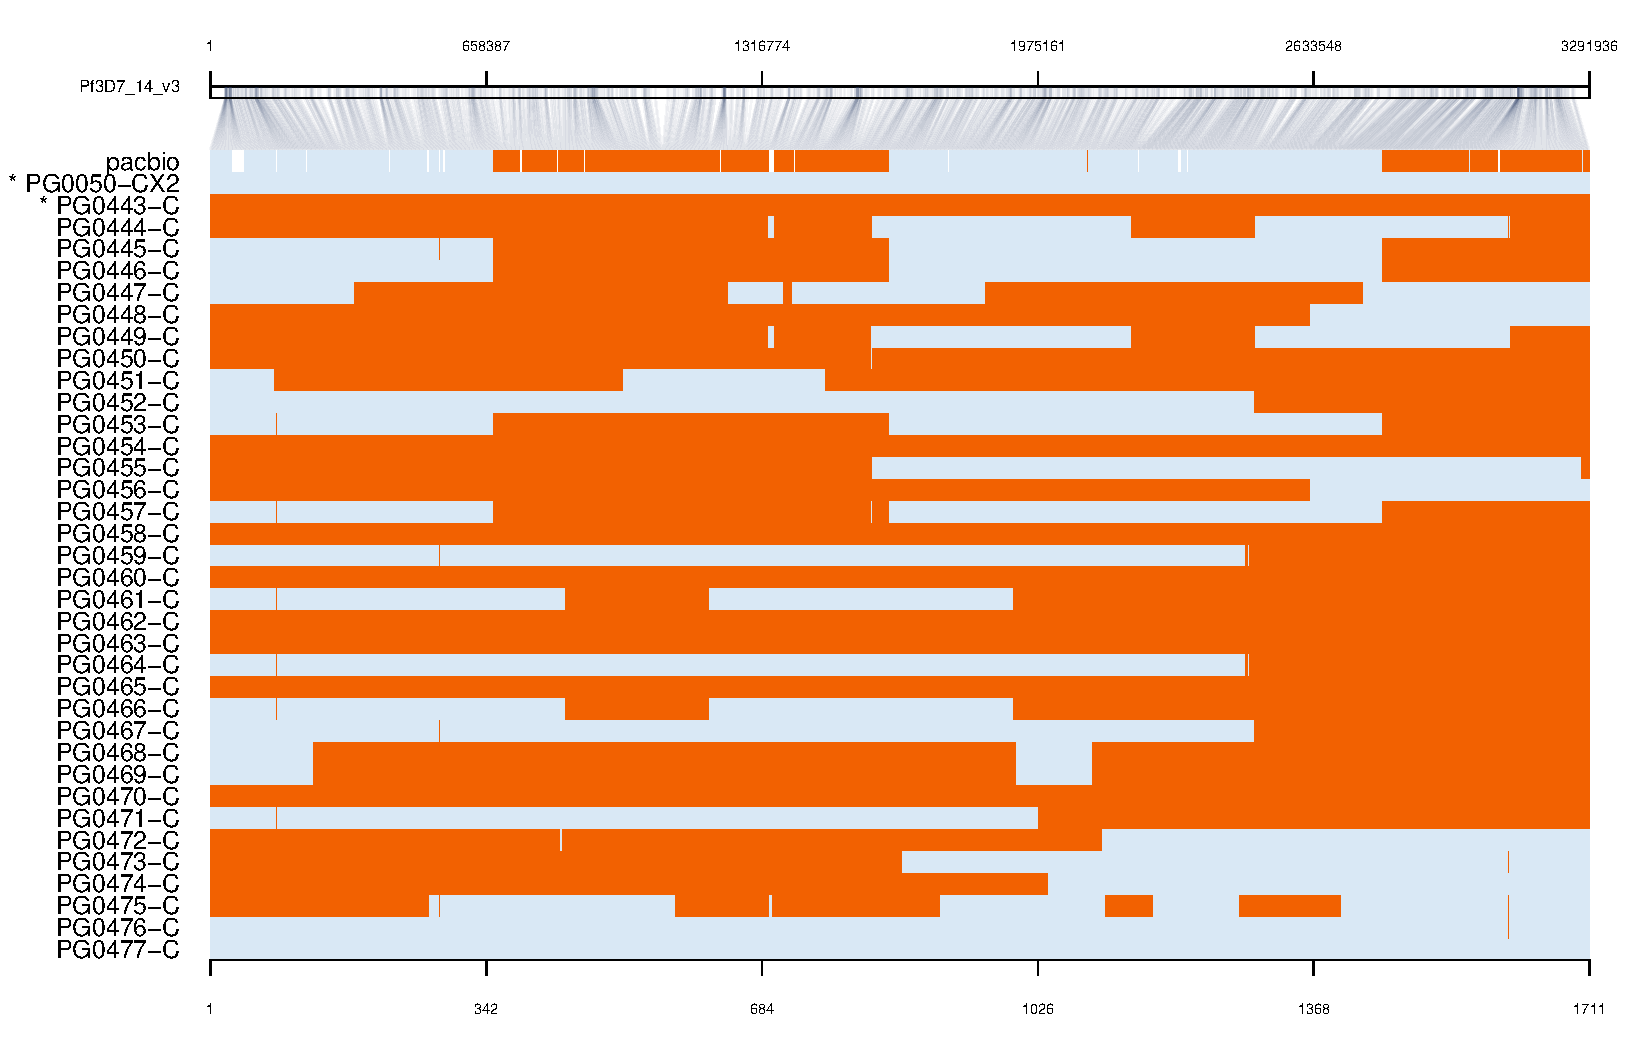
\includegraphics[width=\textwidth]{showHaps-14}
  \caption{Haplotype mosaic for chromosome $14$ in the 803xGB4 cross dataset.  Parental samples are identified with asterisks.  For remaining samples, alleles are color-coded according to the parent from which they are apparently inherited - orange for mother (PG0443-C, the 803 isolate), blue for father (PG0050-CX2, the GB4 isolate).  Missing data (sites where no genotype could be ascertained) are shown in white.  Bottom axis represents variant number.  Top axis represents variant position along the length of the chromosome.}
  \label{fig:showHaps}
\end{figure}

\section{Comparison to validation isolate}

\subsection{Verification of novel kmers}

As we have demonstrated that the PacBio assembly of the validation isolate is high-quality, novelty found in the Illumina dataset for the same sample can be verified by examining the PacBio isolate.  At the filtration levels of "all", "confident", and "trusted", initial processing of the Illumina data for 803xGB4 sample PG0446-C was found to have $28,904$; $17,069$; and $8,197$ novel kmers, respectively.  The PacBio assembly of the same sample recapitulates only $1,639$; $802$; and $48$ novel kmers, respectively.  The discrepancies can be largely attributed to three (not necessarily independent) factors: an over-aggressive lower threshold for coverage, no upper threshold, and significant data contamination.

The first two points regarding coverage can be observed in Figure \ref{fig:covdists}a-c.  The leftmost panel shows a clear valley between the left end of the distribution (presumably sequencing errors, as they are so rarely observed in the dataset) and the first local maximum (likely real data).  In the middle panel, kmer coverage in PG0446-C decays more smoothly, and it is far less obvious as to where the lower threshold should be placed\footnote{It is worth mentioning that the PG0446-C sample, sequenced on more modern Illumina HiSeq 2000 platforms, likely enjoys a much lower sequencing error rate than the Illumina GAII used for PG0055-C, which contributes to our difficulty in automatically finding a reasonable coverage threshold.}.  In the rightmost panel, all novel kmers are shown, conditional to being present or absent in the PacBio assembly of the same sample.  Our automatically calulated threshold is clearly set too high, as it is slicing through the middle of the coverage distribution for novel kmers recapitulated by the PacBio dataset.

Furthermore, the rightmost panel shows a number of coverage outliers in the set of novel kmers that are not present in the PacBio dataset.  While their source is not immediately apparent, it is clear they have a large contribution to the set of novel kmers we examine; $1,057$ kmers present in the Illumina dataset but absent in the PacBio dataset were found to be high coverage outliers.

\begin{figure}[h!]
  \centering
    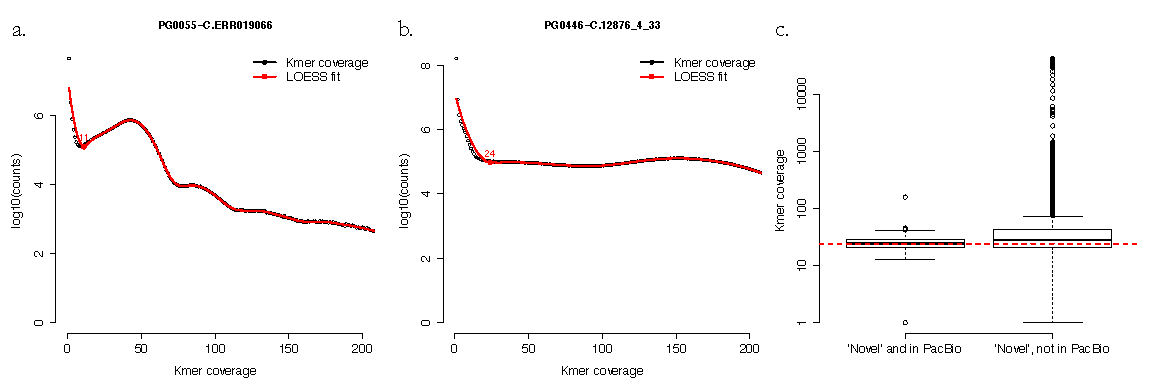
\includegraphics[width=\textwidth]{covdists}
  \caption{a. Kmer coverage in a 3D7xHB3 sample, with calculated lower threshold shown in red.  b. Kmer coverage in the 803xGB4 sample, PG0446-C, with calculated lower threshold shown in red.  c. Kmer coverage distributions for all novel kmers in PG0446-C, conditional on the kmer being present or absent in the PacBio assembly.  Calculated lower threshold from panel b shown in red.}
  \label{fig:covdists}
\end{figure}

We investigated other potentially erroneous novel kmers: putative novel kmers absent from the PacBio assembly and with coverage between $10x$ and $74x$.  We discovered many of these novel kmers exist in branches that either never connect with the graphs of the parents (we refer to these as "orphan" branches, Figure \ref{fig:orphans}a), or connect suspiciously amidst a number of putatively novel kmers rejected by the contamination checks (we refer to these as "bushy-tailed" branches, Figure \ref{fig:orphans}b).  Both appear to be symptoms of unrecognized contamination, owing to the fact that the BLAST database is not (and can never be) complete.  In attempting to remove any contribution to the graphs from non-target sources, it is insufficient to discard only the kmers that appear in the BLAST database.  Sequencing centers will always be sequencing new organisms, and the contents of the BLAST database will necessarily lag behind.  Discarding orphan branches is straightforward, but incompletely treats the problem; the bushy-tailed branches erroneously connect with the parental graphs and must be removed as well.

Finally, we discovered a substantial source of erroneous novel kmers stemming from "overcleaning", an issue wherein some kmers representing true genomic sequence are mistaken for sequencing error and removed from the graph via the assembler's error-cleaning or error-correcting process.  When this occurs in the parents but not the child (often due to coverage fluctuations), a kmer can appear to be "novel".  To mitigate this issue, we inspect the child's cleaned graph and the parents' dirty graphs.  However, a region of low coverage can also be flanked by regions of \textit{no} coverage; there are many kmers that are likely present in the parental genomes, but unobserved by chance.

\begin{figure}[h!]
  \centering
    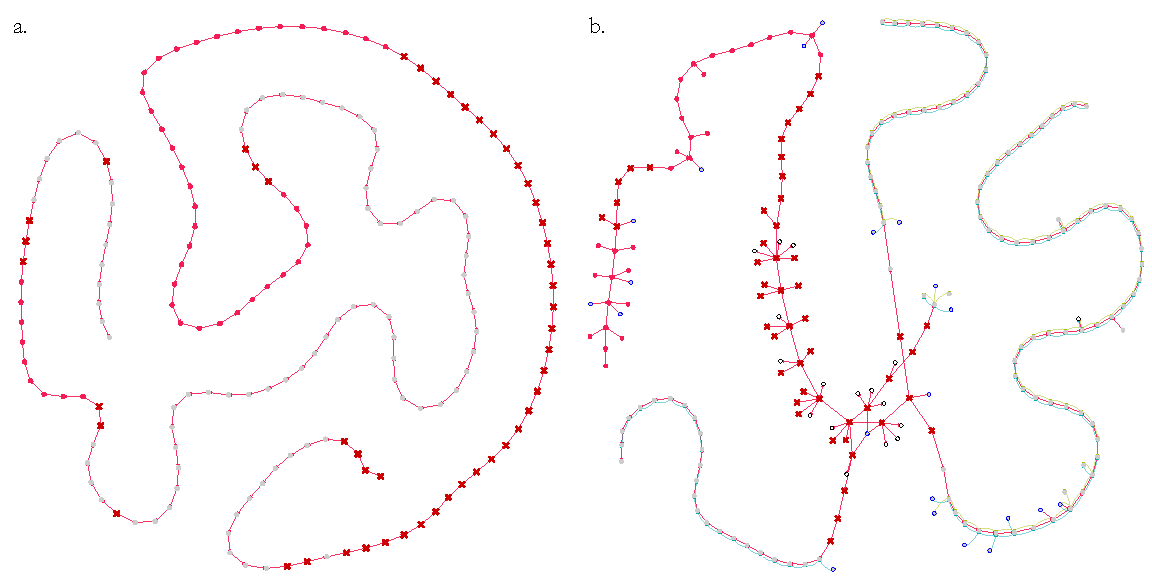
\includegraphics[width=\textwidth]{orphans}
  \caption{Local subgraphs in the Illumina data for PG0446-C near novel kmers that are absent in the corresponding PacBio assembly.  Red circles denote "trusted" novel kmers (those that passed our initial coverage and contamination checks).  Red crosses indicate "untrusted" novel kmers (those that passed our initial coverage check but failed the contamination check).  a. An "orphan" branch: a series of novel kmers not connected to the parental graphs.  b. A "bushy-tailed" branch: a series of novel kmers that appear to connect to everything, including the parental graphs, by chance.}
  \label{fig:orphans}
\end{figure}

To resolve these issues, we implemented a filtering solution for novel kmers in four parts.  First, we implemented a manual procedure for specifying coverage limits, selecting a lower limit of $10x$ and an upper limit of $74x$.  Next, we implemented software to explore the trio graph starting at confident novel kmers rejected by the contamination filter using our condition-limited depth first search software.  Explored branches containing novel kmers that are on the same branch as rejected kmers are similarly tagged for rejection.  Third, we explore the trio graph starting with remaining confident novel kmers.  If the explored subgraph does not connect with the parental graphs in any way, the kmers in the branch are marked for rejection and removed from further consideration.  Finally, we examine contigs with "overcleaned" novel kmers (i.e. any kmer that would be considered novel by comparing to the cleaned parental graphs, but is subsequently denied this label after examining the dirty parental graphs).  Novel kmers found on the same contig are considered tainted and removed from consideration.  Any putatively novel kmer surviving this battery of tests is considered "filtered".

The results of our novel kmer filtering are shown in Figure \ref{fig:novelfilter}.  $95$ kmers survive our battery of filters to be considered truly novel sequence in the genome of the PG0446-C child.  We called DNMs in the Illumina data using our graph-based calling software and discovered three events: two SNPs ($47$ kmers each) and a single kmer occurring in a repetitive region of a telomere; the precise nature of this single-kmer event is not clear.  The PacBio dataset contains $51$ novel kmers, $48$ of which overlap our calls (one SNP and the unknown event).  The other $47$ kmers from the second SNP are not present in the PacBio assembly.  However, manual inspection reveals this SNP to be polymorphic, possibly indicating a \textit{de novo} mutation that has occurred in the sample during mitosis that has not yet reached fixation in the sequenced population of cells.  It is likely that the event (shown in Figure \ref{fig:fpcomp}) is a true variant, absent in the PacBio assembly as the Celera assembler is forced to make a choice between which allele to retain in the haploid assembly.  The presence of the alternate allele in the uncorrected PacBio reads strongly suggests this is event is real and its absence from the assembly is an artifact of the assembler's bubble-popping procedure.  The remaining $3$ kmers from the PacBio dataset are not called in the Illumina data as they are low coverage (all at $1x$ coverage, all low complexity sequence, possibly representing recurrent sequencing errors in both the PacBio and Illumina data).

\begin{figure}[h!]
  \centering
    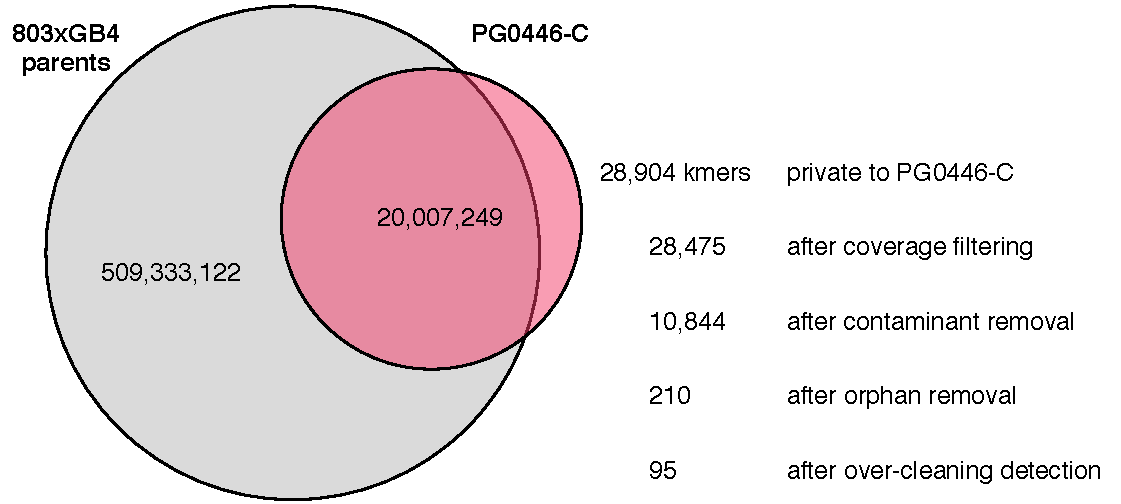
\includegraphics[width=\textwidth]{novelfilter}
  \caption{The results of filtering kmers private to the PG0446-C child }
  \label{fig:novelfilter}
\end{figure}

Based on the kmer recovery results listed above, our sensitivity to novel kmers is between $94\%$ and $100\%$ (depending on whether the $3$ missed kmers are considered truly novel kmers or sequencing errors), and specificity is greater than $99\%$.  Both SNPs and the unknown third event are recovered successfully.  The two SNPs are shown in Figures \ref{fig:pacbiohomsnpigv} (A to G, $13:2,032,381$) and \ref{fig:pacbiohetsnpigv} (C to T, $14:1,396,035$, a non-synonymous substitution resulting in a T to I amino acid change).  Figure \ref{fig:pacbiounknownigv} shows the third, unknown event.

\begin{sidewaysfigure}[h!]
  \centering
    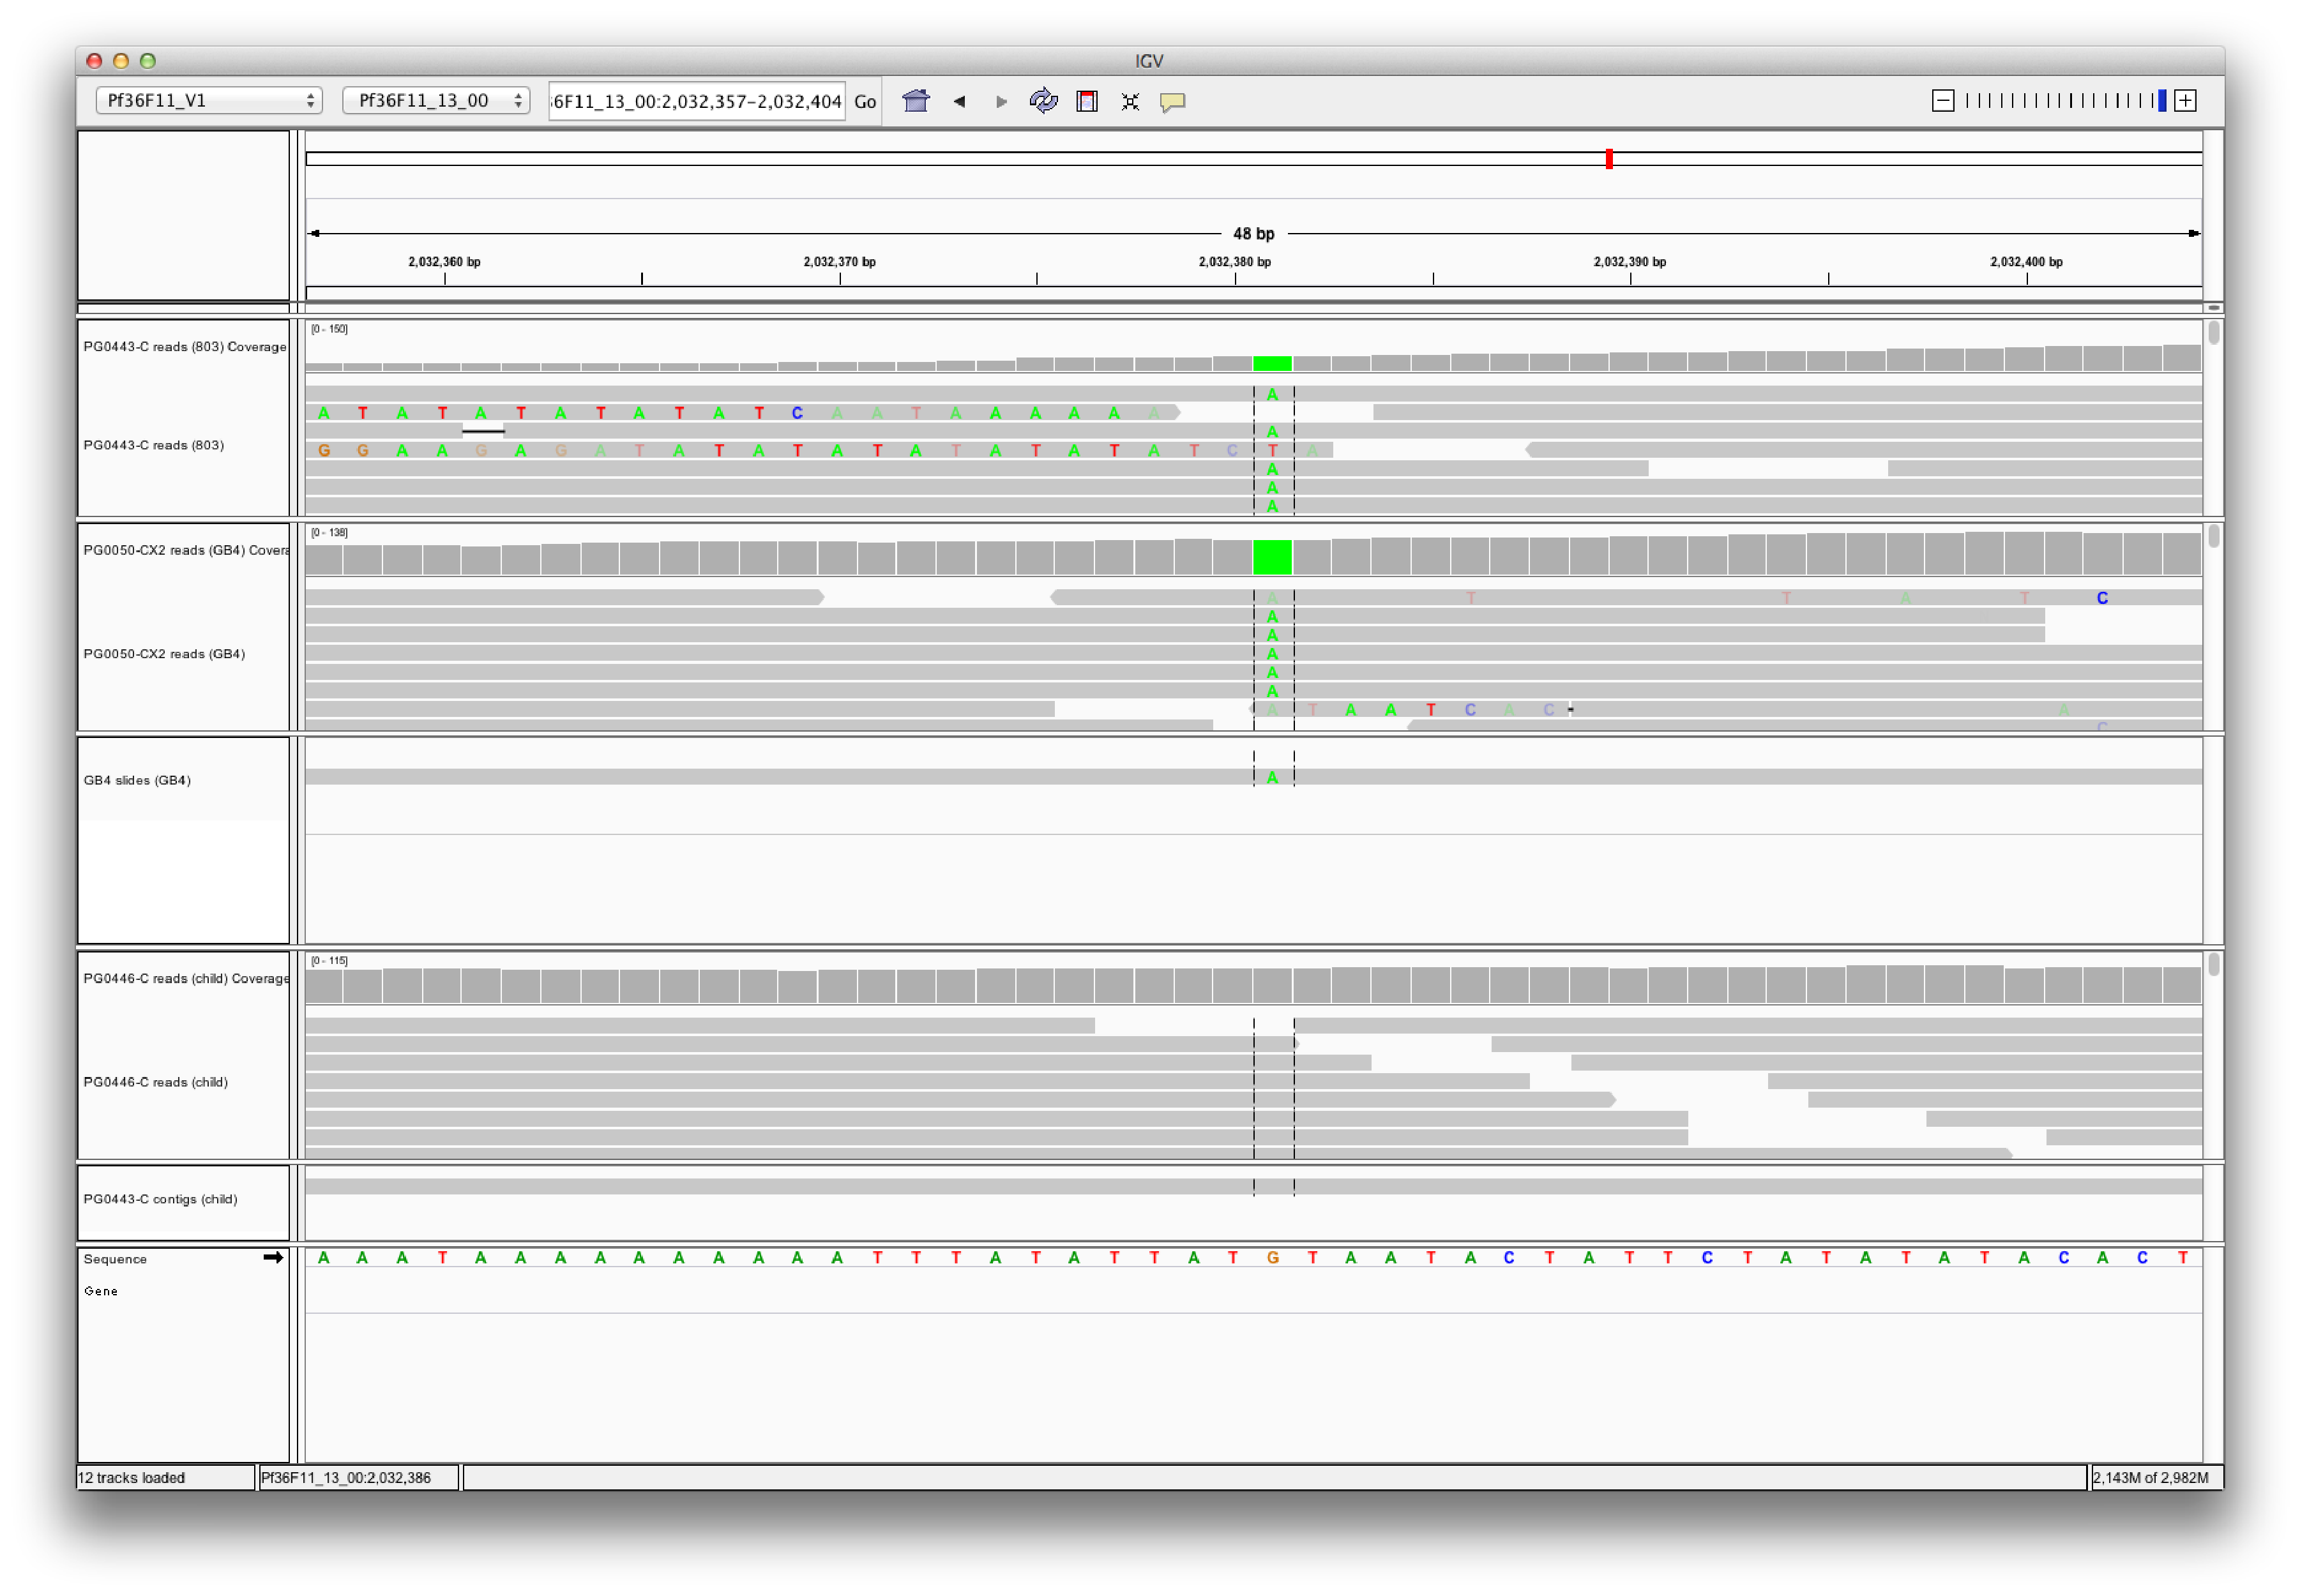
\includegraphics[width=\textwidth]{pacbiohomsnpigv}
  \caption{IGV screenshot of an A to G SNP, showing reads and assembly information for the trio, aligned to the PacBio PG0446-C assembly.  Top panel: 803.  Middle two: GB4 reads and PacBio assembly (sliced to facilitate alignment).  Lower two: PG0446-C reads and contig containing the variant in question from the a. panel.}
  \label{fig:pacbiohomsnpigv}
\end{sidewaysfigure}

\begin{sidewaysfigure}[h!]
  \centering
    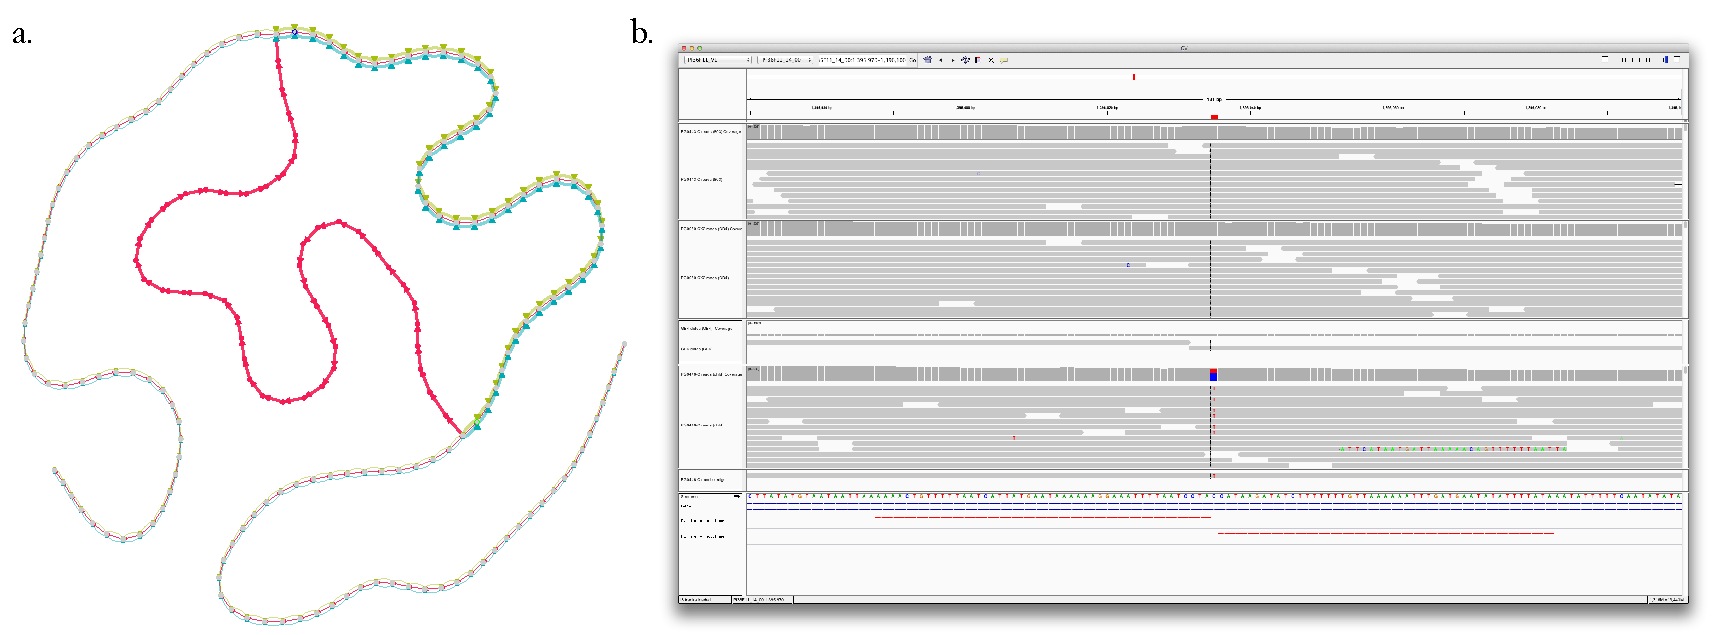
\includegraphics[width=\textwidth]{fpcomp}
  \caption{A C to T SNP that has likely not reached fixation in the sequenced population of ostensibly clonal parasites.  a. Local subgraph at the site, wherein the child's graph contains paths that traverse the series of novel kmers as well as the parental kmers, indicating polymorphic status.  b. IGV screenshot of the site showing reads and assembly information for the trio, aligned to the 3D7 reference genome.  Top panel: positions of the called variants in the reference-basde analysis.  Second panel: PG0443-C (803).  Third: PG0050-CX2 (GB4).  Fourth: PG0446-C (child).  Fifth: Uncorrected PacBio reads from PG0446-C.  Bottom: gene model track from PlasmoDB $9.0$.  Stacked barplots above tracks indicate the proportion of reads supporting each allele.}
  \label{fig:pacbiohetsnpigv}
\end{sidewaysfigure}

\begin{sidewaysfigure}[h!]
  \centering
    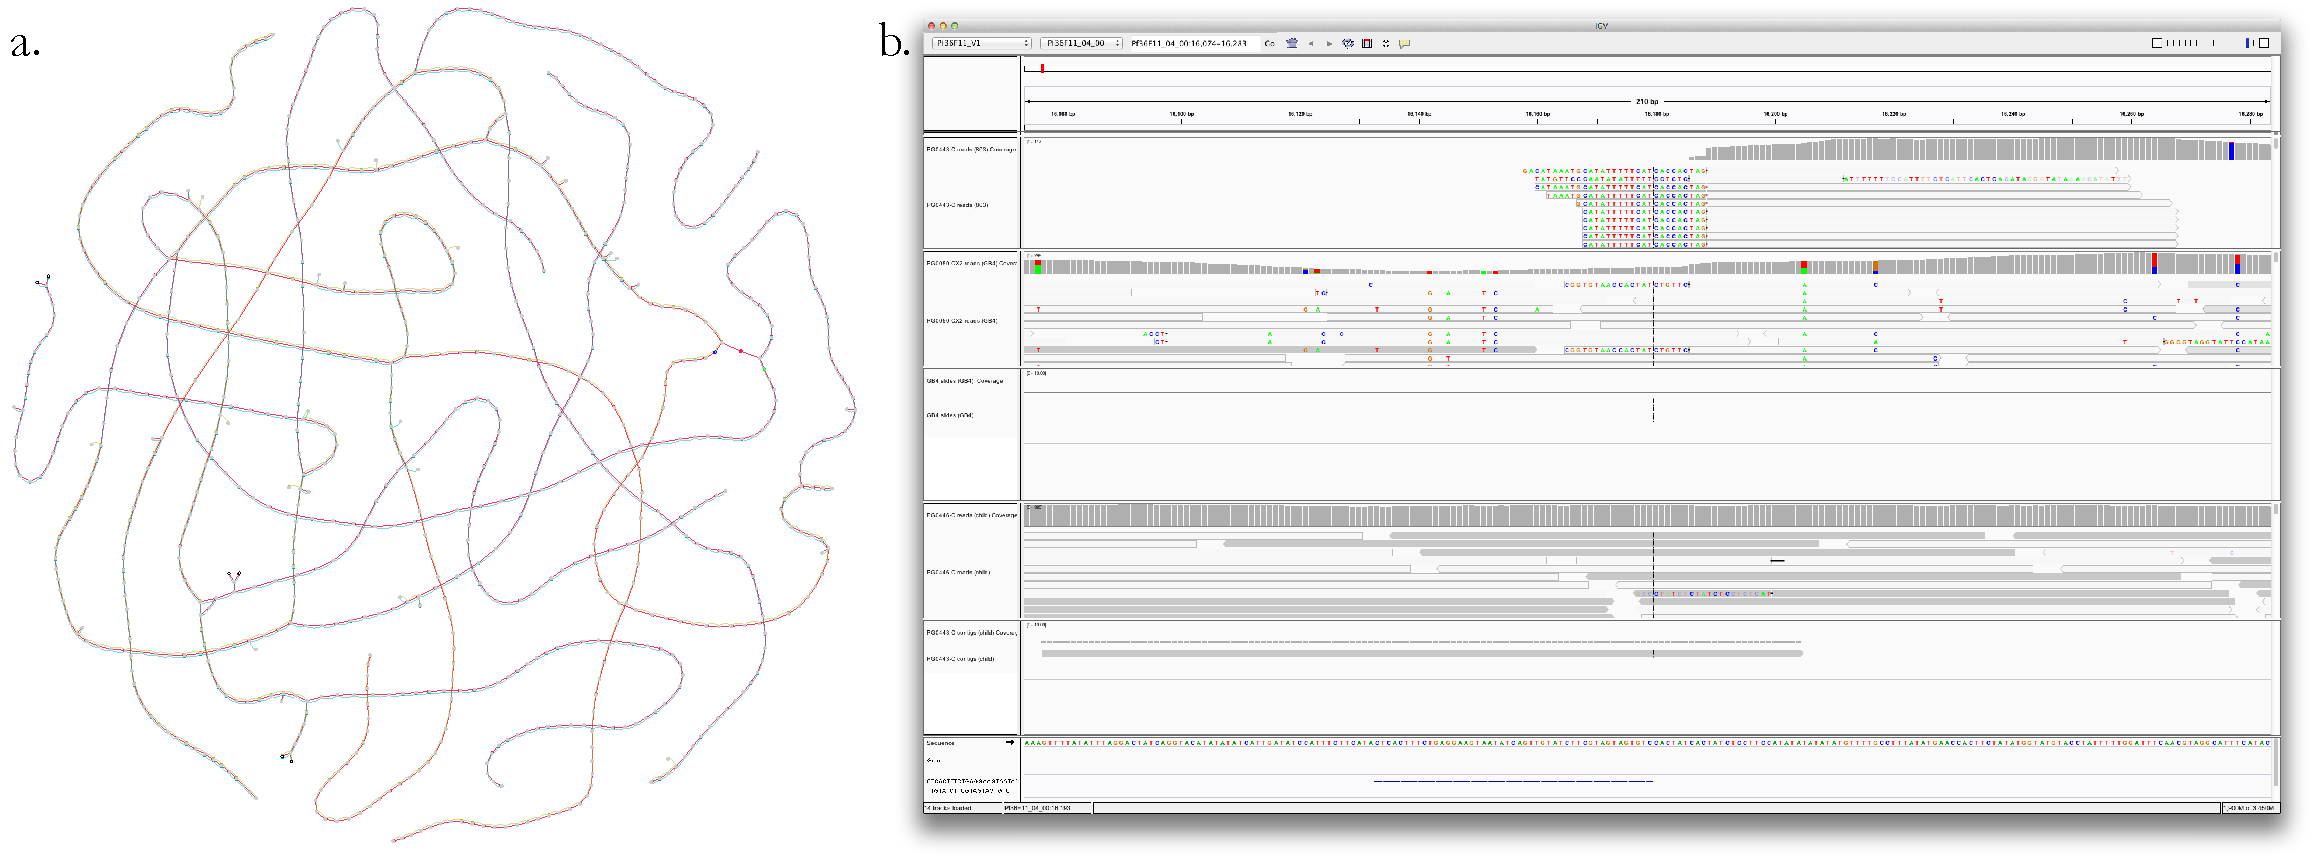
\includegraphics[width=\textwidth]{weirdsinglenovelkmercomp}
  \caption{A strange event involving a single novel kmer.  a. Local subgraph at the site; the novel kmer in question is depicted as a filled red vertex in the right side of the image.  b. IGV screenshot of the site showing reads and assembly information for the trio, aligned to the PacBio PG0446-C assembly.}
  \label{fig:weirdsinglenovelkmercomp}
\end{sidewaysfigure}

\subsection{Comparison to reference-based analysis}

We sought to determine our relative ability to detect DNMs accurately compared to that of the reference-based analysis.  As the release version of the MalariaGen callset purposefully excluded \textit{de novo} mutations (attempting to minimize Mendelian error rates to ensure high confidence in the inherited variation callset), we set about we processing the Illumina data from the PG0446-C trio (PG0443-C (803), PG0050-CX2 (GB4), and PG0446-C) ourselves.  Reads were aligned with \texttt{bwa mem} to the 3D7 reference genome, release $9.0$ from PlasmoDB.  PCR duplicates were marked with the \texttt{MarkDuplicates} program from the Picard suite; these marked reads were subsequently ignored in downstream processing.  A list of genomic regions with reads appearing to span indels were discovered using the GATK's \texttt{RealignerTargetCreator} module (supplemented by MalariaGen's 803xGB4 calls as additional candidate regions to consider).  We subsequently ran the GATK's \texttt{IndelRealigner} to perform the local realignments on these candidate regions.  We recalibrated base quality scores using the GATK's \texttt{BaseRecalibrator} tool, once again supplying the MalariaGen calls as sites to ignore when computing the data error model.  Variants were called across the PG0443-C, PG0050-CX2, and PG0446-C samples simultaneously using the GATK's \texttt{HaplotypeCaller} module, which performs local \textit{de novo} assembly to determine the haplotype sequence at so-called "active sites", windows of the genome detected to harbor some sort of variation.  For each approach, we specified a ploidy of $1$.  SNPs and indels were filtered separately using the GATK's \texttt{VariantRecalibrator} tool, supplying the MalariaGen calls as training data.  We set the desired truth sensitivity to $99\%$ (i.e. requesting that the recalibration tool learn filter thresholds such that at least $99\%$ of the MalariaGen calls were recapitulated).  Finally, we isolated putative DNMs by selecting sites confidently called in all three samples, where the genotype of the child differed from that of mother and father, requiring confident genotypes in all three samples (i.e. $GQ > 90$), and sufficient allele depth in all three samples (i.e. $DP > 20$).

Callset metrics are presented in Table \ref{tbl:gatkmetrics}.  Note that while MalariaGen chose to include calls only in the so-called "core" region of the genome (comprising $20.7$ Mbp of sequence), we have included the accessory genome in our callset as well (the remaining $2.5$ Mbp of genomic sequence spanning telomeric, subtelomeric, pericentromeric, and other hypervariable loci).  For a fairer comparison, we have partitioned the calls into the core and accessory regions.  Furthermore, in addition to the monomorphic sites one expects to see in a haploid genome for a \textit{de novo} variant that occurs during meiosis or in one of the gametocytes, the trio contains thousands of polymorphic sites ($23,004$ sites where the reference allele and alternate allele have non-zero coverage, $4,364$ with reference and alternate allele coverage greater than $10x$).  Both the accessory genome and polymorphic sites are easily removed.  However, given that our graph-based approach is theoretically able to access the accessory genome and that we saw at least one polymorphic site in our graph-based \textit{de novo} mutation callset, we chose not to exclude these sites at this stage.

\begin{table}[]
\centering
\caption{Callset metrics in the PG0446-C sample of the trio}
\label{tbl:gatkmetrics}
\begin{tabular}{@{}rrrrrr@{}}
\toprule
\multicolumn{1}{l}{}           & All      & In MalariaGen & Not in MalariaGen & Core     & Accessory \\
\midrule
\multicolumn{1}{l}{SNPs}       &          &               &                   &          &           \\
\textit{all}                   & $28,613$ & $5,742$       & $22,871$          & $13,700$ & $14,913$  \\
\textit{de novo}               & $128$    & $0$           & $128$             & $7$      & $121$     \\
\multicolumn{1}{l}{Insertions} &          &               &                   &          &           \\
\textit{all}                   & $15,163$ & $4,543$       & $10,620$          & $12,540$ & $2,623$   \\
\textit{de novo}               & $38$     & $0$           & $38$              & $8$      & $30$      \\
\multicolumn{1}{l}{Deletions}  &          &               &                   &          &           \\
\textit{all}                   & $17,762$ & $5,160$       & $12,602$          & $15,123$ & $2,639$   \\
\textit{de novo}               & $30$     & $0$           & $25$              & $5$      & $25$      \\
\multicolumn{1}{l}{MNPs}       &          &               &                   &          &           \\
\textit{all}                   & $144$    & $0$           & $144$             & $65$     & $79$      \\
\textit{de novo}               & $0$      & $0$           & $0$               & $0$      & $0$       \\
\bottomrule
\end{tabular}
\end{table}

We identified $196$ potential \textit{de novo} variants in the PG0443-C sample using the reference-based \texttt{HaplotypeCaller} approach and the filters described above.  This is two orders of magnitude greater than the number of DNMs we found in the PacBio data.  As expected, much of this putative variation appears in the accessory compartments of the genome, owing to the massive divergence between the reference and sampled haplotypes.  However, even when we restrict our analysis to the core genome, we still find an order of magnitude more events than we expect.

We sought to establish the veracity of any of these putative \textit{de novo} events.  Assuming the child's underlying haplotype is the reference haplotype plus the variants discovered in that sample, we expected to find kmers spanning the DNMs to be present in the PacBio assembly, present in the clean graph of the child, and absent in the dirty graphs of the parents.  Revisiting Algorithm \ref{alg:all_subsets} from Chapter \ref{ch:motivation}, we combinatorically generated kmers spanning all \textit{de novo} variants and any nearby variants (including variants that were filtered out) that would affect the local haplotype.  $30,360$ such kmers were generated, $3,740$ of which are present in our PacBio draft reference for the child.  $3,547$ ($\approx 95\%$) of these kmers are present in the Illumina data for the child as well.  $3,500$ of these are present in the dirty graphs of the parents, suggesting that all associated events ($195/196$) are false positives.

The remaining $47$ kmers represent a single SNP: the clearly homozygous SNP on chromosome $13$ discussed in the previous section.  This is the only event recapitulated between the PacBio dataset and these calls.  However, we note that in selecting our coverage thresholds, we benefitted from prior knowledge.  The coverage in the 803 parent is approximately $30x$, while coverage in the GB4 parent and the child are in excess of $60x$; our depth filtering threshold was specifically chosen to recover this validated variant.  The SNP is shown in Figure \ref{fig:homlowcov}; the PG0443-C (803) panel shows the drop in coverage in the downstream intergenic region beyond PF3D7\_1350600.  In this region, sequence complexity drops sharply, dominated by runs of As and Ts.  Sequencing error may be accumulating in reads sampled from this region such that they fail to align back, thus contributing to the coverage falloff.  Raising the coverage threshold would of course remove more false-positives, but there is no \textit{a priori} reason to choose a threshold of $20x$ versus $30x$ (especially when average coverage in the 803xGB4 samples is around $200x \pm 100x$).

The polymorphic variant on chromosome $14$ is not present in the reference-based callset, owing to the fact that we instructed \texttt{HaplotypeCaller} to assume a ploidy of $1$.  If we genotype this site alone without the ploidy specification, we can recover the event.  However, removing the ploidy specification does not mean allowing any ratio of reference to non-reference alleles at a putative variant site.  Instead, the software simply defaults to a ploidy of $2$, which is not necessarily a correct assumption to make for our data.  The ploidy setting merely enables the caller to adjust its allele balance expectations, and revising it upwards increases the chance that the caller will accept sequencing error as variation.  Thus, removing the ploidy setting would necessarily increase the false-positive rate as well.

We visually inspected the alignments spanning the false \textit{de novo} events using IGV.  Many of these sites were seemingly polymorphic as well, in close proximity to one another, and in known high-diversity regions of the genome.  Figure \ref{fig:lotsosnps} depicts one such example of false-positives on chromosome $2$.  It is possible to begin adding heuristic filters to remove these events (e.g. rejecting events on allele balance, inter-marker distance, and the genomic compartment in which they are discovered).  However, there are two very good reasons not to do so.

First, consider the underlying cause of these artifacts.  The myriad inconsistencies between the Illumina reads for PG0446-C, the PacBio reads for the same sample, and the presence of many mapping quality $0$ reads, strongly suggests misalignment.  The true haplotype from which these reads are sampled are clearly not in the reference genome, but are similar enough that many reads map anyway, and the precise placement is a function of read length and repetitiveness of the sampled haplotype.  When we align reads from this region in the child to the PacBio reference for the child, we find that most map to chromosome $1$, not chromosome $2$.  Filters can only accomplish one thing: reject potential false-positives.  However, filters can do nothing to address the root issue: the reads were sampled from one region of the child's genome and aligned to a sample too genomically divergent in these loci to serve as a useful platform for comparison.  Application of such filters would necessarily require sacrificing any ability to say something meaningful about enormous diverse regions of the genome.

Second, consider what these variants in a haploid genome must represent: \textit{de novo} mutations that have occurred while the parasites have been in culture and have not reached fixation in the sample.  These events necessarily must have occurred during mitosis, as mutations incurred during meiosis or present in the gametocytes would appear in every read spanning the site.  Filtering any events based on allele balance would necessarily mean discarding every potential mitotic \textit{de novo} mutation\footnote{In a haploid genome, every true variant presenting as seemingly polymorphic must be a mitotic event, but as some mutations could have reached fixation in the sample, not every mitotic event will necessarily present as polymorphic.}.

\begin{sidewaysfigure}[h!]
  \centering
    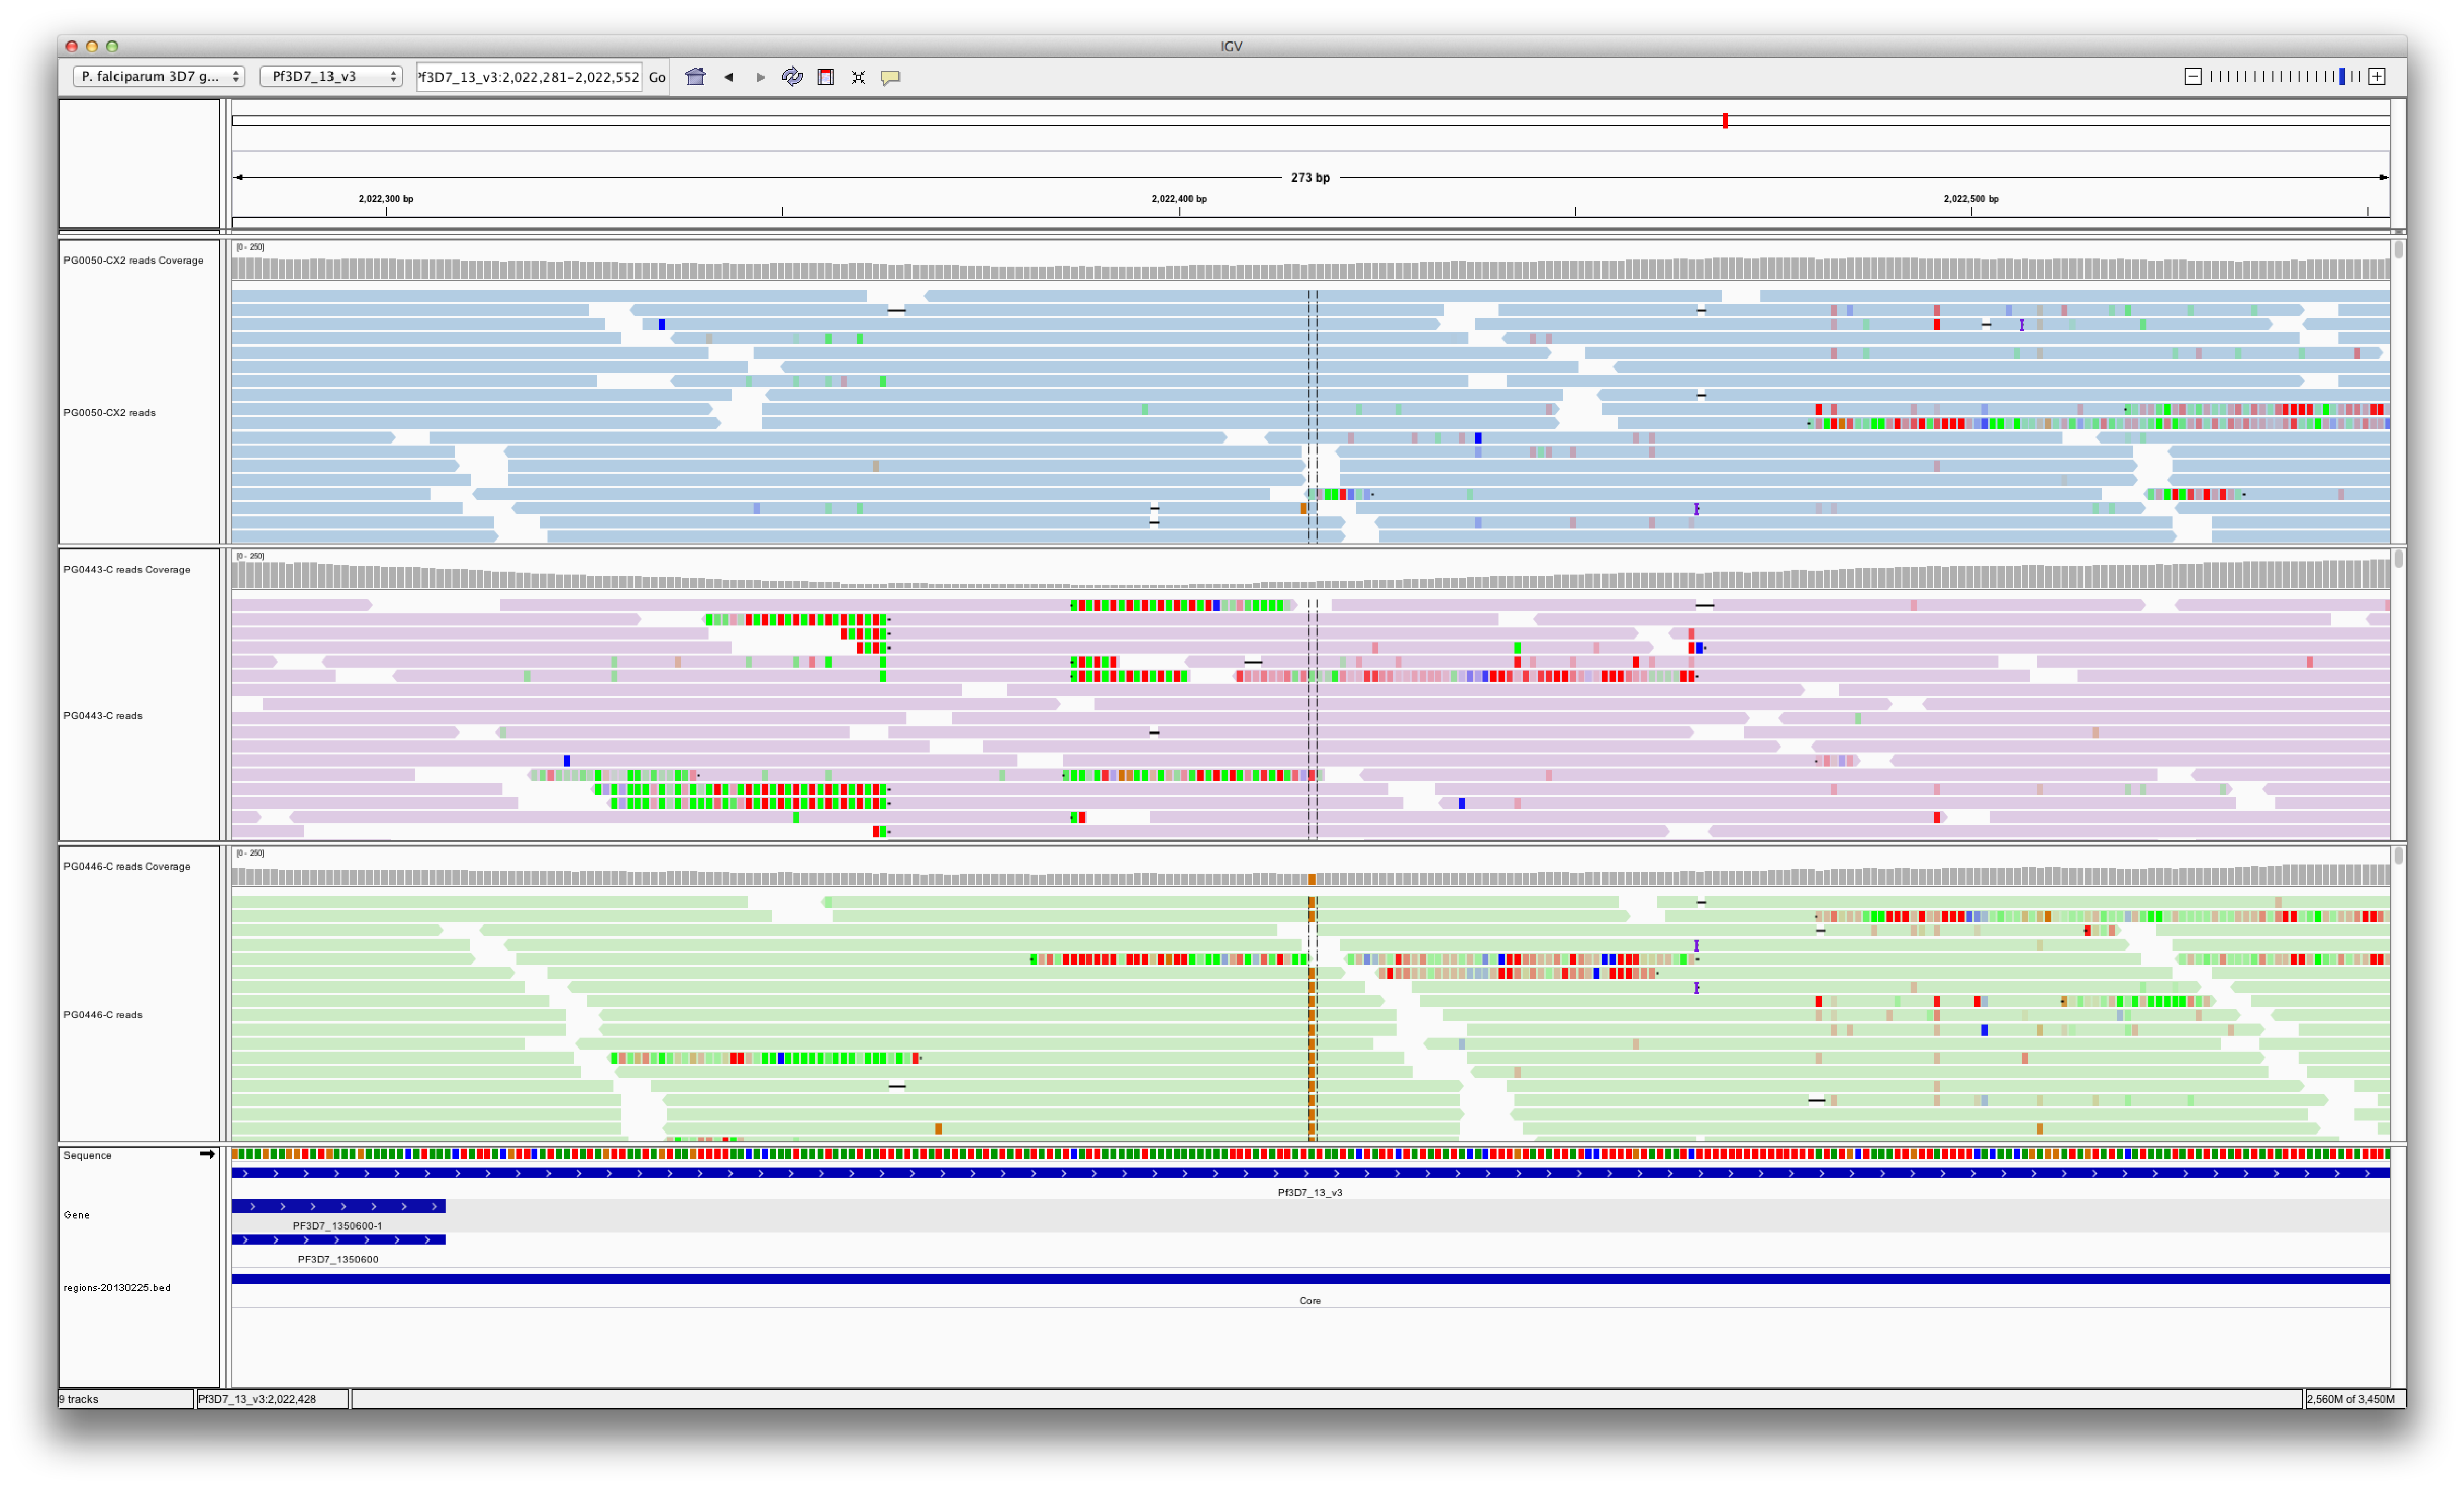
\includegraphics[width=\textwidth]{homlowcov}
  \caption{A validated \textit{de novo} SNP, recovered in the child amidst a great deal of sequencing error.  Top panel: PG0443-C (803).  Middle panel: PG0050-CX2 (GB4).  Lower panel: PG0446-C (child).}
  \label{fig:homlowcov}
\end{sidewaysfigure}

\begin{sidewaysfigure}[h!]
  \centering
    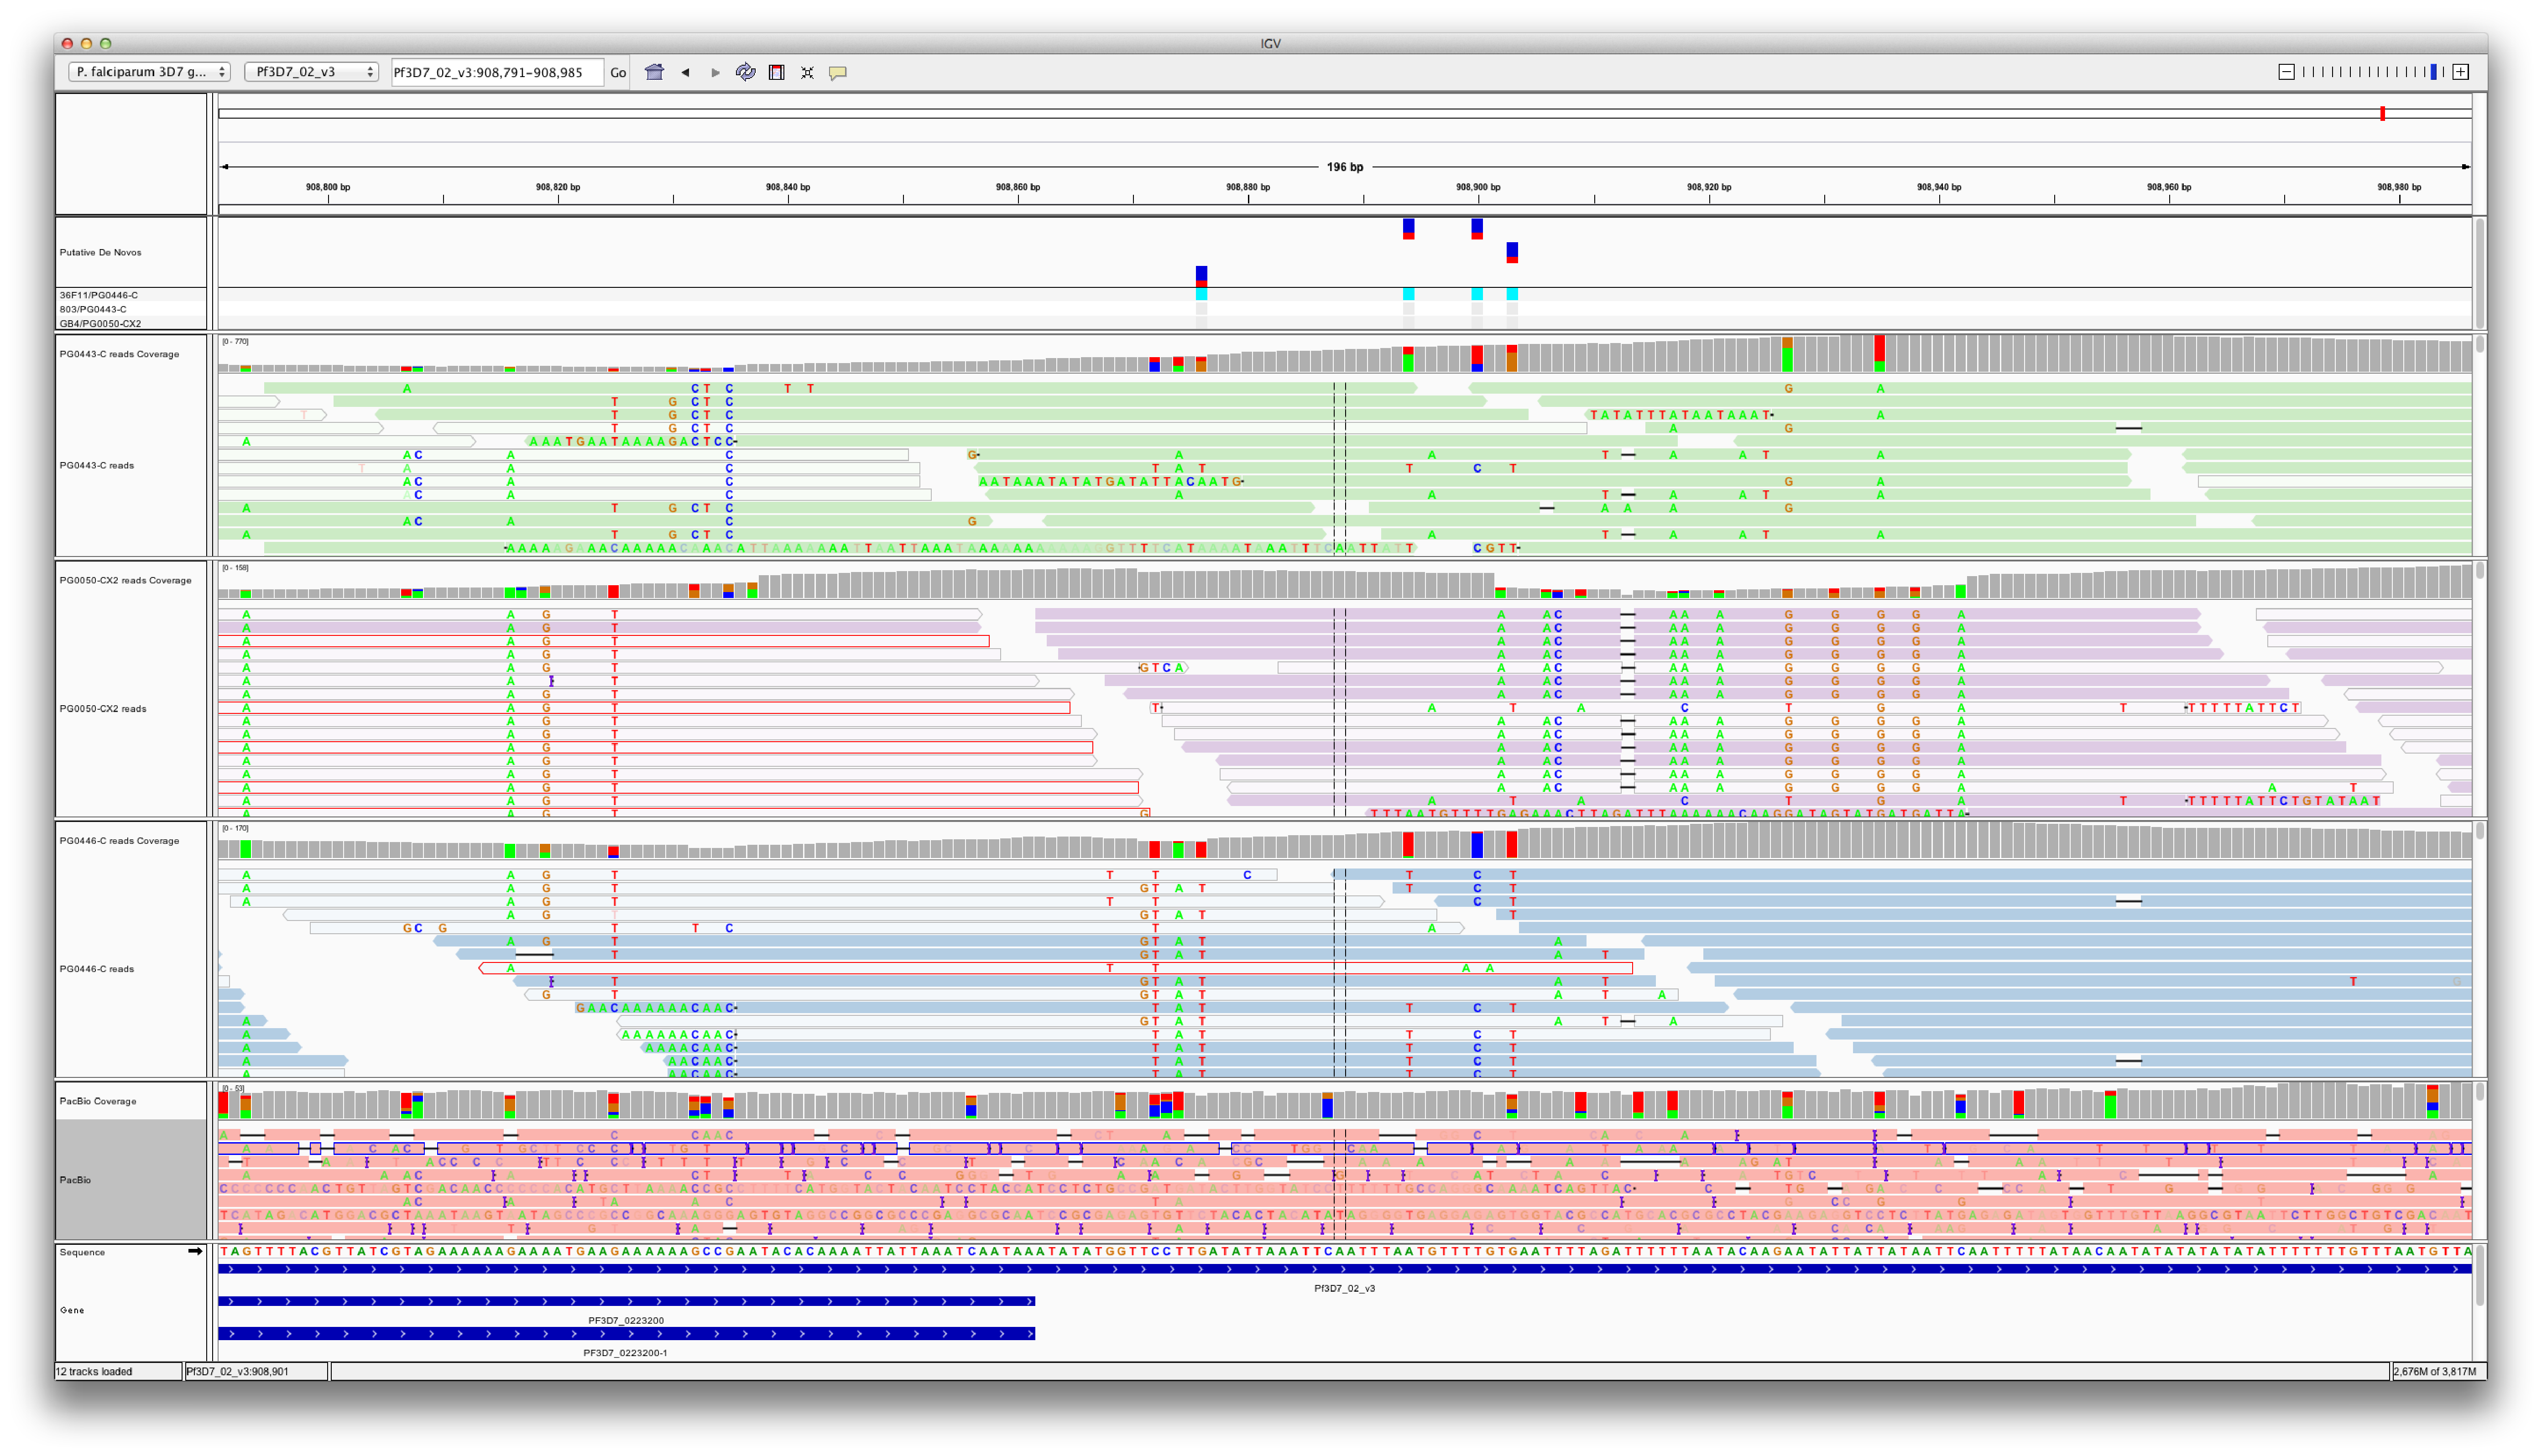
\includegraphics[width=\textwidth]{lotsosnps}
  \caption{False-positive \textit{de novo} variants in the 3' subtelomeric region of chromosome $2$.  Top panel: positions of the called variants in the reference-based analysis.  Second panel: PG0443-C (803).  Third: PG0050-CX2 (GB4).  Fourth: PG0446-C (child).  Fifth: Uncorrected PacBio reads from PG0446-C.  Bottom: gene model track from PlasmoDB $9.0$.  Stacked barplots above tracks indicate the proportion of reads supporting each allele.  Reads with ambiguous alignments are displayed in a lighter shade.}
  \label{fig:lotsosnps}
\end{sidewaysfigure}

\section{\textit{De novo} mutations in a single 3D7xHB3 sample}

\subsection{List of mutations}

A single validation sample is limited in its ability to inform us on the efficacy of the graphical variant calling approach, particularly as it apparently lacks an NAHR or other complex event for us to inspect.  We thus turned our attention to a single sample from the $3D7xHB3$ cross: PG0063-C.  This sample is known to harbor an NAHR event between two \textit{var} genes: $PF3D7\_0100100$ (situated in the 5' subtelomere of chromosome $1$), and $PF3D7\_0223500$ (the 3' subtelomere of chromosome $2$).  Their validated presence in PG0063-C makes this sample a particularly useful test sample for examination.

Applying our novel kmer identification software (and the new filters described above), we identified $314$ novel kmers corresponding to $77$ putative events.  Post-calling filtration brought this list down to $7$ events, described in Table \ref{tbl:callsPG0063C}.  These events are annotated with the locus, the haplotypic background of the variant, variant type, closest gene (and the associated product), and whether the variant falls within the MalariaGen variant calling exclusion mask.  The variants can be seen in their genomic context in Figure \ref{fig:circosPG0063C}.  

\begin{landscape}
\begin{table}[]
\centering
\caption{\textit{De novo} variants in 3D7xHB3 progeny, PG0063-C}
\label{tbl:callsPG0063C}
\begin{tabular}{@{}lllllll@{}}
\toprule
       & locus                & background &  event    &  closest gene                   &  product           &  within mask  \\
\midrule
1 (a)  & 1:27,780             & 3D7        &  SNP      &  PF3D7\_0100100                 &  PfEMP1 (var)       & yes          \\
1 (b)  & 1:27,782             & 3D7        &  MNP      &  PF3D7\_0100100                 &  PfEMP1 (var)       & yes          \\
1 (c)  & 1:27,854             & 3D7        &  MNP      &  PF3D7\_0100100                 &  PfEMP1 (var)       & yes          \\
1 (d)  & 1:29,441;2:923,083   & 3D7        &  NAHR     &  PF3D7\_0100100;PF3D7\_0223500  &  PfEMP1 (var)       & yes          \\
1 (e)  & 2:923,083;8:21,877   & 3D7        &  NAHR     &  PF3D7\_0223500;PF3D7\_0800100  &  PfEMP1 (var)       & yes          \\
1 (f)  & 8:21,877;1:30,087    & 3D7        &  NAHR     &  PF3D7\_0800100;PF3D7\_0100100  &  PfEMP1 (var)       & yes          \\
1 (g)  & 2:925,756;1:27,374   & 3D7        &  unknown  &  PF3D7\_0100100;PF3D7\_0223500  &  PfEMP1 (var)       & yes          \\
1 (h)  & 2:919,850            & 3D7        &  SNP      &  PF3D7\_0223500                 &  PfEMP1 (var)       & yes          \\
2      & 2:394,194            & HB3        &  unknown  &  PF3D7\_0209600                 &  transporter        & no           \\
3      & 4:568,395            & 3D7        &  SNP      &  PF3D7\_0412700                 &  PfEMP1 (var)       & yes          \\
4      & 4:568,401            & 3D7        &  SNP      &  PF3D7\_0412700                 &  PfEMP1 (var)       & yes          \\
\bottomrule
\end{tabular}
\end{table}
\end{landscape}

\begin{figure}[h!]
  \centering
    \includegraphics[width=\textwidth]{{PG0063-C.ERR019060.circos.edr}.png}
  \caption{Circos visualization of all \textit{de novo} mutations in PG0063-C, positioned on the reference sequence (outer ring), aligned maternal assembly (middle), and aligned paternal assembly (inner).  Unplaced parental contigs are concatenated and placed in the "U" pseudochromosome.  Each parental ring is annotated with a sequence compressibility score for every $2,500$ bp shown above their ideograms, while the reference ring is annotated with mean read coverage per $2,500$ bp.  Within the reference ideogram, all reference-based variant calls made in this sample from the MalariaGen project are shown, color-coded to reflect their parentage.  Regions that were masked out of MalariaGen's variant calling process are shown as grey bars.  Variants are shown as glyphs below the parental ideograms, shape-coded for type (small circle: unknown, large circle: SNP, triangle: indel, square: MNP, diamond: NAHR event).  The color and positioning of the glyph reflects the haplotypic background upon which the event occurred.  Interchromosomal structural variation and gene-conversion events are additionally denoted as arcs linking the relevant parts of the genome.  The closest gene to the event is reported in black if the mutation falls within the gene and as grey if it falls outside the gene.}
  \label{fig:circosPG0063C}
\end{figure}

There are several noteworthy features of Table \ref{tbl:callsPG0063C} and Figure \ref{fig:circosPG0063C}.  First, we discover a variety of event types, including SNPs (depicted in the plot with large circles), indels (triangles), multi-nucleotide polymorphisms (squares), and NAHR events (diamonds).  Few events could not be typed (small circles).

Second, we are able to localize all mutational events within the parental genomes, even if the precise nature of the event could not be ascertained.  Here, we benefit from aligning the parental sequences rather than the child's sequence or short $76$ bp reads.  The parental sequences are often be longer than a read length, and should obviously match the parental genomes more closely.  This provides the alignment software more context and less variation with which to determine an appropriate home for the mutation.

Third, we are able to identify interchromosomal exchanges, including the known NAHR event between PF3D7\_0100100 on the 5' end of chromosome $1$ and PF3D7\_0223500 on the 3' end of chromosome $2$\cite{Anonymous:2013hi}.  Curiously, there is another apparent interchromosomal exchange involving these two \textit{var} genes and one on chromosomes $8$.  No such recombination is reported in the literature, and the event is supported by a very short contig aligned to chromosome $8$ ($< 50$ bp).  While it is conceivable that the NAHR machinery may switch templates to potentially involve content from a third chromosome, it is more plausible that the recombination process gave rise to a short region of low-complexity sequence that happens to occur elsewhere in the genome.

Fourth, we are able to detect mutations that occur in regions of the reference genome typically ignored in reference-based analyses.  MalariaGen delibrately excluded a number of regions from processing, including repetitive regions (often telomeric, centromeric, or pericentromeric regions) as short reads could often not be aligned in long repetitive regions with confidence.  It also excluded hypervariable regions (typically subtelomeric) as population diversity was too high to yield confident results in the reference-based analysis.  As we are comparing each sample to a parental graph rather than a reference sequence that is an undetermined number of generations removed, our graphical approach can reconstruct and localize these events.

Fifth, our calls in this sample appear overwhelmingly concentrated in or near antigenic genes ($8$/$9$).  Such a skew is unusual, especially given the fact that our algorithm is hypothesis-free and is not biased towards processing any particular region of the genome.

Sixth, the call rate is reasonably low; $9$ events in this sample total.  However, the first several events in the table appear to take place in the same \textit{var} genes.  Presumably, these events are all part of the single NAHR event.  Counted together, the revised \textit{de novo} mutation count is $4$.  Both are consistent with the expectation from the validation data that \textit{de novo} mutations should be rare.

Subtelomeric regions (and the antigenic genes contained within) are known to be high in repetitive sequence.  To visualize the potential relationship between sequence content and variant location, we examined a number of different sequence properties.  Shown in Figure \ref{fig:circosPG0063C} above each parental assembly track is one of these metrics: the sequence compression ratio.  Many of our DNM calls appear to follow closely with spikes in the local sequence compressibility measure.  Quite often these spikes correspond with being in a masked repetitive region.

\subsection{Manual examination of all \textit{de novo} mutations}

To establish the veracity of these calls, we manually examined all events in Table \ref{tbl:callsPG0063C} in IGV and our custom graph viewing software.

\subsubsection{Event $1$ (a-h): NAHR}

The first event in Table \ref{tbl:callsPG0063C} appears to be an NAHR event.  Unfortunately, short reads are insufficient to capture the entire event in a single contig.  Instead, we see pieces of the chromosomal exchange manifest as a series of SNPs, MNPs, and longer sequences that co-localize disparate regions of the genome onto a single contig.

The first three variants ($1a-c$: a SNP and two MNPs), are depicted in Figure \ref{fig:event1a-c}.  Upon initial inspection, it is not immediatley obvious that the child's reads are sampled from the maternal or paternal haplotypes at all.  Many apparent variants from the HB3 parent are not present in the child.  Several loci appear to be polymorphic.  It is tempting to conclude that the results are indicative of sequencing error or myriad mutational events sustained in mitosis.  However, given the repetitive nature of the locus, the presence of ambiguously aligned reads (shown in translucent colors), and reads with several mismatches, it is more likely that many reads sampled from similar haplotypes are simply misaligned to the sole copy in the reference sequence.

\begin{sidewaysfigure}[h!]
  \centering
    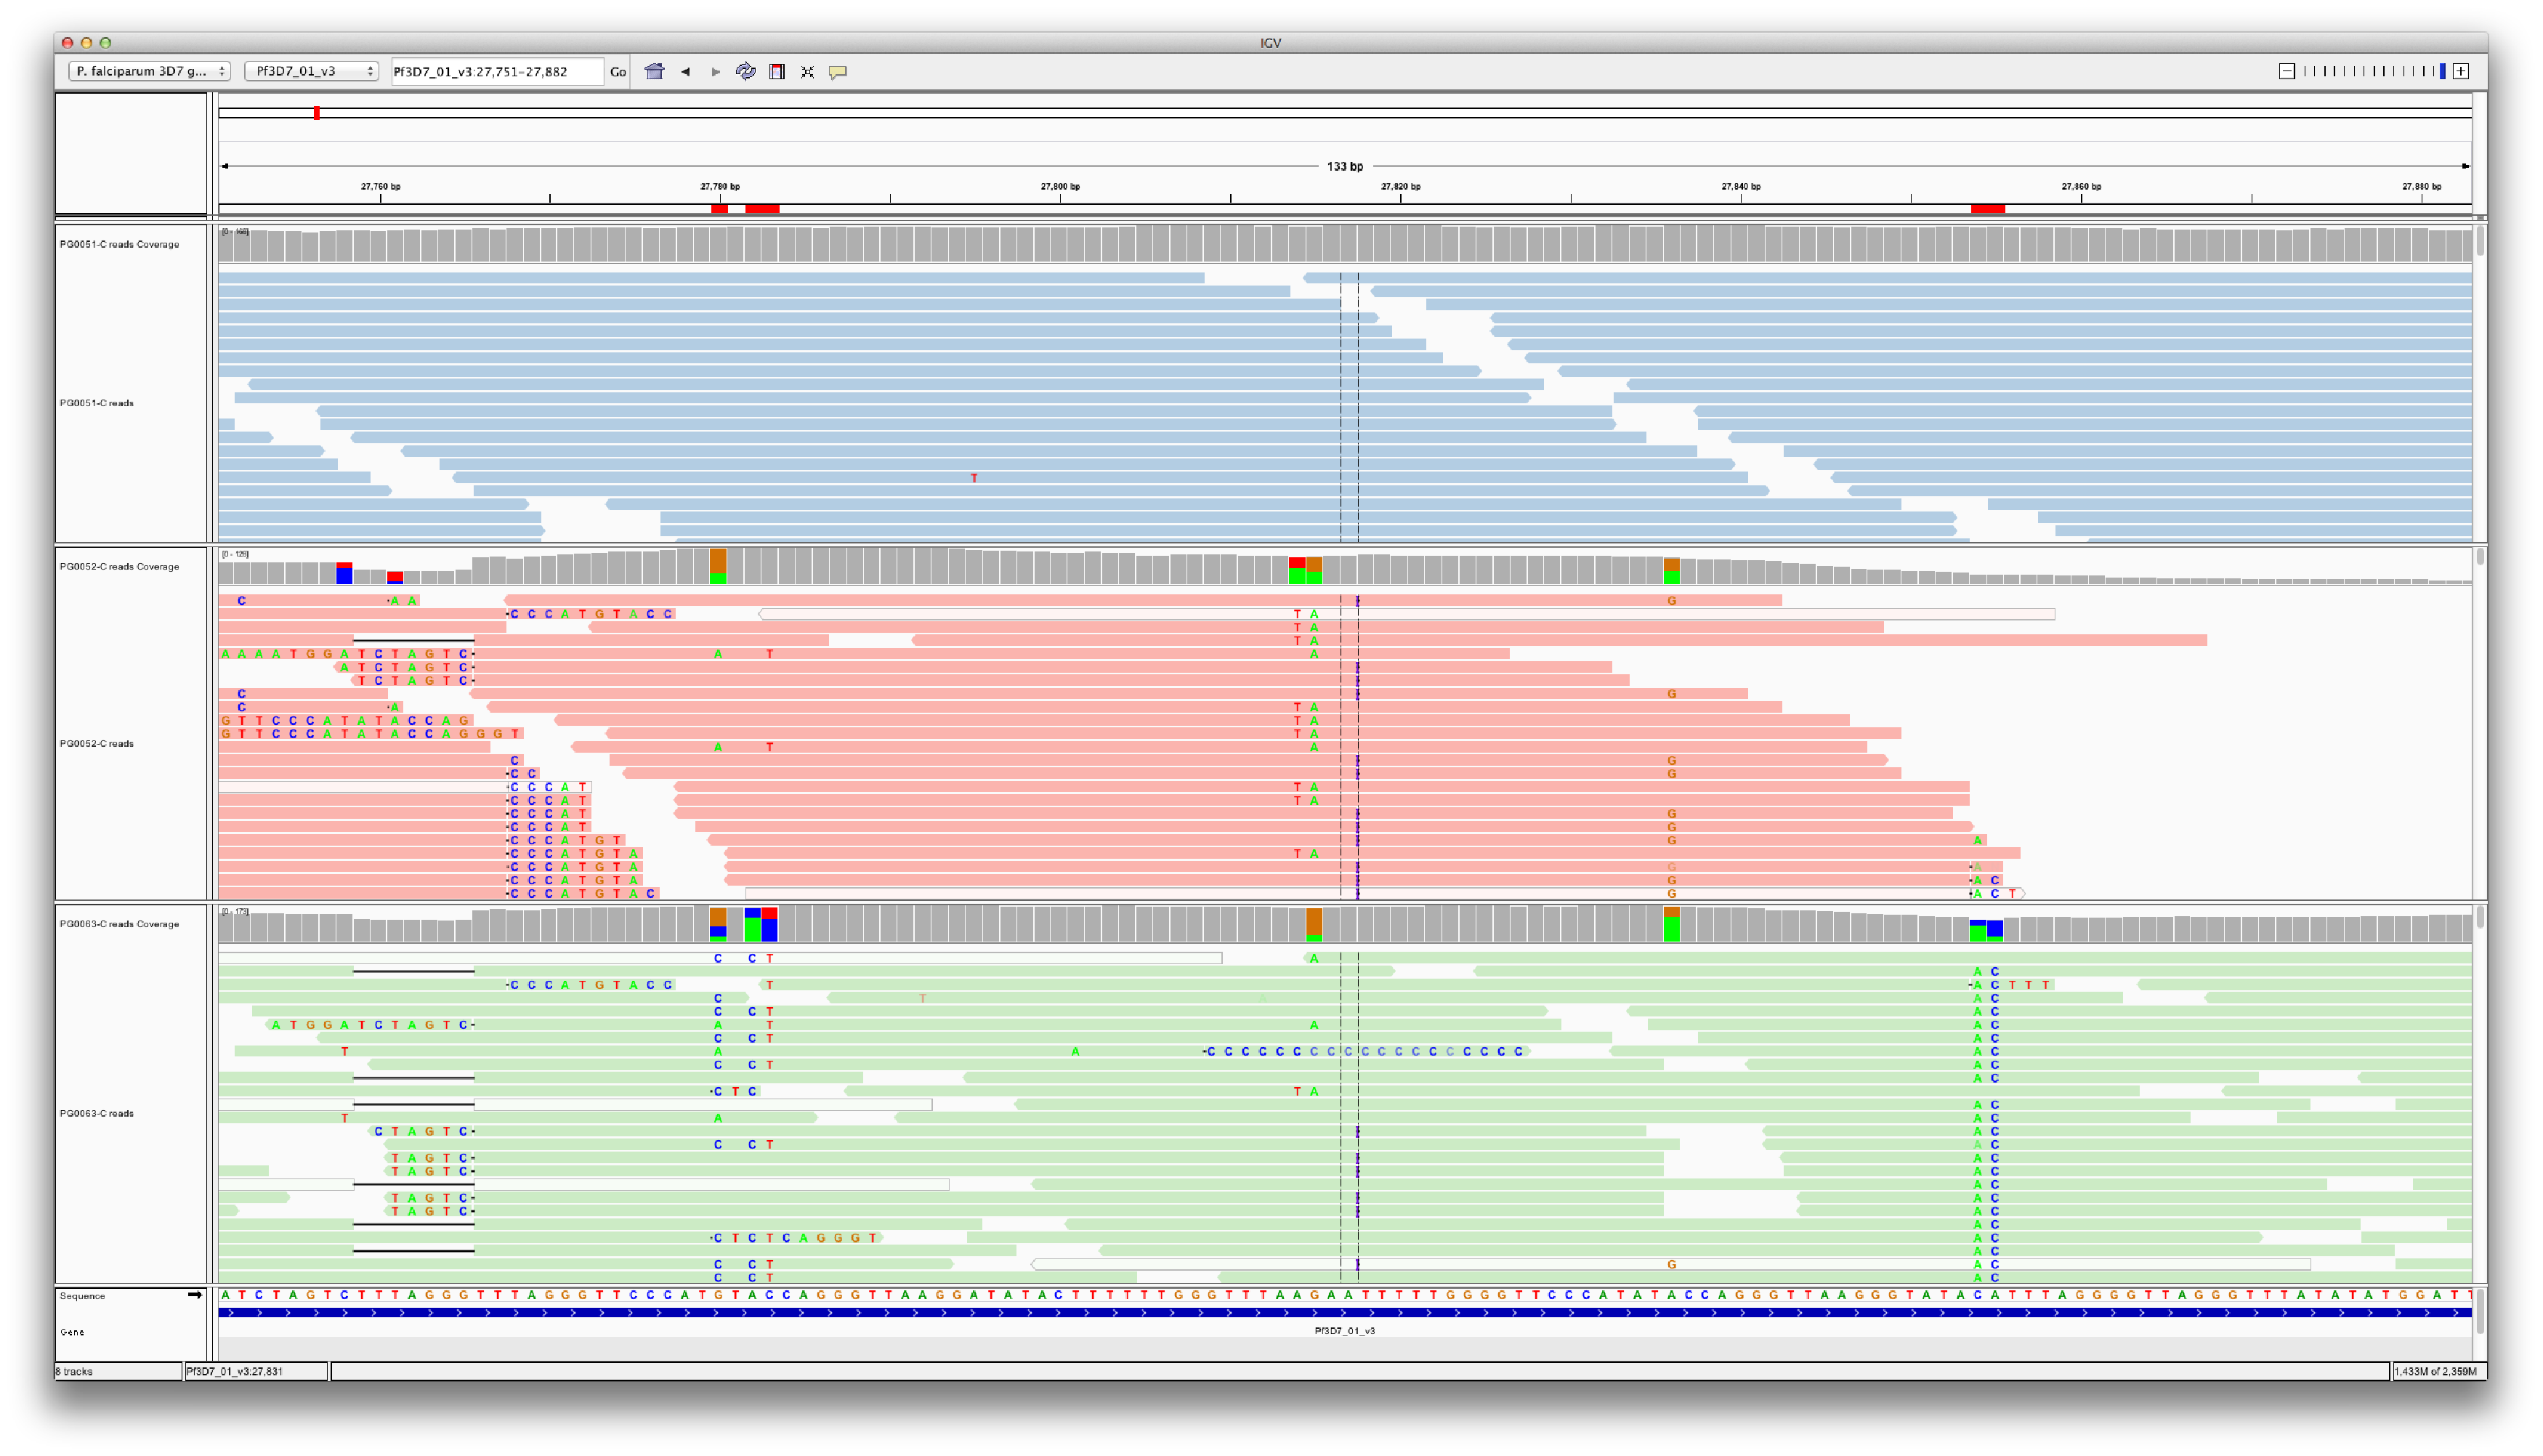
\includegraphics[width=\textwidth]{event1a-c}
  \caption{IGV screenshot of SNP and two MNPs: three apparent \textit{de novo} mutations within a much larger NAHR event.  Top panel: 3D7 parent.  Middle panel: HB3 parent.  Lower panel: PG0063-C child.  Variant positions are shown as red blocks at the top of the three panels below the genome position track.  Stacked barplots above variant positions indicate the proportion of bases supporting an alternate allele to the reference.}
  \label{fig:event1a-c}
\end{sidewaysfigure}

The local subgraph for these events, shown in Figure \ref{fig:event1a-cgraph}, exhibits a complicated structure containing several tendrils to homologous (but irrelevant) regions of the genome.  Despite this complexity, two bubble motifs (drawn with thicker lines) can clearly be observed, encapsulating the first SNP/MNP\footnote{As these events are separated by less than a kmer length, they present as a single bubble.} and second MNP.  Inspection of individual vertices in the event reveals all kmers to be of nominal coverage ($> 40x$), and the subgraph itself is devoid of any suspicious kmers (contaminants, exceedingly low-coverage sequence, or dirty kmers) that would be suggestive of error.

\begin{figure}[h!]
  \centering
    \includegraphics[width=\textwidth]{{event1a-c.graph}.pdf}
  \caption{IGV screenshot of SNP and two MNPs: three apparent \textit{de novo} mutations within a much larger NAHR event.  Top panel: 3D7 parent.  Middle panel: HB3 parent.  Lower panel: PG0063-C child.  Variant positions are shown as red blocks at the top of the three panels below the genome position track.  Stacked barplots above variant positions indicate the proportion of bases supporting an alternate allele to the reference.}
  \label{fig:event1a-cgraph}
\end{figure}

The next four events capture the NAHR event itself and are displayed in Figure \ref{fig:event1d-h}.  The graphical view shows a very simple structure, unmarred by indications of sequencing error.  Starting from the upper right, the child and 3D7 assemblies track along chromosome $1$ until the child's assembly forks off, apparently passing through a few kmers from chromosome $8$, rejoining at chromosome $2$.  Meanwhile, the 3D7 genome continues to track along chromosome $1$ until it rejoins a region of the child's assembly (towards the bottom of the image).  Here, 3D7 and the child fork again, with the child's assembly connecting again to chromosome $2$.  The IGV panels show the reads aligned to these regions of the 3D7 reference genome.  In the $b$ panel (shoing the $5'$ end of chromosome $1$, the reads appear to be sampled largely from the 3D7 parent until an abrupt change midway through the track (denoted by the red bar).  Similarly, the $c$ panel shows a region on chromosome $2$ that supports the 3D7 haplotype over a window substantially longer than a read length ($300$ bp).

\begin{sidewaysfigure}[h!]
  \centering
    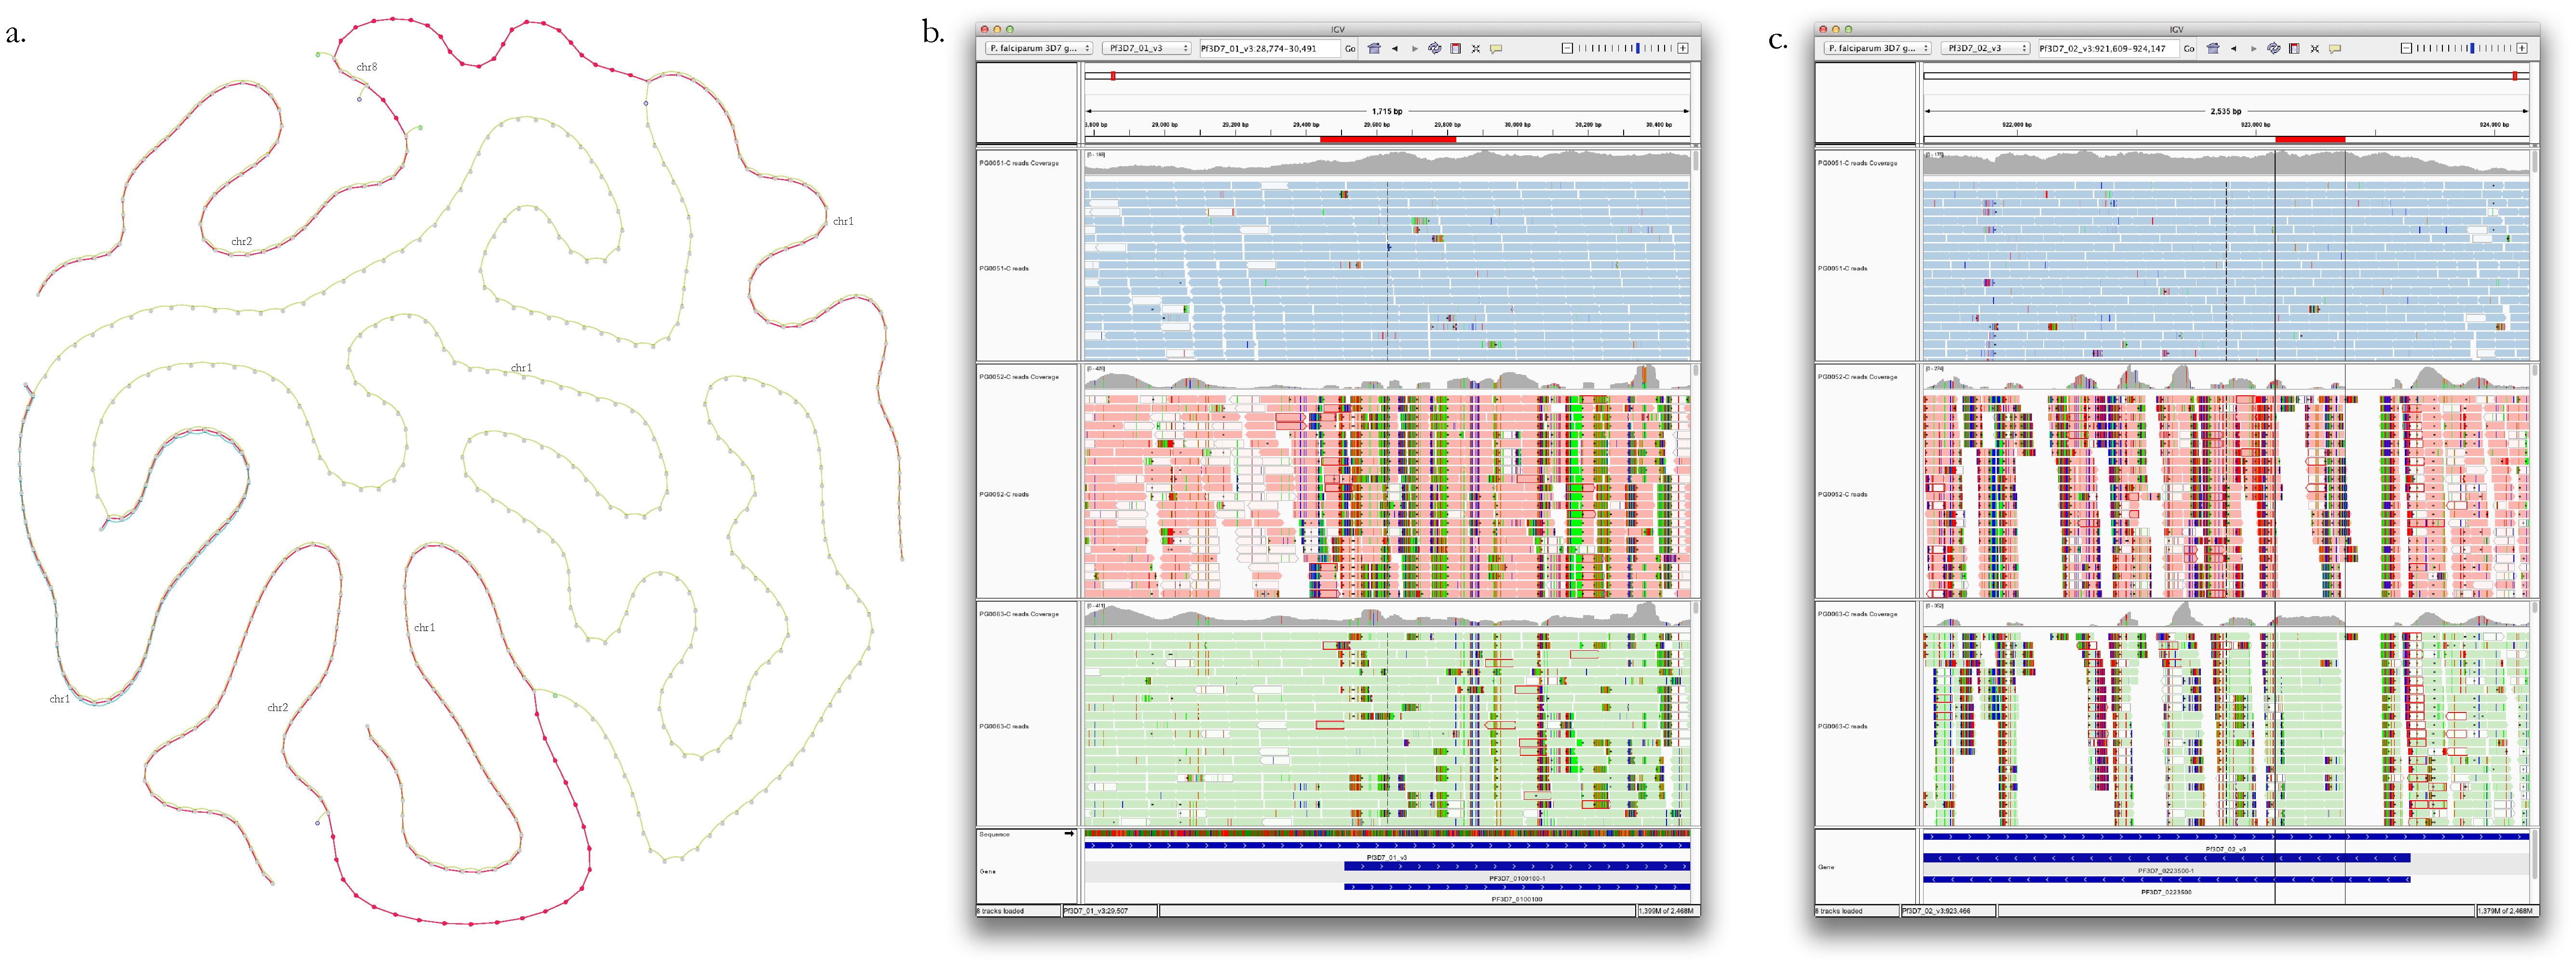
\includegraphics[width=\textwidth]{event1d-h}
  \caption{A NAHR event.  a. Graphical view of the exchange; chromosome of origin specified for various regions.  b. IGV screenshot for 3D7 (top), HB3 (middle), and PG0063-C (child) on the chromosome $1$ region of the event.  c. IGV screenshot of the chromosome $2$ region of the event.}
  \label{fig:event1d-h}
\end{sidewaysfigure}

The last mutation seemingly associated with the NAHR event is a single SNP; the context is shown in Figure \ref{fig:funnysnp}.  A naive analysis would not assign \textit{de novo} status to such an event as there appears to be some evidence for this allele in the HB3 parent.  However, the left and right sections of the HB3 reads flanking the putative variant exhibit an extraordinary number of mismatches and are clipped off in the alignment.  A small number of reads have mapping quality $0$, indicating that the aligner had no confidence in their placement.  While the 3D7 parent and the child are covered over this region to $> 150x$, the HB3 sample is only covered to $20x$, with many apparent holes in the coverage across the $200$ bp region shown.  Finally, the child's alignments are very clean across this region: no mismatches, no clipped reads, and consistent coverage.  It is likely that the HB3 alignments are in error - a homologous region from another \textit{var} gene have landed here because the proper haplotype is not represented in the reference.  Our graphical method detects the mutation on the correct haplotypic background and calls it accordingly.

\begin{sidewaysfigure}[h!]
  \centering
    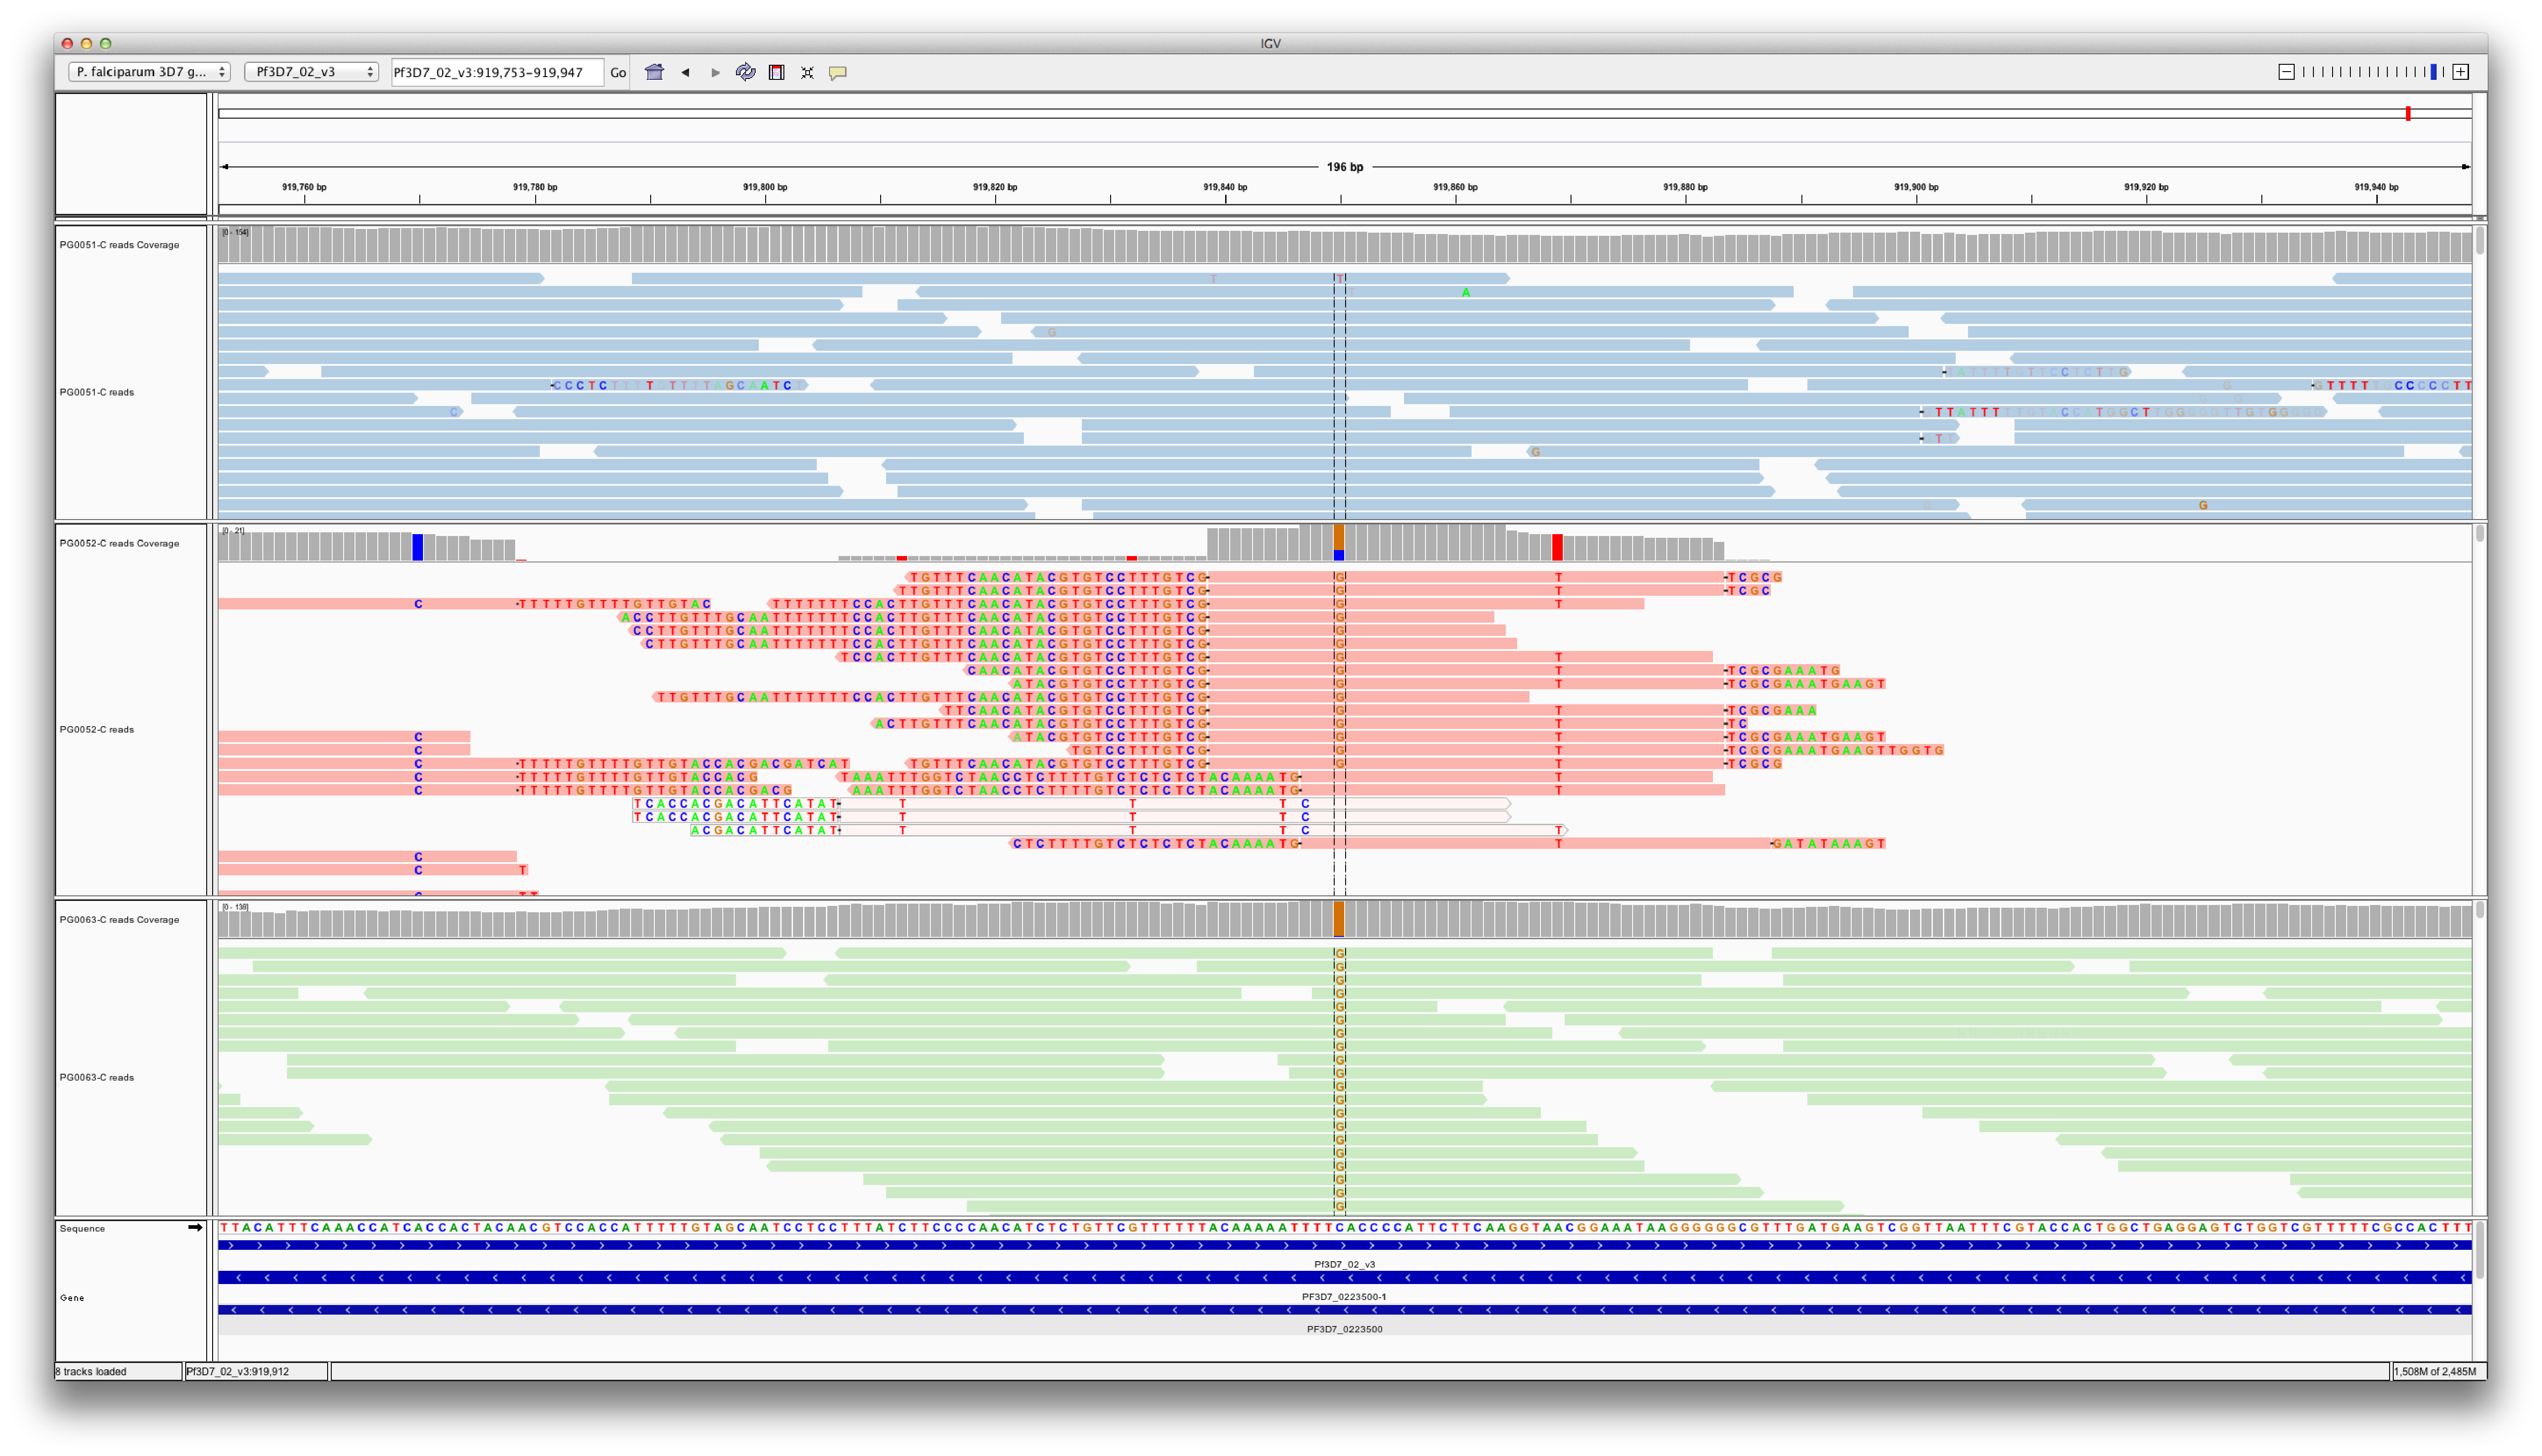
\includegraphics[width=\textwidth]{funnysnp}
  \caption{A \textit{de novo} SNP in a \textit{var} on the 3D7 haplotypic background.  Top panel: 3D7.  Middle: HB3.  Lower: PG0063-C child.}
  \label{fig:funnysnp}
\end{sidewaysfigure}

\subsubsection{Event $2$: unknown}

\begin{figure}[h!]
  \centering
    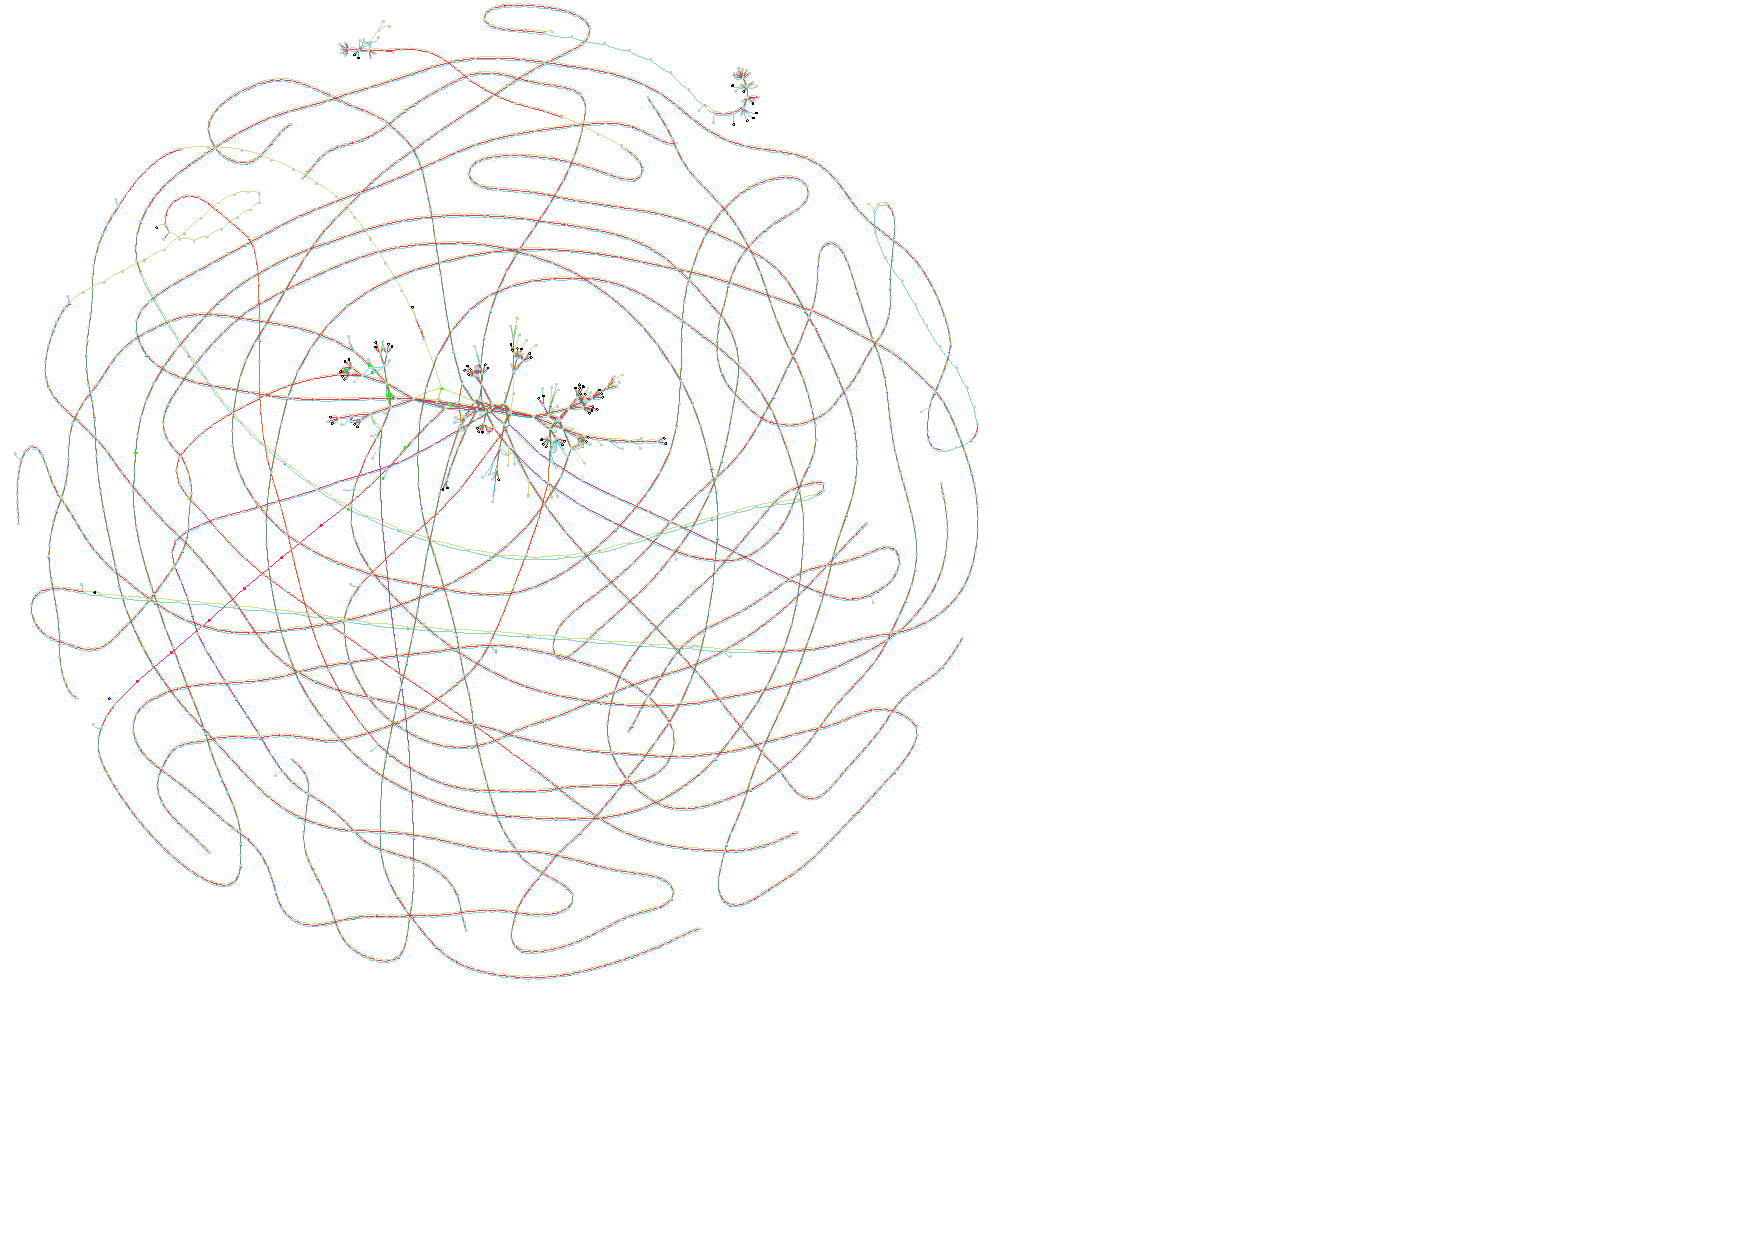
\includegraphics[width=\textwidth]{tangle}
  \caption{A graph "tangle": a region of the graph where the in/out degree of vertices within a small radius sharply increases, resulting from attempting to traverse a low-complexity region of the genome.}
  \label{fig:tangle}
\end{figure}

Event $2$ is an unknown event, seemingly localized to the $5'$ telomere of chromosome $2$.  However, examination of the subgraph (Figure \ref{fig:tangle} reveals the event in question likely stems from a graphical "tangle": a region of the graph where long, uninterrupted, singly-connected regions of the graph collapse into a messy structure wherein every vertex appears to connect to many others.  The IGV screenshot for this region (Figure \ref{fig:tangle.igv} shows a number of errorful reads spanning a homopolymer region.  If these results are due to a recurrent error by the sequencer (sometimes skipping one, two, or many bases), they may occur slightly differently between samples and often enough to produce enough kmers to overcome the novelty coverage thresholds.  This would give rise to a stretch of novel kmers near the low-complexity region that fails to resolve into a \textit{de novo} variant.

One can conceive of a few simple checks to remove these events from our callset (e.g. walking the graph within a certain radius to discover potential nearby tangles).  However, such regions may also be biologically interesting, potentially giving rise to small indels induced by DNA repair over those low-complexity sequences.  Unclassified events are not harmful to us, as they will not count in measures of SNP, MNP, indel, or NAHR event mutation rates.  They simply eat up novel kmers without assigning any identity to the kmers.  For these reasons, we have not made strong efforts to filter them out.

\begin{sidewaysfigure}[h!]
  \centering
    \includegraphics[width=\textwidth]{{tangle.igv}.pdf}
  \caption{A low-complexity region of the genome containing many reads with many apparent errors.}
  \label{fig:tangle.igv}
\end{sidewaysfigure}

\subsubsection{Events $3$ and $4$: two SNPs}

\begin{sidewaysfigure}[h!]
  \centering
    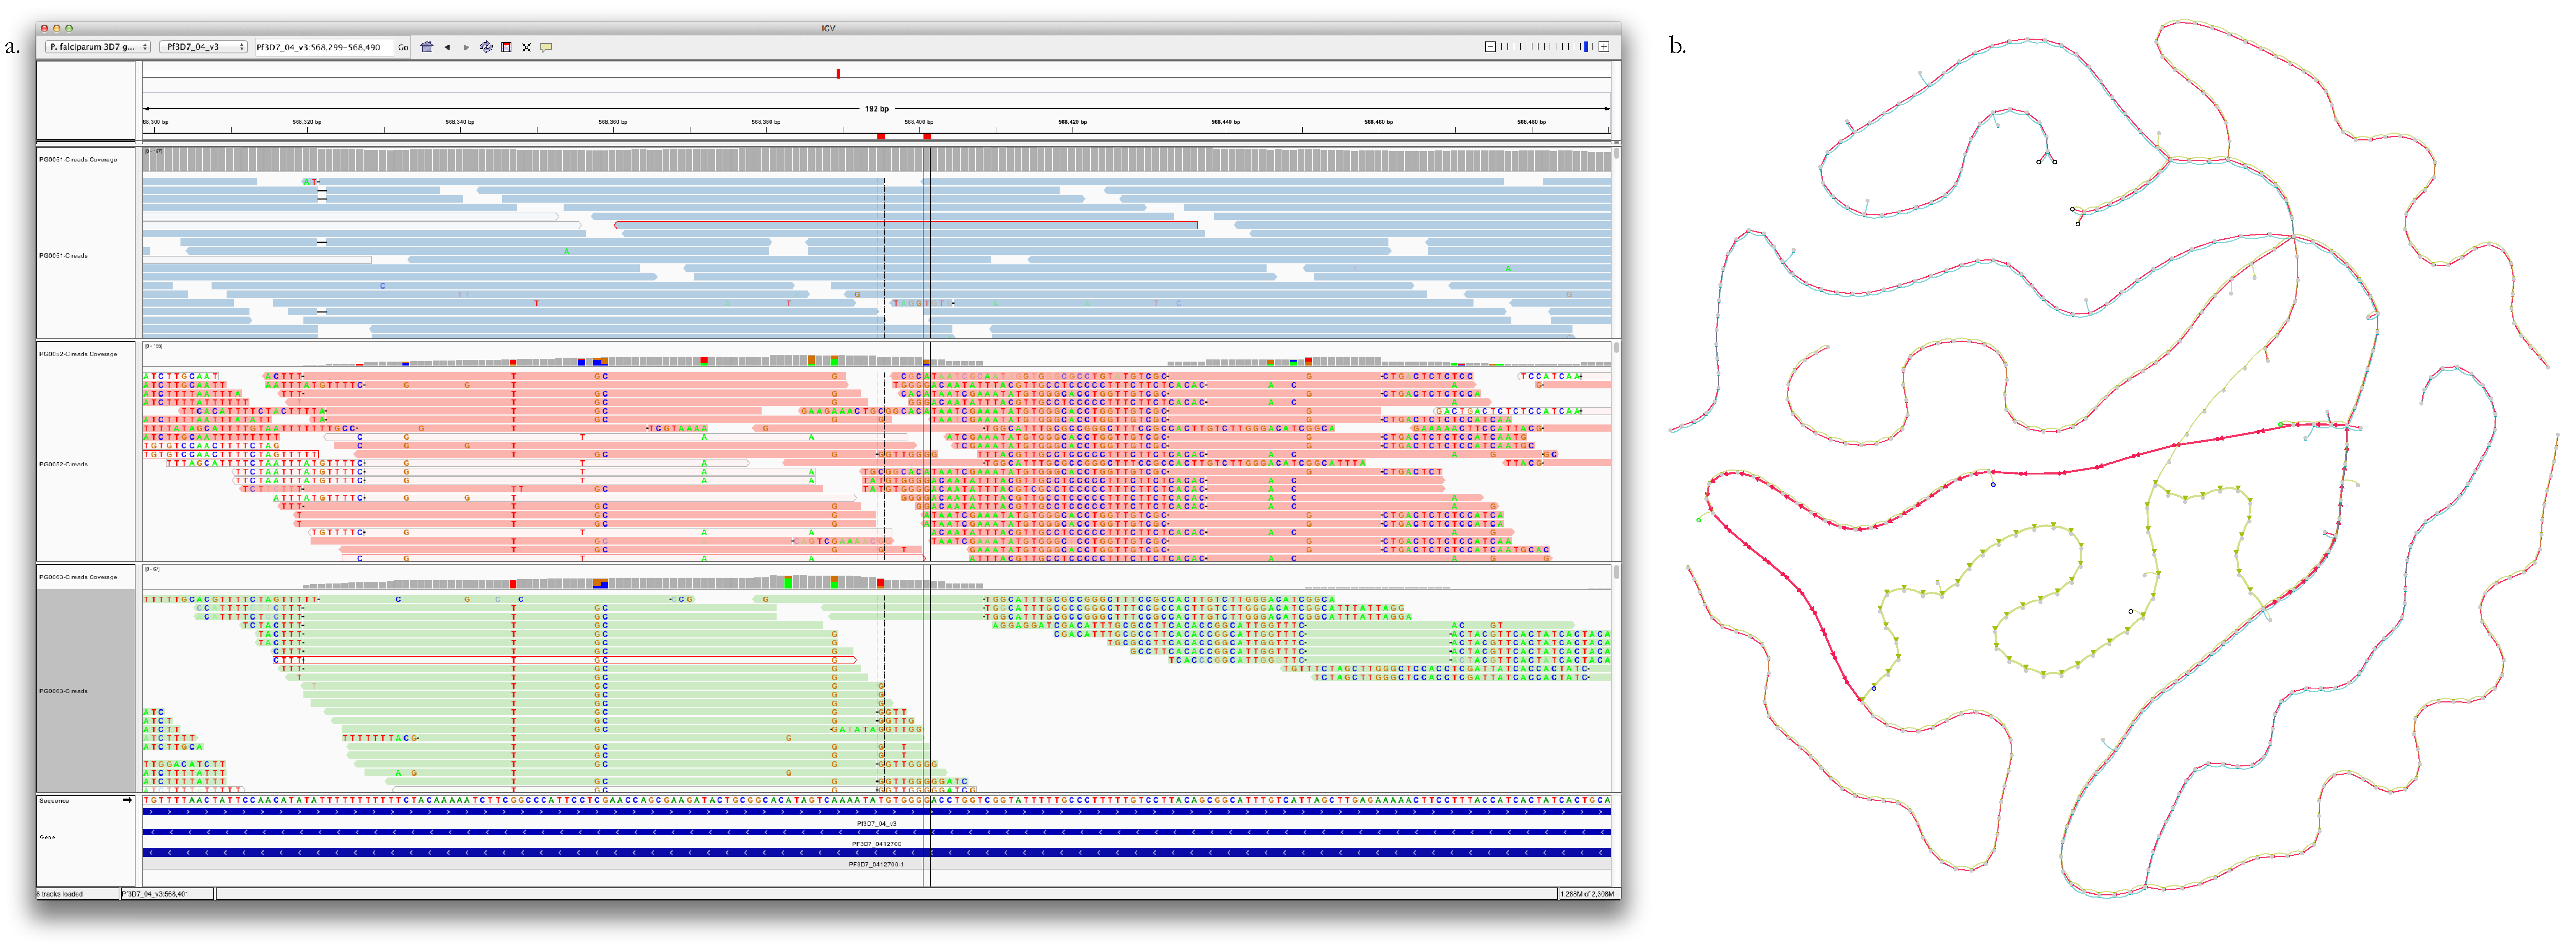
\includegraphics[width=\textwidth]{twosnps}
  \caption{Two SNPs, non-obvious from the alignments, but apparent in graph.  a. IGV screenshot of two \textit{de novo} SNPs in a \textit{var} gene.  b. Graphical view of the two SNPs.}
  \label{fig:twosnps}
\end{sidewaysfigure}

Figure \ref{fig:twosnps} show the last events in this sample, two SNPs set $5$ bp apart, and reveal an interesting limitation of our graphical approach.  While our alignments of the parental sequence suggest these events occur on chromosome $4$, no evidence for the events are found at that locus.  A BLAST search reveals the proper home (barring a single nucleotide) to be on chromosome $1$, within the PF3D7\_0100100 \textit{var} gene - the same gene involved in the NAHR event described above.  This locus is shown in Figure \ref{misplacedsnp}.  The misplacement of these events are likely due to an error in the reference sequence.  A single nucleotide error in the reference sequence prevents us from finding the true home of the kmers spanning the error.  By chance, those aberrant kmer exist elsewhere in the genome: a \textit{var} gene on chromosome $4$.  This misleads us into choosing the home on chromosome $1$ instead.  Thus, while the events are likely to be real, our placement is erroneous.

\begin{sidewaysfigure}[h!]
  \centering
    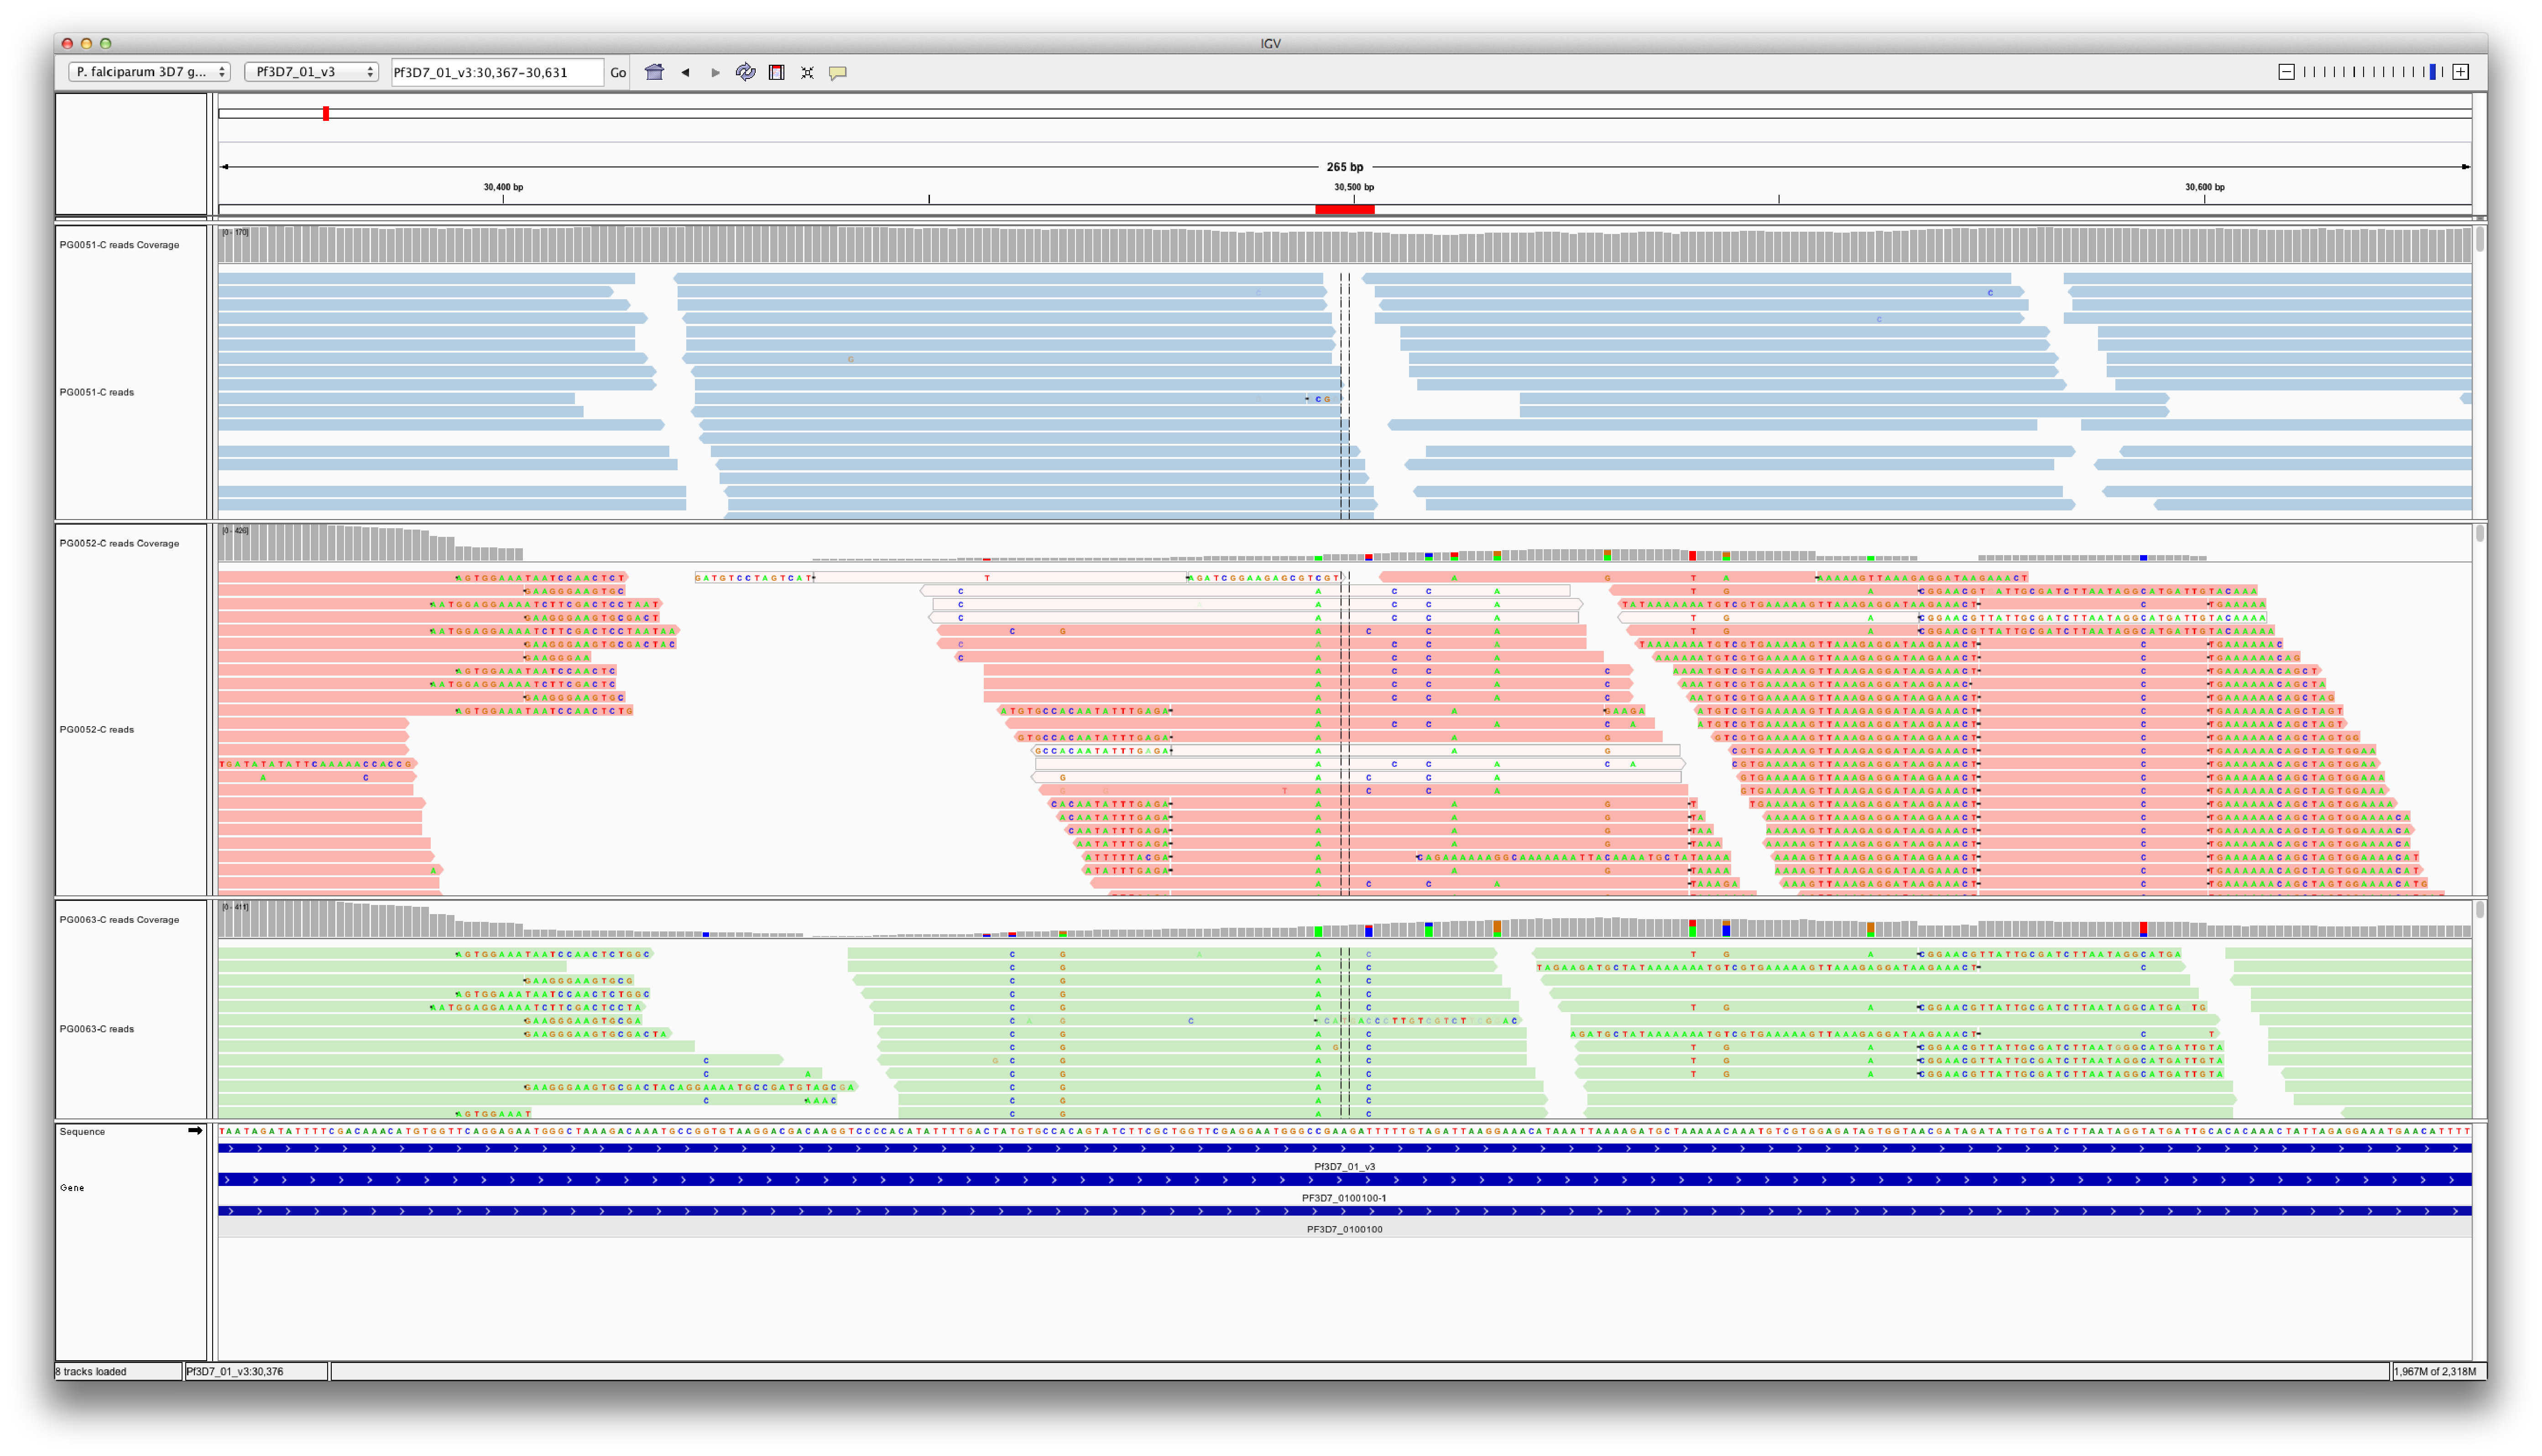
\includegraphics[width=\textwidth]{misplacedsnp}
  \caption{The true home of the aforementioned two SNPs.}
  \label{fig:misplacedsnp}
\end{sidewaysfigure}

\subsection{Rejected events}

Post-calling filters rejected nine putative \textit{de novo} events.  These events were rejected for a variety of reasons: either internal use of dirty kmers exceeded a maximum threshold of $10\%$ (5), the novel kmers were found at the extremeties of a graph with no apparent connection to any other part of the genome (2), or the contig failed to align to any part of the genome (2).  Most rejected events were of an "unknown" event type (no label could be reasonably assigned to the putative variant).  One was a potential recombination event, but upon inspection of the data in IGV, a recombination event is not readily apparent.

Events lacking alignments do not visualize well; there is nothing to display in IGV and the graph itself is non-descript (potentially an unrecognized contaminant).  An event with dirty kmers and an event with novel kmers without connection to the rest of the graph are shown in Figure \ref{fig:graphfilters}.  Notice that these filters are clearly not orthogonal; had the event with dirty kmers remained in consideration, it would have been flagged as a disconnected event as well.

\begin{figure}[h!]
  \centering
    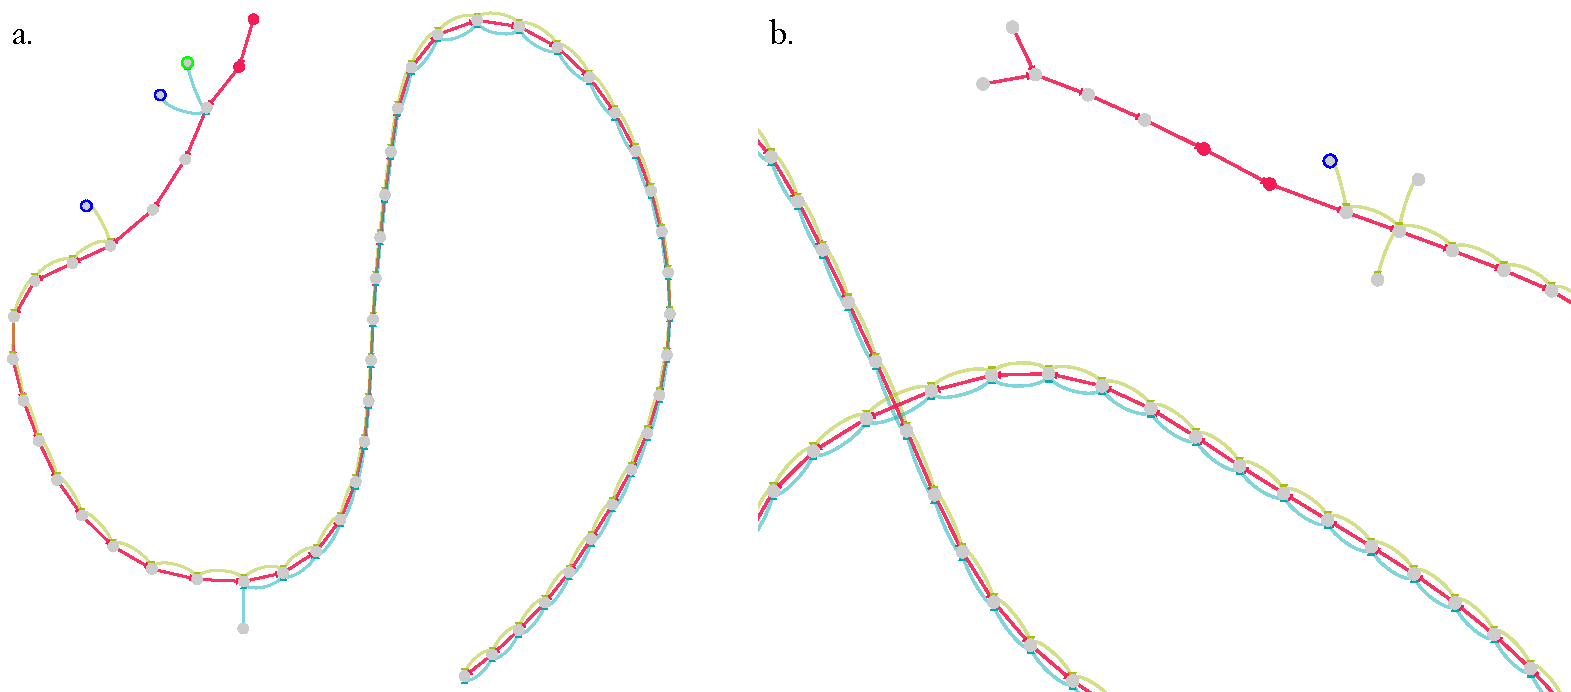
\includegraphics[width=\textwidth]{graphfilters}
  \caption{Graph motifs for discarded events.  a. Disconnected events: novel kmers that fail to link back to the genome.  b. "Dirty" events: the dirty kmers (shown in grey with red edges) make up more than $10\%$ of the novel kmers in the region.}
  \label{fig:graphfilters}
\end{figure}

\subsection{Novel kmer accounting}

\begin{figure}[h!]
  \centering
    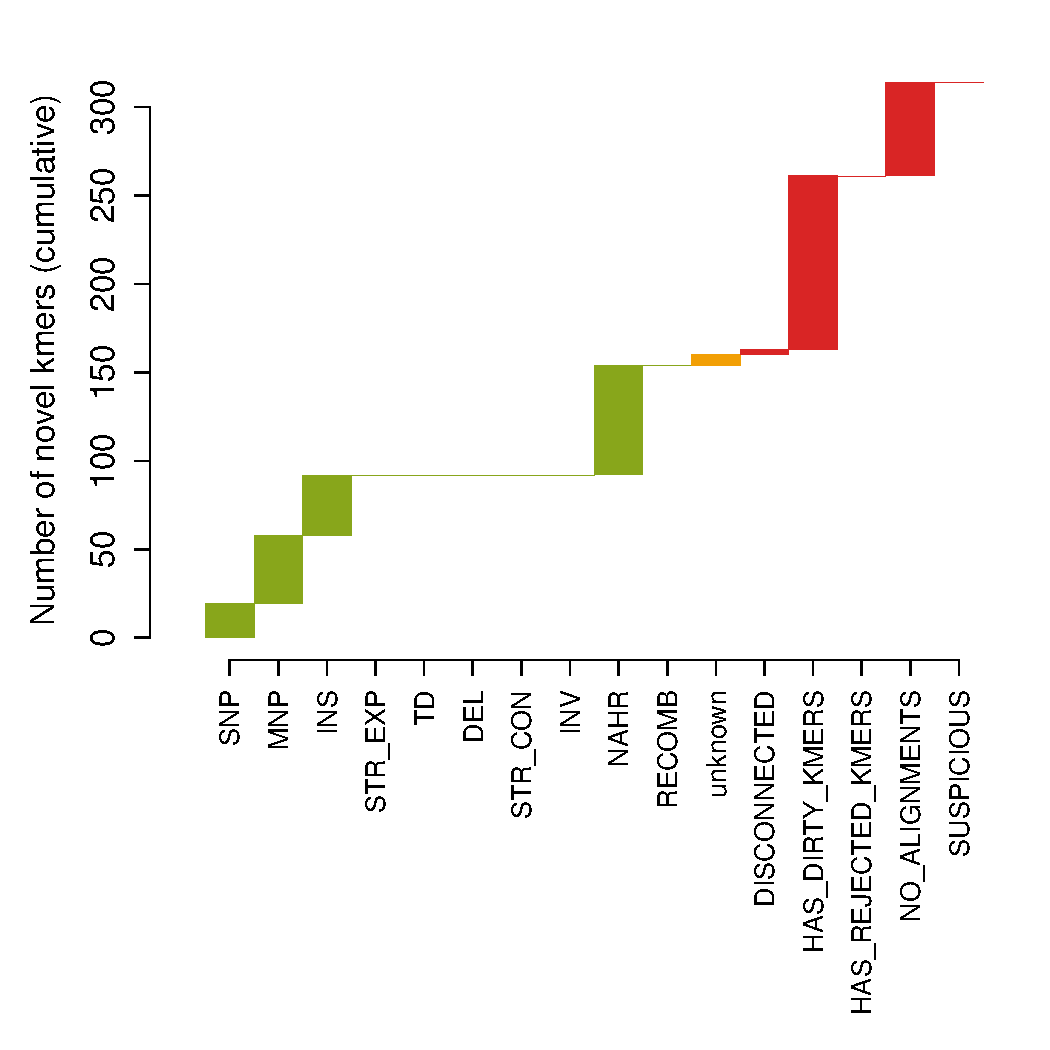
\includegraphics[width=0.7\textwidth]{accounting-1}
  \caption{Cumulative accounting of novel kmers and the mutation types to which they correspond.  Events passing filters are depicted in green.  Those failing filters are in red.}
  \label{fig:accounting}
\end{figure}

Figure \ref{fig:accounting} details the cumulative usage of novel kmers in the PG0063-C sample.  Of the $314$ novel kmers detected, $154$ were discarded as part of events suspected not to be true mutational events.  The remaining $160$ are present in mutational events passing filters.  $156/160$ ($97.5\%$) of novel kmers could be assigned to a definable mutational type.

\section{\textit{De novo} mutations in all crosses and samples}

\subsection{Novel kmer use}

\begin{figure}[h!]
  \centering
    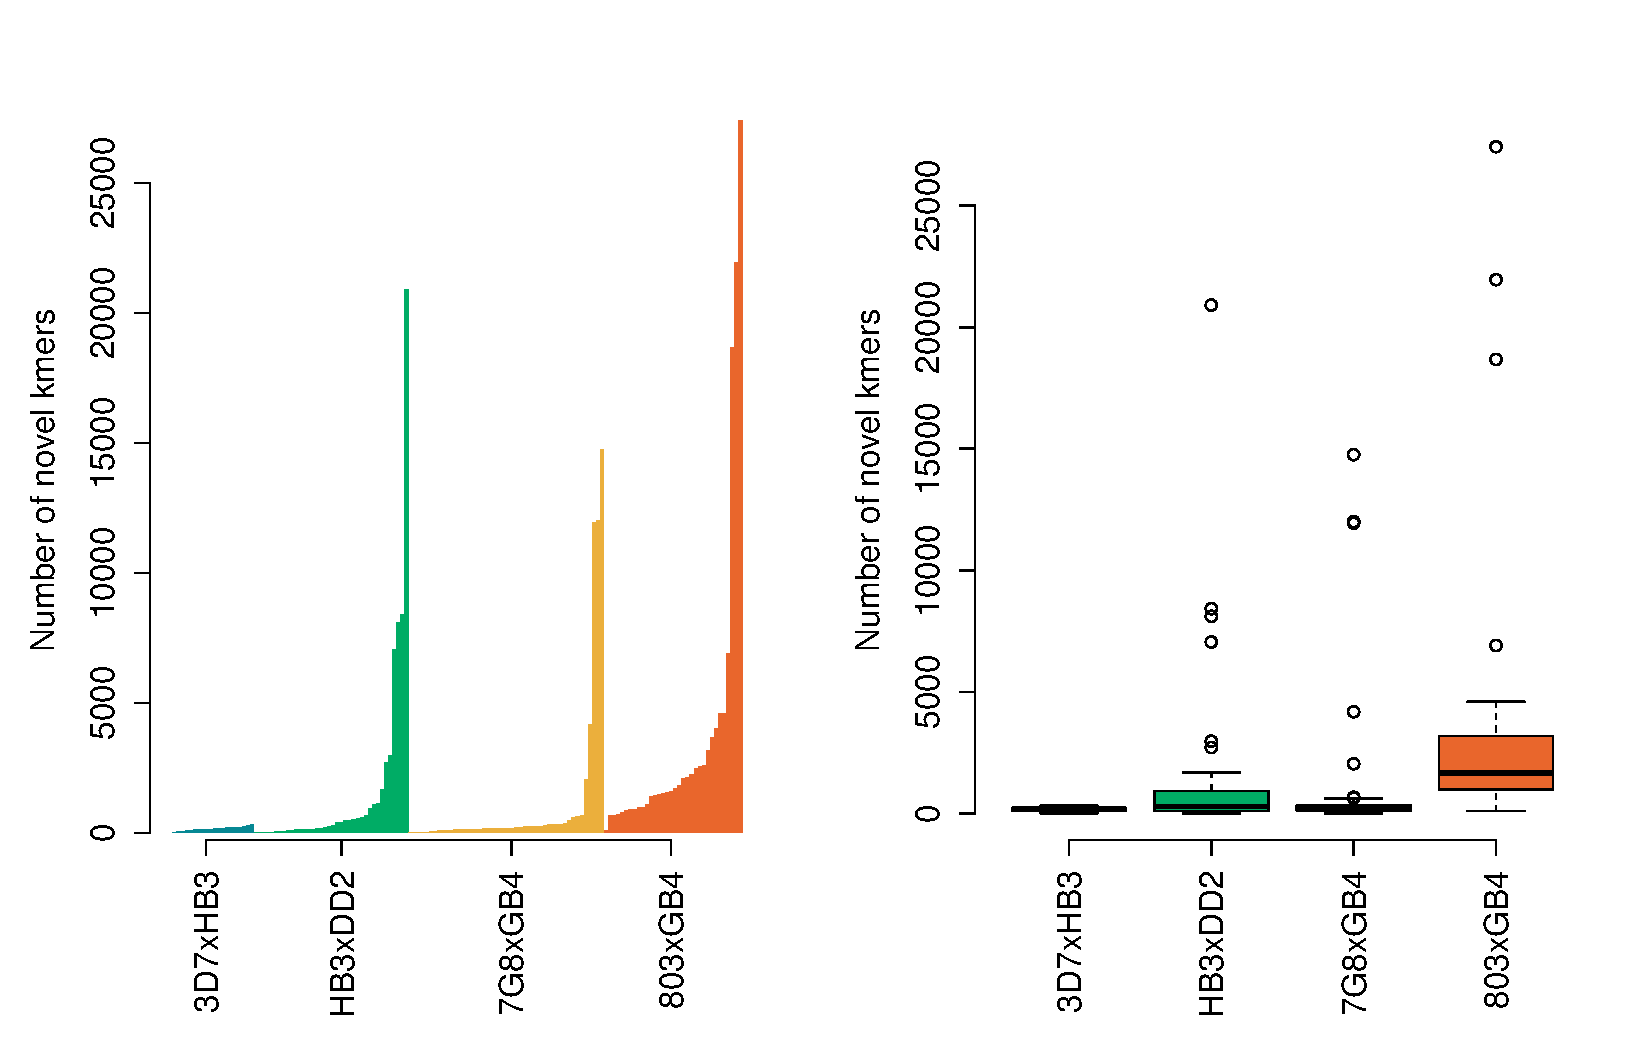
\includegraphics[width=\textwidth]{allnovelkmers-1}
  \caption{Novel kmers per sample and cross.  Left: number of novel kmers in each sample, after filtering.  Right: distribution of novel kmers per sample in each cross.}
  \label{fig:allnovelkmers-1}
\end{figure}

\begin{figure}[h!]
  \centering
    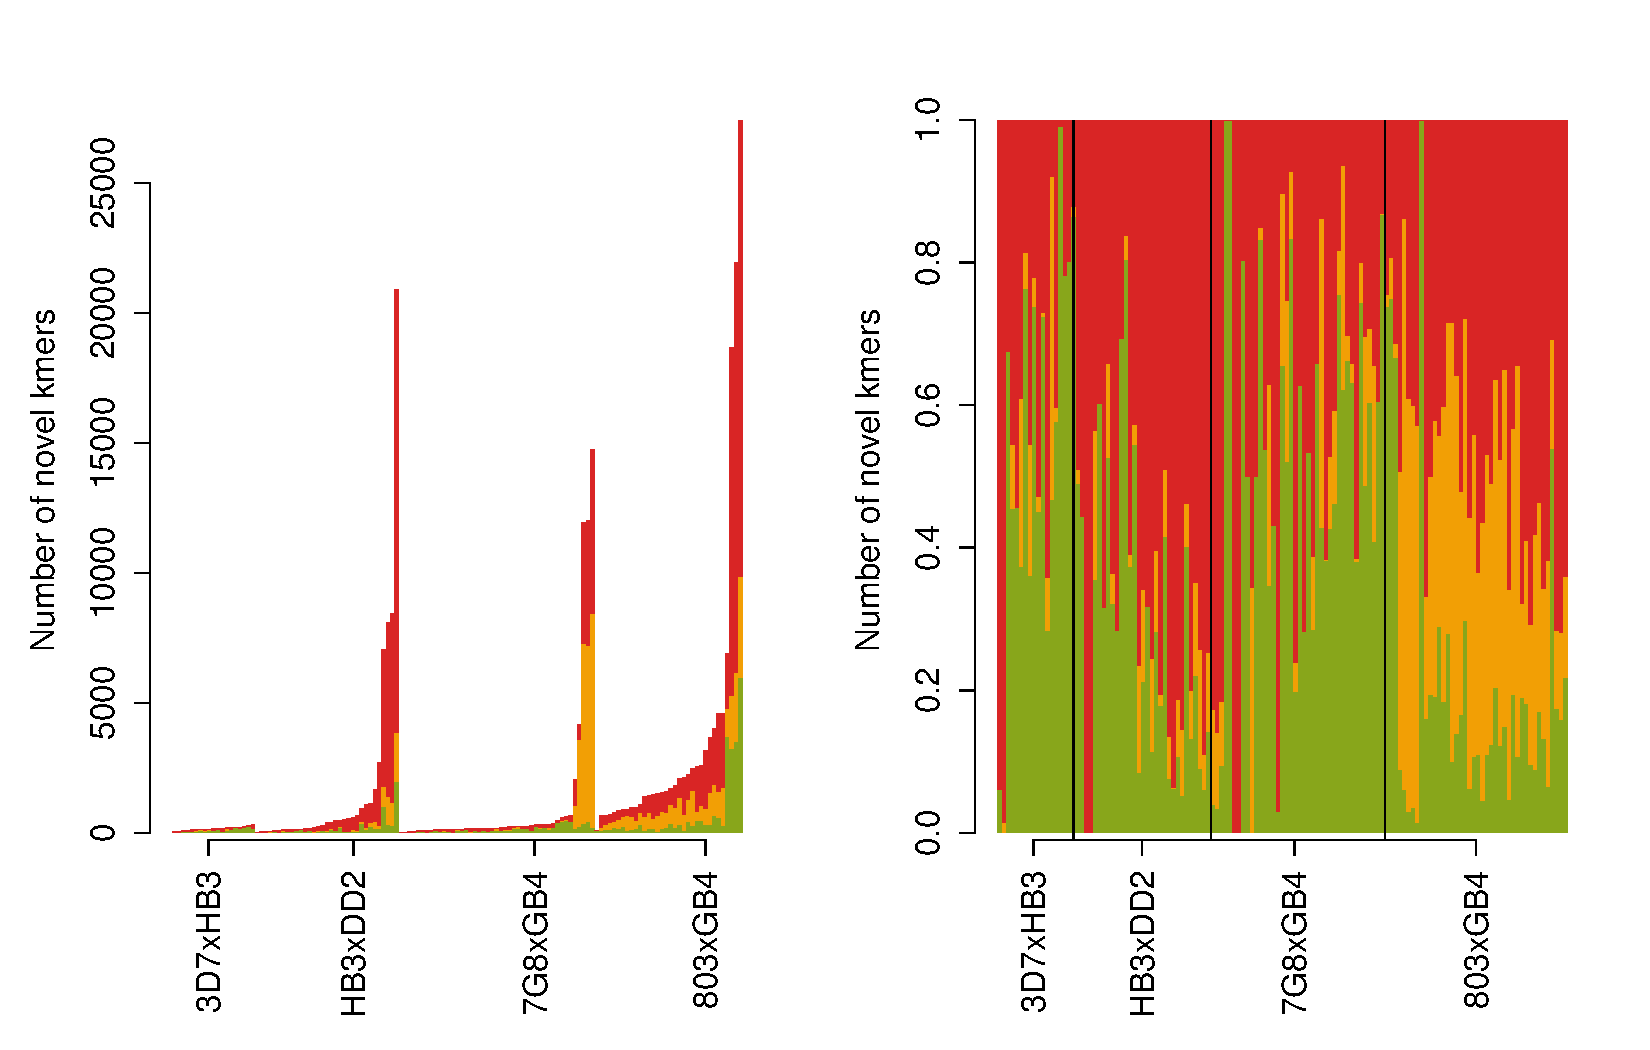
\includegraphics[width=\textwidth]{novelKmerUsage-1}
  \caption{Novel kmer usage by variants per sample and cross.  Left: novel kmers used in variants (green), in unknown events (orange), and events failing filters (red).  Right: fraction of novel kmers used by vaiants (green), unknown events (orange), and events failing filters (red).}
  \label{fig:novelKmerUsage-1}
\end{figure}

We applied our software to determine the number of novel kmers in all samples and all crosses.  These per-sample counts are shown in Figure \ref{fig:allnovelkmers-1}.  Counts are largely consistent across samples and crosses, typically ranging from a few hundred to a few thousand novel kmers.  Notably, the 803xGB4 samples have substantially more novel kmers than the other crosses.  While the median number of novel kmers per sample in the 3D7xHB3, HB3xDD2, and 7G8xGB4 crosses are $340$, $278$, and $173$ respectively, the median count in the 803xGB4 cross is $1,650$ with a very large variance.  Given that we've seen the larger-than-expected assembly lengths and a tremendous amount of data contamination, it seems likely that this excess is due to incomplete mitigation of those factors via our filtration process.  Rather than the samples harboring a vast amount of \textit{de novo} mutation activity, we expect to find a large fraction of calls in these samples to be unclassifiable.

Next, we applied our DNM calling software to all samples.  To see how many of the novel kmers were explained by variants passing filters, unknown events passing filters, or events failing filters, we superimposed the variant calls' novel kmer usage atop the total number of novel kmers per sample.  As evident in Figure \ref{fig:novelKmerUsage-1}, there is substantial variation between samples.  As predicted, many of the 803xGB4 variants are unclassified.  The median fraction of kmers explained by definable variants passing filters is a mere $29\%$, but when events failing filters are removed from consideration, this number jumps to $70\%$ of novel kmers explained.

\subsection{Variants per sample and cross}

Within each sample, we removed allelic variants appearing within the same gene as an NAHR event since, as we saw in the previous section, partial recovery of NAHR events can lead to erroneous accounting of the true mutation rates.  This rejects $211$ additional events, leaving us with $7,193$ that pass filters.

The monomorphic and polymorphic variants per sample and cross are summarized in Tables \ref{tbl:variantTableMono} and \ref{tbl:variantTablePoly}.  Behavior is largely consistent between samples and crosses.  Typically, each sample harbors only one or two monomorphic variants (presumably accumulated prior to or during meiosis), and fewer polymorphic variants (presumably accumulated during mitosis).  SNPs are the most common variant, followed by deletion events.  Insertions and multinucleotide polymorphisms occur rarely.  We detect no inversions.

At first glance, the 803xGB4 cross seems to harbor an unusual amount of NAHR activity.  However, we believe skepticism is warranted for this type of variant in this cross.  The key to detecting NAHR events is determining that many kmers co-localize on the same contig in the child but originate from different chromosomes in the parent.  With a poor 803 parental assembly constructed from short Illumina reads, many events may span multiple parental contigs but be part of the same chromosome.  A possible solution would be to align these parental contigs to the 3D7 reference and apply heuristics, rejecting any event where different contigs involved in the event align to the same chromosome.  However, this solution is not necessarily workable.  The assembled contigs are short, and the divergence between 803 and 3D7 is very high, particularly in the subtelomeric regions where true events almost certainly originate.  Therefore, alignment of the parental contigs to the 3D7 reference is not expected to solve the problem.  We have initiated an effort to have the 803 parent sequenced on PacBio instruments.  At of this writing, such data is not expected to be available for several months.

%\begin{figure}[h!]
%  \centering
%    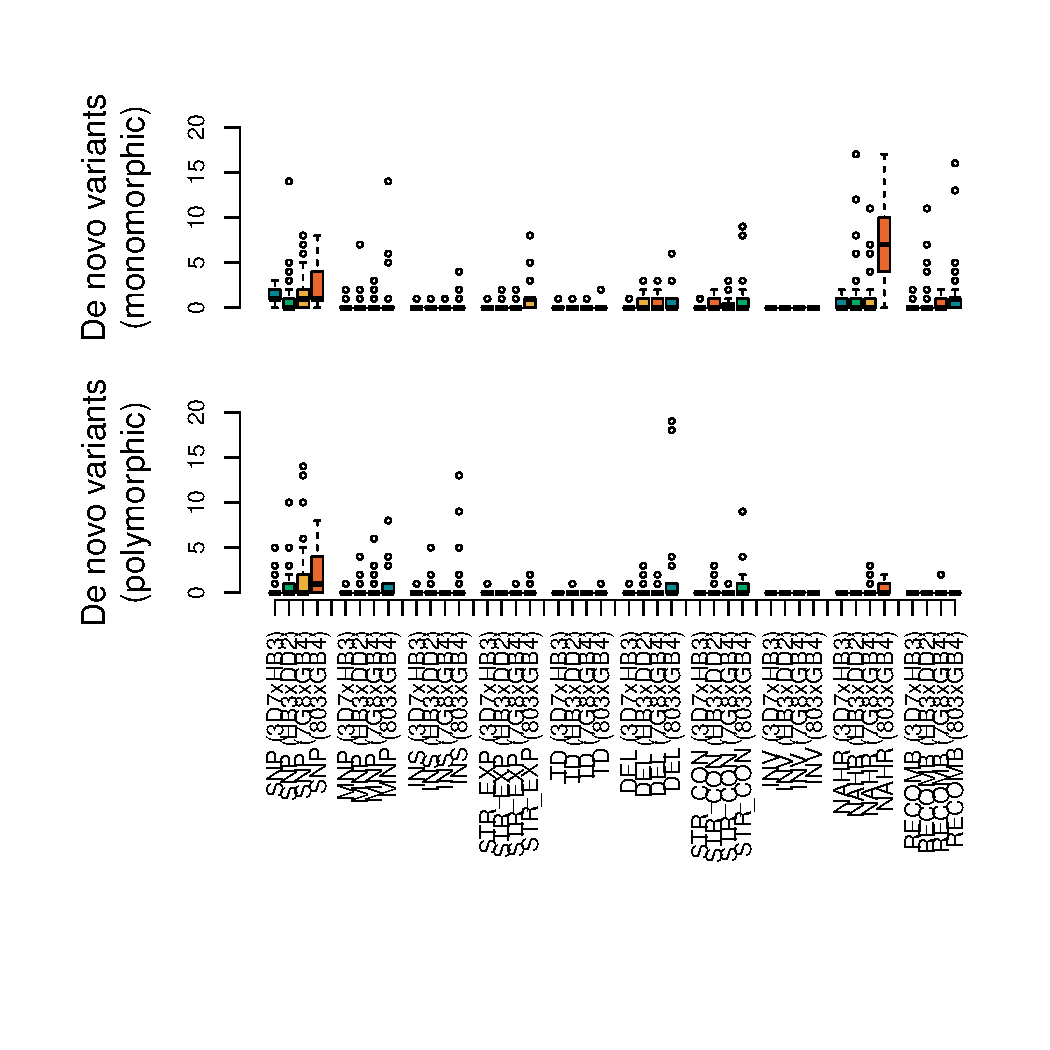
\includegraphics[width=\textwidth]{variantbarplot-1}
%  \caption{Variants per sample and cross.  Top: monomorphic variants.  Bottom: polymorphic variants.}
%  \label{fig:variantbarplot-1}
%\end{figure}

% Outstanding items
% 1. FDR
% 2. Verification (or refutation) of every known NAHR event
% 3. Rates

\begin{table}[]
\small
\centering
\caption{Monomorphic variants and rates of occurrence per cross and per sample}
\label{tbl:variantTableMono}
\begin{tabular}{rrrrr}
\toprule
                                   & 3D7xHB3                & HB3xDD2                & 7G8xGB4                & 803xGB4                   \\
\midrule
    \multicolumn{1}{l}{Samples}    & 20                     & 36                     & 26                     & 33                        \\
\addlinespace
    \multicolumn{1}{l}{SNP}        & $26$ $(1.37 \pm 1.07)$ & $45$ $(0.97 \pm 1.43)$ & $77$ $(1.05 \pm 1.38)$ & $187$ $(1.34 \pm 1.42)$   \\
\addlinespace
    \multicolumn{1}{l}{Insertions} & $3$ $(0.00 \pm 0.00)$  & $15$ $(0.38 \pm 0.61)$ & $13$ $(0.00 \pm 0.00)$ & $33$ $(0.52 \pm 0.69)$    \\
            \textit{STR expansion} & $1$ $(0.00 \pm 0.00)$  & $8$ $(0.00 \pm 0.00)$  & $8$ $(0.00 \pm 0.00)$  & $25$ $(0.45 \pm 0.51)$    \\
       \textit{Tandem duplication} & $1$ $(0.00 \pm 0.00)$  & $2$ $(0.00 \pm 0.00)$  & $3$ $(0.00 \pm 0.00)$  & $1$ $(0.00 \pm 0.00)$     \\
                    \textit{Other} & $1$ $(0.00 \pm 0.00)$  & $5$ $(0.00 \pm 0.00)$  & $2$ $(0.00 \pm 0.00)$  & $7$ $(0.00 \pm 0.00)$     \\
\addlinespace
     \multicolumn{1}{l}{Deletions} & $5$ $(0.26 \pm 0.45)$  & $35$ $(1.06 \pm 1.14)$ & $39$ $(0.66 \pm 0.73)$ & $41$ $(0.63 \pm 0.67)$    \\
          \textit{STR contraction} & $4$ $(0.00 \pm 0.00)$  & $13$ $(0.39 \pm 0.61)$ & $18$ $(0.28 \pm 0.55)$ & $17$ $(0.42 \pm 0.66)$    \\
                    \textit{Other} & $1$ $(0.00 \pm 0.00)$  & $22$ $(0.43 \pm 0.68)$ & $21$ $(0.41 \pm 0.58)$ & $24$ $(0.44 \pm 0.56)$    \\
\addlinespace
           \multicolumn{1}{l}{MNP} & $1$ $(0.00 \pm 0.00)$  & $17$ $(0.31 \pm 0.59)$ & $15$ $(0.00 \pm 0.00)$ & $50$ $(0.00 \pm 0.00)$    \\
                \textit{Inversion} & $0$ $(0.00 \pm 0.00)$  & $0$ $(0.00 \pm 0.00)$  & $0$ $(0.00 \pm 0.00)$  & $0$ $(0.00 \pm 0.00)$     \\
                    \textit{Other} & $1$ $(0.00 \pm 0.00)$  & $17$ $(0.31 \pm 0.59)$ & $15$ $(0.00 \pm 0.00)$ & $0$ $(0.00 \pm 0.00)$     \\
\addlinespace
          \multicolumn{1}{l}{NAHR} & $6$ $(0.00 \pm 0.00)$  & $13$ $(0.00 \pm 0.00)$ & $4$ $(0.00 \pm 0.00)$  & $15$ $(0.00 \pm 0.00)$    \\
 \multicolumn{1}{l}{Recombination} & $6$ $(0.00 \pm 0.00)$  & $32$ $(0.00 \pm 0.00)$ & $19$ $(0.42 \pm 0.58)$ & $59$ $(0.54 \pm 0.58)$    \\
\addlinespace
       \multicolumn{1}{l}{unknown} & $21$ $(0.00 \pm 0.00)$ & $828$ $(0.00 \pm 0.00)$ & $1548$ $(0.00 \pm 0.00)$   & $1513$ $(0.00 \pm 0.00)$    \\
\bottomrule
\end{tabular}
\end{table}

\begin{table}[]
\small
\centering
\caption{Polymorphic variants and rates of occurrence per cross and per sample}
\label{tbl:variantTablePoly}
\begin{tabular}{rrrrr}
\toprule
                                   & 3D7xHB3                & HB3xDD2                & 7G8xGB4                 & 803xGB4                   \\
\midrule
    \multicolumn{1}{l}{Samples}    & 20                     & 36                     & 26                      & 33                        \\
\addlinespace
    \multicolumn{1}{l}{SNP}        & $11$ $(0.00 \pm 0.00)$ & $96$ $(0.38 \pm 0.73)$ & $149$ $(0.62 \pm 1.14)$ & $207$ $(1.66 \pm 2.02)$   \\
\addlinespace
    \multicolumn{1}{l}{Insertions} & $2$ $(0.00 \pm 0.00)$  & $16$ $(0.00 \pm 0.00)$ & $1$ $(0.00 \pm 0.00)$   & $35$ $(0.00 \pm 0.00)$    \\
            \textit{STR expansion} & $1$ $(0.00 \pm 0.00)$  & $0$ $(0.00 \pm 0.00)$  & $0$ $(0.00 \pm 0.00)$   & $30$ $(0.00 \pm 0.00)$    \\
       \textit{Tandem duplication} & $0$ $(0.00 \pm 0.00)$  & $2$ $(0.00 \pm 0.00)$  & $1$ $(0.00 \pm 0.00)$   & $4$ $(0.00 \pm 0.00)$     \\
                    \textit{Other} & $1$ $(0.00 \pm 0.00)$  & $14$ $(0.00 \pm 0.00)$ & $0$ $(0.00 \pm 0.00)$   & $1$ $(0.00 \pm 0.00)$     \\
\addlinespace
     \multicolumn{1}{l}{Deletions} & $1$ $(0.00 \pm 0.00)$  & $17$ $(0.00 \pm 0.00)$ & $10$ $(0.00 \pm 0.00)$  & $214$ $(0.00 \pm 0.00)$    \\
          \textit{STR contraction} & $0$ $(0.00 \pm 0.00)$  & $7$ $(0.00 \pm 0.00)$  & $8$ $(0.00 \pm 0.00)$   & $71$ $(0.17 \pm 0.38)$    \\
                    \textit{Other} & $1$ $(0.00 \pm 0.00)$  & $10$ $(0.00 \pm 0.00)$ & $2$ $(0.00 \pm 0.00)$   & $143$ $(0.28 \pm 0.59)$    \\
\addlinespace
           \multicolumn{1}{l}{MNP} & $1$ $(0.00 \pm 0.00)$  & $11$ $(0.00 \pm 0.00)$ & $34$ $(0.00 \pm 0.00)$  & $31$ $(0.00 \pm 0.00)$    \\
                \textit{Inversion} & $0$ $(0.00 \pm 0.00)$  & $0$ $(0.00 \pm 0.00)$  & $0$ $(0.00 \pm 0.00)$   & $0$ $(0.00 \pm 0.00)$     \\
                    \textit{Other} & $1$ $(0.00 \pm 0.00)$  & $0$ $(0.00 \pm 0.00)$  & $34$ $(0.00 \pm 0.00)$  & $31$ $(0.00 \pm 0.00)$     \\
\addlinespace
          \multicolumn{1}{l}{NAHR} & $0$ $(0.00 \pm 0.00)$  & $0$ $(0.00 \pm 0.00)$  & $0$ $(0.00 \pm 0.00)$   & $0$ $(0.00 \pm 0.00)$    \\
 \multicolumn{1}{l}{Recombination} & $0$ $(0.00 \pm 0.00)$  & $0$ $(0.00 \pm 0.00)$  & $2$ $(0.00 \pm 0.00)$   & $0$ $(0.00 \pm 0.00)$    \\
\bottomrule
\end{tabular}
\end{table}

\subsection{Manual examination of every event in the 3D7xHB3 cross}

To estimate a false discovery rate, we manually examined all $83$ monomorphic and polymorphic events in the 3D7xHB3 cross using our graph visualization software and IGV.  $50/83$ events appear to have clear support in both visualizations.  The vast majority of these events are so-called bubble-motif variants, with the exception of the NAHR event in PG0063-C and an unknown event (a misclassification - an event is called in the correct location, but upon closer inspection, appears to be two biallelic SNPs in close proximity, confusing the calling software).  Another $12$ events had uncertain validation status; one was a putative NAHR event, another was a recombination event, two were polymorphic variants, and the remaining $8$ could not be typed.  Finally, $25$ events were clear false-positives owing to various issues (e.g. proximity to a repetitive region or otherwise appearing artifactual).  The bulk of such events could not be typed ($12$) or were non-bubble-motif ($7$).  It was rare for bubble-motif variants to manifest as false-positives; occuring for a single insertion and $5$ SNPs.  In the case of the SNPs, all false-positives appeared as a result of misclassifying an inherited event as \textit{de novo} due to the mutations' proximity to another event - usually a polymorphic variant.  The polymorphic event makes it appear that the haplotypic background of the variant is different from the true background which contains the SNP.  Thus, when our caller goes to examine the evidence, it finds novel kmers due to the polymorphic event, finds the inherited mutation in close proximity, misassociates the two, and calls the variant.

Ignoring untyped events and pessimistically assuming that any event with uncertain validation status was false, we estimate our FDR to be $18/68$, or approximately $26\%$.  However, we should expect that NAHR and recombination events carry a much higher false-positive rate and drive the bulk of this estimate.  After removing these events from consideration, we find our FDR is $9/54$, or approximately $16\%$.

\subsection{Recovery of published \textit{var} gene recombinations}

The underlying dataset for our study was partially available to Claessens \textit{et al.} at the time of their study.  In their reference-based work, Claessens \textit{et al.} identified many \textit{var} gene recombinations involving exon $1$, including subtelomeric members and centrally-located members of the gene family.  As core \textit{var} gene recombinations have not been reported in the past, we sought to confirm these events with our reference-free methods.  The calls from Claessens \textit{et al.} and our study are summarized in Table \ref{tbl:nahrcompare}.  Of the $12$ calls they make in the shared 3D7xHB3 and HB3xDD2 samples, a single event is recapitulated by our graphical method: the well-known PG0063-C event.  $6$ more of their events find no visual support in our reference-free kmer accounting method, which would otherwise indicate some sort of structural variant activity (even it is unable to prove that the event occured between two specific genes in question).  $3$ more events do show some signs of NAHR activity, but not between the genes listed by Claessens \textit{et al.}.  No recombinations between core \textit{var} genes validate visually.

In contrast, examining the 3D7xHB3 and HB3xDD2 crosses, we find $5$ events, all of which are supported by the kmer recovery diagnostic plots.  Figure \ref{fig:kmerrecoverytpfp} shows an example of a seemingly false-positive core \textit{var} gene recombination (a) and a true event (b).

\begin{table}[]
\centering
\caption{NAHR events in Claessens \textit{et al.} and this study}
\label{tbl:nahrcompare}
\begin{tabular}{@{}lllll@{}}
\toprule
Sample    & Cross   & Called in Claessens \textit{et al.} & Called in this study & Support in kmer recovery \\ \midrule
PG0015-C  & HB3xDD2 & n                         & y                    & y                        \\
PG0018-C  & HB3xDD2 & n                         & y                    & y                        \\
PG0020-C  & HB3xDD2 & y                         & n                    & n                        \\
PG0025-C  & HB3xDD2 & n                         & y                    & n                        \\
PG0030-C  & HB3xDD2 & y                         & n                    & n                        \\
PG0034-C  & HB3xDD2 & y                         & n                    & y                        \\
PG0035-Cx & HB3xDD2 & n                         & y                    & n                        \\
PG0036-C  & HB3xDD2 & y                         & n                    & wrong genes              \\
PG0038-C  & HB3xDD2 & y                         & n                    & y                        \\
PG0044-C  & HB3xDD2 & y                         & n                    & n                        \\
PG0054-C  & 3D7xHB3 & y                         & n                    & n                        \\
PG0055-C  & 3D7xHB3 & n                         & y                    & y                        \\
PG0058-C  & 3D7xHB3 & y                         & n                    & wrong gene               \\
PG0063-C  & 3D7xHB3 & y                         & y                    & y                        \\
PG0067-C  & 3D7xHB3 & n                         & y                    & n                        \\
PG0068-C  & 3D7xHB3 & y                         & n                    & n                        \\
PG0069-C  & 3D7xHB3 & y                         & n                    & n                        \\
PG0070-C  & 3D7xHB3 & n                         & y                    & n                        \\
PG0071-C  & 3D7xHB3 & n                         & y                    & y                        \\
PG0072-C  & 3D7xHB3 & y                         & n                    & wrong gene               \\
PG0079-CW & 7G8xGB4 & y                         & n                    & NA                       \\
PG0082-C  & 7G8xGB4 & y                         & n                    & NA                       \\
PG0085-C  & 7G8xGB4 & y                         & y                    & NA                       \\
PG0087-C  & 7G8xGB4 & y                         & n                    & NA                       \\
PG0088-C  & 7G8xGB4 & y                         & y                    & NA                       \\
PG0095-C  & 7G8xGB4 & y                         & n                    & NA                       \\
PG0100-CW & 7G8xGB4 & y                         & n                    & NA                       \\
PG0103-CW & 7G8xGB4 & y                         & n                    & NA                       \\
PG0105-CW & 7G8xGB4 & y                         & n                    & NA                       \\
PG0107-C  & 7G8xGB4 & y                         & n                    & NA                       \\
PG0112-C  & 7G8xGB4 & NA                        & y                    & NA                       \\
PG0113-C  & 7G8xGB4 & NA                        & y                    & NA                       \\
PG0444-C  & 803xGB4 & NA                        & y                    & NA                       \\
PG0456-C  & 803xGB4 & NA                        & y                    & NA                       \\
PG0459-C  & 803xGB4 & NA                        & y                    & NA                       \\
PG0468-C  & 803xGB4 & NA                        & y                    & NA                       \\
PG0469-C  & 803xGB4 & NA                        & y                    & NA                       \\ \bottomrule
\end{tabular}
\end{table}

\begin{figure}[h!]
  \centering
    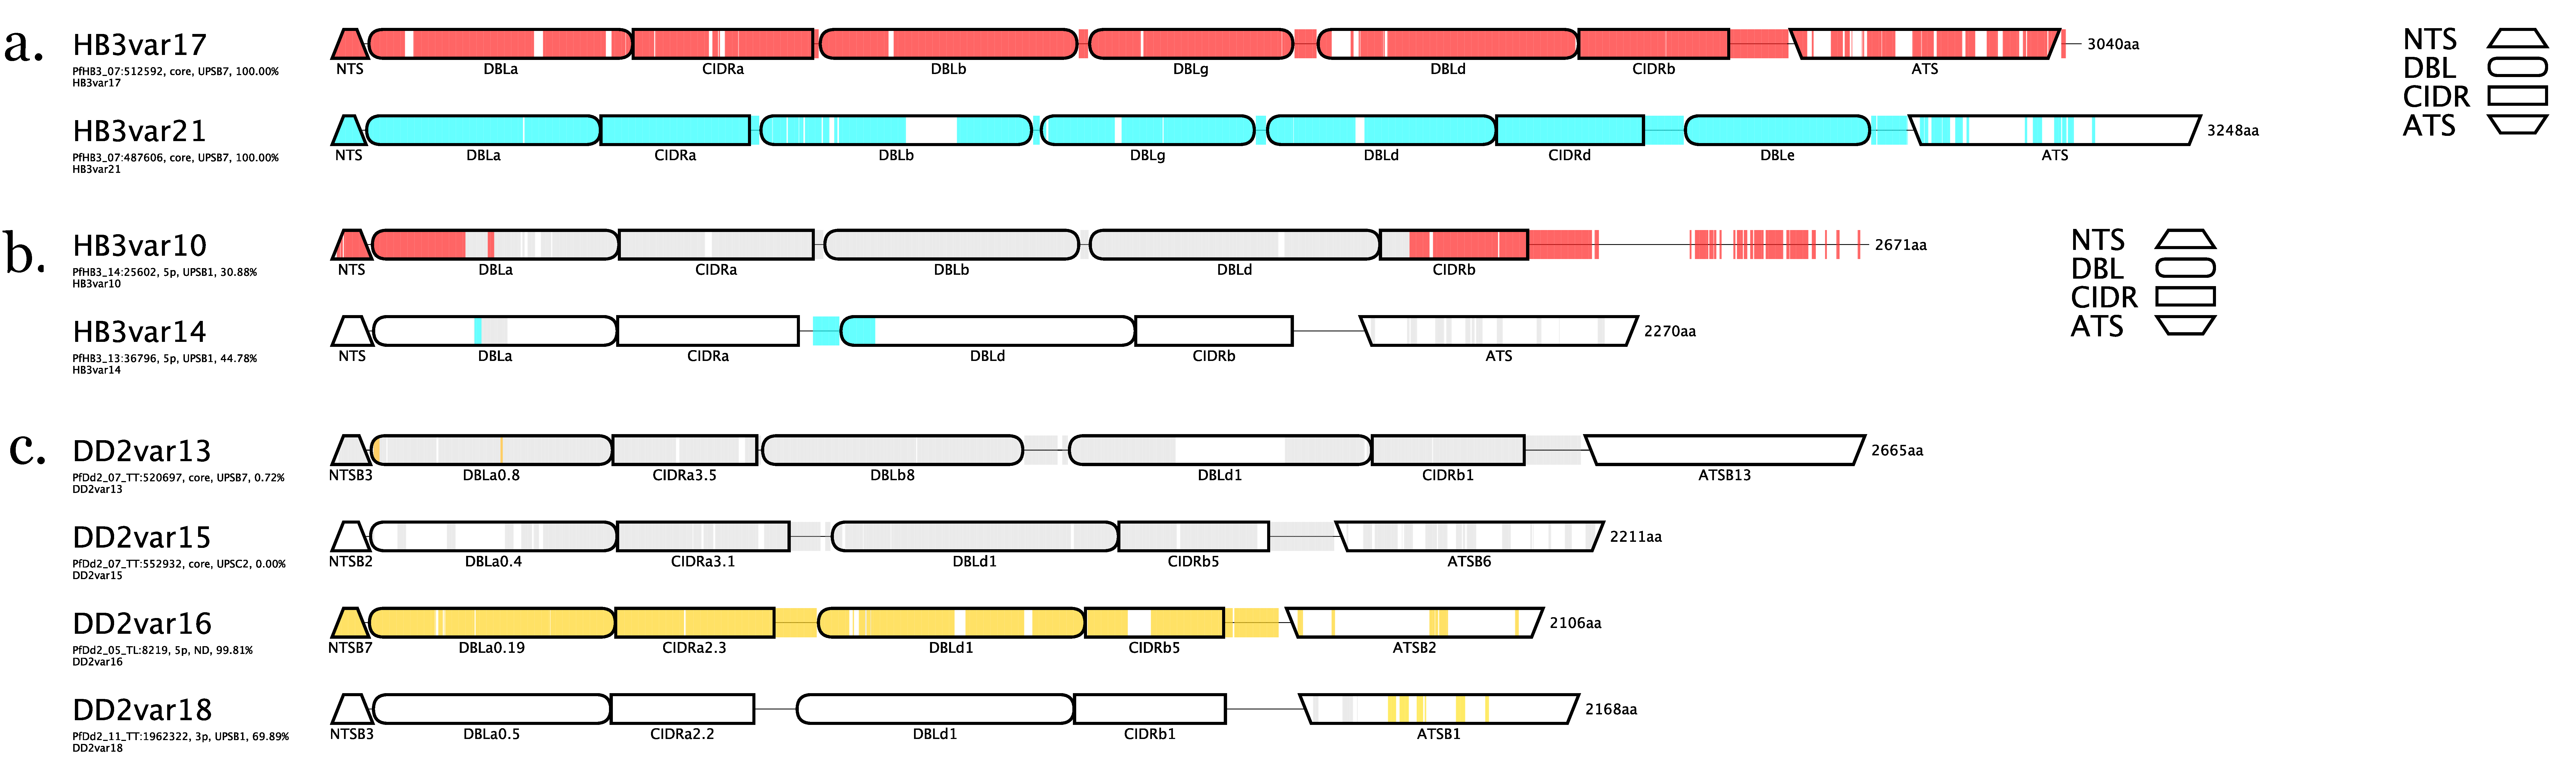
\includegraphics[width=\textwidth]{kmerrecoverytpfp}
  \caption{Recovery of diagnostic kmers in 3D7 and HB3 \textit{var} genes.  White regions indicate kmers that were not diagnostic.  Vertical grey indicates a diagnostic kmer that absent in the progeny, while vertical colored lines indicate the kmer's presence.  a. Two genes in PG0020-C purported to have an NAHR event in Claessens \textit{et al.}, but exhibiting no kmer loss indicative of an NAHR event.  b. Two genes in PG0034-C with missing diagnostic kmers, possibly indicative of an NAHR event.  c. Two genes (DD2var13 and DD2var18) which exhibit very slight recovery or loss of diagnostic kmers towards their terminal ends.}
  \label{fig:kmerrecoverytpfp}
\end{figure}
